%%%%%%%%%%%%%%%%%%%%%%%%%%%%%%%%%%%%%%%%%%%%%%%%%%%%%%%%%%%%%%%%%%%%%%%%%%%%%%
% ASU Dissertation Template
%%%%%%%%%%%%%%%%%%%%%%%%%%%%%%%%%%%%%%%%%%%%%%%%%%%%%%%%%%%%%%%%%%%%%%%%%%%%%%
% Copyright 2019 Robert W. Kutter (robert@kutterconsulting.com)
%
%   See also: http://kutterconsulting.com
%
% For guidance on using this file, see the README.
%
%%%%%%%%%%%%%%%%%%%%%%%%%%%%%%%%%%%%%%%%%%%%%%%%%%%%%%%%%%%%%%%%%%%%%%%%%%%%%%
% Preamble
%%%%%%%%%%%%%%%%%%%%%%%%%%%%%%%%%%%%%%%%%%%%%%%%%%%%%%%%%%%%%%%%%%%%%%%%%%%%%%
\newcommand*{\pointsize}{12pt}          %<Set the font size; make sure the size is correct
                                        %   for the font you will use
\documentclass[letterpaper,             % Use US letter-size paper
               oneside,                 % No verso and recto differences
               \pointsize]              % Uses the font size defined above
               {memoir}
\renewcommand{\cleardoublepage}%        % \cleardoublepage will create entirely blank
  {\clearpage}%                         %   pages depending on settings (e.g., usually
                                        %   before start of \mainmatter); redefine it here
                                        %   so that no entirely blank pages are created
                                        %   automatically
%%%%%%%%%%%%%%%%%%%%%%%%%%%%%%%%%%%%%%%
% (Some) Packages
%%%%%%%%%%%%%%%%%%%%%%%%%%%%%%%%%%%%%%%
\usepackage{graphicx}                   % For importing image files
\usepackage{etoolbox}                   % For advanced commands throughout preamble
\usepackage{microtype}                  %~Improves kerning and protrusion (optional);
                                        %   See here for an introduction:
                                        %   http://www.khirevich.com/latex/microtype/
\usepackage{bm}                         % for both math
\providetoggle{usemicrotype}            % TRUE = microtype is being used
\makeatletter                           %   (Used to turn of microtype protrusion in the
\@ifpackageloaded{microtype}%           %   table of contents.)
  {\settoggle{usemicrotype}{true}}%
  {\settoggle{usemicrotype}{false}}
\makeatother
\usepackage{changepage}                 % For changing page layout (e.g., margins) in the
                                        %   middle of the document
\usepackage{calc}					              % Calculate text widths; used in page layout
                                        %   changes
% \usepackage{caption}
\usepackage{subfigure}
\usepackage{tabstackengine}

%%%%%%%%%%%%%%%%%%%%%%%%%%%%%%%%%%%%%%%
% Title page, input
%%%%%%%%%%%%%%%%%%%%%%%%%%%%%%%%%%%%%%%
\listadd{\titlelines}%
  {Design, Development, and Modeling of a Novel Underwater Vehicle for}             %<Enter the title of the dissertation
\listadd{\titlelines}%
  {Autonomous Reef Monitoring}            % If you want to
                                        %   split the title across lines,
                                        %   use another \listadd command for the
                                        %   second line
\newcommand*\Author{Alex Goldman}                      %<Enter your name; must match official transcript
\newcommand*{\documentname}%
  {Thesis}                        %<Enter the type of document (capitalized)
\newcommand*{\degreename}
  {Master of Science}                %<Enter the type of degree (capitalized)
\newcommand*\defdate{November 2020}                       %<Give month (written out fully) and year of
                                        %   the oral defense
\listadd{\committeechair}{Jnaneshwar Das}   %<Enter committee chair name; use \listadd for
%\listadd{\committeechair}{Another name}%   for additional names
\newcommand*{\chairlabel}{Chair}        %<If you have co-chairs, replace this text with
                                        %   'Co-Chair'
\listadd{\committeemember}{Greg Asner} %<Enter committee member names; use \listadd for
\listadd{\committeemember}{Hamidreza Marvi} %   additional names
\newcommand*{\gradmonth}{December}         %<Enter the graduation date; month can only be:
                                        %  May, August, or December
\newcommand*{\gradyear}{2020}           %<Enter the graduation year, e.g. 2014

\listadd{\keywords}{keyword 1}          %<Enter keywords; use \listadd for
\listadd{\keywords}{keyword 2}          %   additional names (up to 6)
\newcommand*{\graddate}{\gradmonth%     % Compose full graduation date
  \space\gradyear}

%%%%%%%%%%%%%%%%%%%%%%%%%%%%%%%%%%%%%%%
% Page layout
%%%%%%%%%%%%%%%%%%%%%%%%%%%%%%%%%%%%%%%
\settrimmedsize{\stockheight}%          % Specifies \paperheight and \paperwidth
  {\stockwidth}{*}
\settrims{0pt}{0pt}                     % Set location of page in relation to the stock.
                                        % Paper and stock size are equivalent,
                                        % so both \trimtop and \trimedge are set to 0pt
\newlength{\forfootskip}
\setlength{\forfootskip}%
  {3\baselineskip}
\newlength{\textblockheight}            % Calculate height of text block to leave room
\setlength{\textblockheight}{9.0in}     %   for footers, keeping page numbers outside
\addtolength{\textblockheight}%         %   the 1in vertical margins
  {-\forfootskip}
\settypeblocksize{\textblockheight}%    % Calculated by 1.0in vertical margins and
  {*}{*}                                %   letting margins set the width of the typeblock
\setulmargins{1.0in}{*}{*}              % Set upper margin (\uppermargin, not \topmargin);
                                        %   calculate the bottom margin
\setlrmarginsandblock{1.25in}{1.25in}{*}%~Set margins and calculate width of typeblock
\setheaderspaces{*}{0.5\baselineskip}{*}% Arguments: '\headdrop', '\headsep', and/or ratio
                                        %   Note: This is only used in the list of
                                        %   contents sections
\setheadfoot{\baselineskip}%            % Set '\headheight' and '\footskip'
  {\forfootskip}
\checkandfixthelayout                   % Required by memoir package after setting layout
\settypeoutlayoutunit{in}               % Write layout dimensions to log file in inches

%%%%%%%%%%%%%%%%%%%%%%%%%%%%%%%%%%%%%%%
% Fonts
%%%%%%%%%%%%%%%%%%%%%%%%%%%%%%%%%%%%%%%
\usepackage[T1]{fontenc}                % Standard option to handle, e.g., accented
                                        %   characters like 'ö' better
\usepackage{amssymb,mathtools}          % For AMS-LaTeX, see here for more:
                                        %     http://www.ams.org/publications/authors/tex/amslatex
                                        % ('mathtools' loads and extends 'amsmath')
\usepackage{ifxetex,ifluatex}           % Can check if XeTeX or LuaTeX was used to typeset
\usepackage{fixltx2e}                   % Provides \textsubscript
\IfFileExists{upquote.sty}%             % Use upquote if available, for
  {\usepackage{upquote}}{}              %   straight quotes in verbatim environments

% Load fonts depending on the
%   typesetting engine
\ifnum 0\ifxetex 1\fi\ifluatex 1\fi=0   % If pdftex
  \usepackage[utf8]{inputenc}           %   'utf8' should match the encoding of this file
                                        %
                                        %~Set up your font in pdftex here
                                        %
\else 									                % If xetex or luatex
  \ifxetex                              % If xetex
    \usepackage{mathspec}               % Matches non-math open-type font to math
                                        %   open-type font (use 'mathspec' if you want to
                                        %   write math in unicode)
    \usepackage{xunicode}               % Convert LaTeX character macros to unicode
  \else                                 % If luatex\usepackage{fontspec}
    \usepackage{fontspec}               % Use fontspec for (open type) font selection
  \fi
  \defaultfontfeatures{Mapping=tex-text,% Font spec setting
    Scale=MatchLowercase}
  \newcommand*{\euro}{€}
  \setmainfont{Garamond}                %<Set the main font; make sure the font is correct
                                        %   for the font size (See ASU Style Guide)
%  \setmathfont(Digits,Latin,Greek)%     %~Uncomment two lines to set a font for math%
%    {MATHFONT}
\fi

%%%%%%%%%%%%%%%%%%%%%%%%%%%%%%%%%%%%%%%
% Line spacing
%%%%%%%%%%%%%%%%%%%%%%%%%%%%%%%%%%%%%%%
\DoubleSpacing                          % True double spacing
\BeforeBeginEnvironment{quote}          % Memoir leaves most special material
  {\par\SingleSpacing}                  %   single spaced, but makes block quotes
\AfterEndEnvironment{quote}%            %   double-spaced; fix to follow ASU style guide
  {\vspace{-\baselineskip} %
  \DoubleSpacing}
\BeforeBeginEnvironment{quotation}%
  {\par\SingleSpacing}
\AfterEndEnvironment{quotation}%
  {\vspace{-\baselineskip} %
  \DoubleSpacing}

\setlength{\footnotesep}{\baselineskip} % Double space *between* footnotes
\renewcommand*{\footnoterule}{%         % Redefine footnoterule so that initial footnote
  \kern-3pt%                            %   still appears right under the rule (changing
  \hrule width 0.4\columnwidth          %   \footnotesep also changes the space between the
  \kern 2.6pt                           %   rule and the first footnote
  \vspace{-0.5\baselineskip}            % (Here is the vertical space adjustment)
  }

\usepackage{enumitem}                   % Control spacing in enumerate environment
\setlist{noitemsep}                     % Remove extra vertical spacing between items in lists
                                        % \setlist{nosep} to leave no space around whole list

%%%%%%%%%%%%%%%%%%%%%%%%%%%%%%%%%%%%%%%
% Page numbering
%%%%%%%%%%%%%%%%%%%%%%%%%%%%%%%%%%%%%%%
\makepagestyle{ASU}
  \makeevenfoot{ASU}{}{\thepage}{}
  \makeoddfoot{ASU}{}{\thepage}{}

%%%%%%%%%%%%%%%%%%%%%%%%%%%%%%%%%%%%%%%
% Title page, formatting
%%%%%%%%%%%%%%%%%%%%%%%%%%%%%%%%%%%%%%%
\newlength{\savedfootskip}
\setlength{\savedfootskip}{\footskip}
\newcommand{\titlepagesetup}{%          % Page layout for title page
  \changepage%                          % Adjustment to page dimensions:
    {\savedfootskip}%                   %   text height
    {}%                                 %   text width
    {}%                                 %   even-side margin
    {}%                                 %   odd-side margin
    {}%                                 %   column sep.
    {}%                                 %   topmargin
    {}%                                 %   headheight
    {}%                                 %   headsep
    {-\savedfootskip}%                  %   footskip
}

\newcommand{\closetitlepagesetup}{%     % Undo set up for title page
  \changepage{-\savedfootskip}{}{}{}{}%
    {}{}{}{\savedfootskip}%
}

\makeatletter                           % Do not modify this section; Enter info above
\newcommand*{\titlepageASU}{
  \titlepagesetup
  \clearpage
  \begin{center}
  \SingleSpacing
  \thispagestyle{empty}
    \renewcommand*{\do}[1]{##1 \\[\baselineskip]}
    \dolistloop{\titlelines}
    by \\[\baselineskip]
    \Author \\[4\baselineskip]
    A \documentname~Presented in Partial Fulfillment \\
    of the Requirements for the Degree \\
    \degreename \\
    \vfill                              % Vertically center the portion below
    Approved \defdate~by the \\
    Graduate Supervisory Committee: \\[\baselineskip]
    \renewcommand*{\do}[1]{##1, \chairlabel \\}
    \dolistloop{\committeechair}
    \renewcommand*{\do}[1]{##1 \\}
    \dolistloop{\committeemember}
    \vfill                              % Vertically center the portion above
    ARIZONA STATE UNIVERSITY \\[\baselineskip]
    \graddate
  \end{center}
  \clearpage
  \closetitlepagesetup
}
\makeatother

%%%%%%%%%%%%%%%%%%%%%%%%%%%%%%%%%%%%%%%
% Heading styles
%%%%%%%%%%%%%%%%%%%%%%%%%%%%%%%%%%%%%%%
% Note: memoir also has \book and \part commands; do not use these
\makechapterstyle{ASU}{%                % Define chapter heading style
  \renewcommand*{\chapterheadstart}{}   % Chapter title flush with top margin
  \renewcommand*{\chapnamefont}%        % Set font for 'Chapter' or 'Appendix'
    {\normalfont}
  \renewcommand*{\chapnumfont}%         % Set font for number in chapter headings
    {\normalfont}
  \renewcommand*{\afterchapternum}%     % Insert a double line break after
    {\\[\baselineskip]}                 %   chapter number
  \renewcommand*{\chaptitlefont}%       % Set font for chapter title name
    {\normalfont}
  \setlength{\afterchapskip}{0pt}       % Set vertical space between chapter title and
                                        %   first paragraph; equivalent to one line break
                                        %   (vertical space = \afterchapskip + \baselineskip)
                                        % Note: This \afterchapskip value is only used in
                                        %   front matter
  \renewcommand*{\printchapternum}{%    % Center justify chapter number
    \centering \chapnumfont %
    \thechapter}
  \renewcommand*{\printchaptertitle}[1]%% Center justify
    {\expandafter\centering %           %   \MakeUppercase has issues; see here for some
    \expandafter\chaptitlefont %        %   details: https://tex.stackexchange.com/questions/35680/uppercase-in-newcommand
    \expandafter\MakeUppercase %        %   Accented characters and some fonts may not
    \expandafter{##1}}                  %   uppercase correctly; if that happens, just
                                        %   type the chapter title in uppercase
}

\setsecnumdepth{all}                    %~Enter the levels that you want to have numbered
                                        %   (Default is to number all [5 levels deep].)

\newcommand{\divisionbeforeskip}%       % Create default formatting for headings
  {\baselineskip}
\newcommand{\divisionindent}%
  {0.5em}
\newcommand{\divisionfont}{\normalfont} % Font must be \normalfont
\newcommand{\divisionafterskip}%
  {\baselineskip}

\setbeforesecskip{\divisionbeforeskip}  % Apply default formatting to all heading levels
\setsecindent{\divisionindent}          % Note: If you change \setsecnumdepth above, you
\setsecheadstyle{\divisionfont}         %   will need to set the indent for all lower
\setaftersecskip{\divisionafterskip}    %   levels to '0pt'; otherwise, they will be
                                        %   preceded by unnecessary space
\setbeforesubsecskip{\divisionbeforeskip}
\setsubsecindent{\divisionindent}
\setsubsecheadstyle{\divisionfont}
\setaftersubsecskip{\divisionafterskip}

\setbeforesubsubsecskip{\divisionbeforeskip}
\setsubsubsecindent{\divisionindent}
\setsubsubsecheadstyle{\divisionfont}
\setaftersubsubsecskip{\divisionafterskip}

\setbeforeparaskip{\divisionbeforeskip}
\setparaindent{\divisionindent}
\setparaheadstyle{\divisionfont}
\setafterparaskip{\divisionafterskip}

\setbeforesubparaskip{\divisionbeforeskip}
\setsubparaindent{\divisionindent}
\setsubparaheadstyle{\divisionfont}
\setaftersubparaskip{\divisionafterskip}

%%%%%%%%%%%%%%%%%%%%%%%%%%%%%%%%%%%%%%%
% Paragraph formatting
%%%%%%%%%%%%%%%%%%%%%%%%%%%%%%%%%%%%%%%
%\sloppybottom                          % Reduce the chances of widows
\raggedbottom                           % Loosens vertical spacing requirements, so
                                        %   \sloppybottom doesn't make pages look bad;
                                        %   it also prevents large gaps in the middle of
                                        %   pages and pushes them to the bottom of pages
\indentafterchapter                     % Overrides the default which is not to indent
                                        %   the first paragraph in a chapter, but it
                                        %   looks odd in some places to not indent
                                        %   paragraphs

%%% List Titles %%%
\renewcommand{\contentsname}%           % Set heading for each list
  {Table of Contents}%                  %   Formatted as chapter headings by default, so
\renewcommand{\listtablename}%          %   no additional heading formatting is needed
  {List of Tables}
\renewcommand{\listfigurename}%
  {List of Figures}

%%% Depth %%%
\settocdepth{subparagraph}              % Include 5 levels deep (all levels) in TOC

%%% Fonts %%%
\makeatletter%
\patchcmd{\l@part}%                     % Patch the command that writes part-level entries
    {\cftpartfont {#1}}%                %   to the table of contents, so they are in
    {\normalfont \texorpdfstring{%      %   'normalfont' and uppercase
      \uppercase{#1}}{{#1}} }%
    {\typeout{Success: Patch %
      'l@part' to uppercase %
      part-level headings in the %
      table of contents.}}%
    {\typeout{Fail: Patch %
      'l@part' to uppercase %
      part-level headings in the %
      table of contents.}}%
\makeatother%

\makeatletter%
\patchcmd{\l@chapapp}%                  % Patch the command that writes chapter-level
    {\cftchapterfont {#1}}%             %   entries to the table of contents, so they are
    {\normalfont \texorpdfstring{%      %   in 'normalfont' and uppercase
      \uppercase{#1}}{{#1}} }%
    {\typeout{Success: Patch %
      'l@chapapp' to uppercase %
      part-level headings in the %
      table of contents.}}%
    {\typeout{Fail: Patch %
      'l@chapapp' to uppercase %
      part-level headings in the %
      table of contents.}}%
\makeatother%

% If not using 'hyperref', use the following commands to adjust 'part' and 'chapter'
%   level headings in the TOC
%\renewcommand*{\cftpartfont}%          % Uppercase 'part' and 'chapter' headings
%  {\normalfont\MakeTextUppercase}      % Note: Sending \MakeTextUppercase to the TOC
%\renewcommand*{\cftchapterfont}%       %   conflicts with hyperref and breaks it!
%  {\normalfont\MakeTextUppercase}%

\usepackage{titlecaps}                  % Set up headline style for captions in the
                                        %   lists of tables and figures
                                        % Note: ASU style guide does not provide
                                        %   comprehensive guidelines for headlines, so
                                        %   Chicago style for headline style is used
                                        % Note: Last word in title is not explicitly
                                        %   capitalized; in general, these settings are
                                        %   broadly correct, but captions should be
                                        %   reviewed to ensure they are being capitalized
                                        %   properly
\Resetlcwords
\Addlcwords{a an the}                   % Leave articles lowercase
\Addlcwords{and but for or nor}         % Leave conjunctions lowercase
\Addlcwords{aboard about above across % % Leave all prepositions lowercase
  after against along amid among anti % %   (This is a [non-exhaustive] list of common
  around as at before behind below %    %   one-word prepositions)
  beneath beside besides between %
  beyond but by concerning considering %
  despite down during except excepting %
  excluding following for from in %
  inside into like minus near of off %
  on onto opposite outside over past %
  per plus regarding round save since %
  than through to toward towards under %
  underneath unlike until up upon %
  versus vs via with within without}
\Addlcwords{ according\space{to} %      % Leave two-word conjunctions lowercase
  ahead\space{of} apart\space{from} %   %   (This is a [non-exhaustive] list of common
  as\space{for} as\space{of} %          %   two-word prepositions.)
  as\space{per} as\space{regards} %
  aside\space{from} astern\space{of} %
  back\space{to} because\space{of} %
  close\space{to} due\space{to} %
  except\space{for} far\space{from} %
  in\space{to} inside\space{of} %
  instead\space{of} left\space{of} %
  near\space{to} next\space{to} %
  on\space{to} opposite\space{of} %
  opposite\space{to} out\space{from} %
  out\space{of} outside\space{of} %
  owing\space{to} prior\space{to} %
  pursuant\space{to} rather\space{than} %
  regardless\space{of} right\space{of} %
  subsequent\space{to} such\space{as} %
  thanks\space{to} that\space{of} %
  up\space{to}}

\renewcommand{\cfttableaftersnumb}%     % Put table captions in List of Tables in title
  {\titlecap}%                          %   case
\renewcommand{\cftfigureaftersnumb}%    % Put table captions in List of Figures in title
  {\titlecap}%                          %   case

\newcommand{\macrocapwrap}[1]{%         % Use this macro to place other macros inside
  {\bgroup\bgroup{{#1}}\egroup\egroup}% %   captions, e.g., '\macrocapwrap{\ref{figure1}}'
}%                                      % Note: Necessary due to the 'titlecaps' package
                                        %   which modifies contents of captions

\renewcommand*{\cftpartpagefont}%       % Use normal font for all page numbers
  {\normalfont}
\renewcommand*{\cftchapterpagefont}%
  {\normalfont}
\renewcommand*{\cftsectionpagefont}%
  {\normalfont}
\renewcommand*{\cftsubsectionpagefont}%
  {\normalfont}
\renewcommand*{\cftsubsubsectionpagefont}%
  {\normalfont}
\renewcommand*{\cftsubsubsectionpagefont}%
  {\normalfont}
\renewcommand*{\cftparagraphpagefont}%
  {\normalfont}
\renewcommand*{\cftsubparagraphpagefont}%
  {\normalfont}
\renewcommand*{\cftfigurepagefont}%
  {\normalfont}
\renewcommand*{\cfttablepagefont}%
  {\normalfont}

\cftpagenumbersoff{part}                % Turn off page numbers for 'part's, which are
                                        %   actually serving as headings within the TOC

%%% Vertical Space %%%
\setlength{\cftbeforepartskip}{0pt}     % Remove all additional vertical spacing so TOC
\setlength{\cftbeforechapterskip}{0pt}  %   is double spaced uniformly
\setlength{\cftbeforesectionskip}{0pt}
\setlength{\cftbeforesubsectionskip}{0pt}
\setlength{\cftbeforesubsubsectionskip}{0pt}
\setlength{\cftbeforeparagraphskip}{0pt}
\setlength{\cftbeforesubparagraphskip}{0pt}
\setlength{\cftbeforefigureskip}{0pt}
\setlength{\cftbeforetableskip}{0pt}

\renewcommand{\insertchapterspace}{%    % By default, extra vertical space (10pt) is
  \addtocontents{lof}%                  %   inserted between tables and figures from
    {\protect\addvspace{0pt}}%          %   different chapters; remove this extra space.
  \addtocontents{lot}%
    {\protect\addvspace{0pt}}%
}

%%% Horizontal Space %%%
\newlength{\levelindentincrement}       % Set indent to increase by the same amount for
\setlength{\levelindentincrement}{2em}  %   each level in the TOC; don't adjust figure
\newlength{\levelindent}                %   or table indents
\setlength{\levelindent}%
  {\levelindentincrement}
\setlength{\cftchapterindent}%
  {\levelindent}
\addtolength{\levelindent}%
  {\levelindentincrement}
\setlength{\cftsectionindent}%
  {\levelindent}
\addtolength{\levelindent}%
  {\levelindentincrement}
\setlength{\cftsubsectionindent}%
  {\levelindent}
\addtolength{\levelindent}%
  {\levelindentincrement}
\setlength{\cftsubsubsectionindent}%
  {\levelindent}
\addtolength{\levelindent}%
  {\levelindentincrement}
\setlength{\cftparagraphindent}%
  {\levelindent}
\addtolength{\levelindent}%
  {\levelindentincrement}
\setlength{\cftsubparagraphindent}%
  {\levelindent}
\addtolength{\levelindent}%
  {\levelindentincrement}

\setlength{\cftchapternumwidth}%        % Decrease space between number and heading for
  {0.85\cftchapternumwidth}             %   all heading levels
\setlength{\cftsectionnumwidth}%
  {0.85\cftsectionnumwidth}
\setlength{\cftsubsectionnumwidth}%
  {0.85\cftsubsectionnumwidth}
\setlength{\cftsubsubsectionnumwidth}%
  {0.85\cftsubsubsectionnumwidth}
\setlength{\cftparagraphnumwidth}%
  {0.85\cftparagraphnumwidth}
\setlength{\cftsubparagraphnumwidth}%
  {0.85\cftsubparagraphnumwidth}

% Calculate the indent to the first
% character in table and figure
% captions.
% This is more complicated because the
% document automatically considers
% the total number of figures and
% tables and increases the indent to
% make room for longer numbers.
\newcounter{totfigures}                 % Collect the total number of figures
\newcounter{tottables}                  % Collect the total number of tables

\providecommand\totfig{}                % Retrieve the total number of figures
\providecommand\tottab{}                % Retrieve the total number of tables

\makeatletter
\AtEndDocument{%                        % Store the totals
  \addtocounter{totfigures}{%
    \value{figure}%
  }%
  \addtocounter{tottables}{%
    \value{table}%
  }%
  \immediate\write\@mainaux{%
    \string\gdef\string\totfig{%
      \number\value{totfigures}%
    }%
    \string\gdef\string\tottab{%
      \number\value{tottables}%
    }%
  }%
}
\makeatother

% The calculation that appears inside
% this block needs to be done as the
% the document is written, not in the
% preamble. `\pretocmd` makes this
% calculation happen right before
% `\listoffigures` is executed.
\usepackage{calculator}
\pretocmd{\listoffigures}{%
  % Calculate the number of digits in
  % the total number of figures
  %
  % Here is the algorithm:
  %   Floor(Log10(\number)) + 1
  \LOG[10]{\totfig}{\tempAfig}%
  \FLOOR{\tempAfig}{\tempBfig}%
  \ADD{\tempBfig}{1}{\digitsinfig}%     % Number of digits in number of figs
  %
  % Calculate space factor for figures
  % The space factor is just one less
  % than the number of digits, but it
  % must be at least 0.
  %
  \SUBTRACT{\digitsinfig}{1}{\tempDfig}%
  \MAX{\tempDfig}{0}{\tempEfig}%
  \MULTIPLY{\tempEfig}{0.55}{%
    \figspacefactor%                    % Space factor for figures in LOF
  }%
  % Apply the space factor for figures
  \setlength{\cftfigurenumwidth}{%      % Figure has the same 'level' as
    \cftchapternumwidth%                % 'chapter' in the figure list, so
  }%                                    % make the number spacing the same as
                                        % for chapters unless there are more
  \addtolength{\cftfigurenumwidth}{%    % than 9 figures; in that case, add
    \figspacefactor em%                 % extra space (as calculated in
  }%                                    % `\figspacefactor`
}{}{}

% Same space calculation for tables
\pretocmd{\listoftables}{%
  % Calculate the number of digits in
  % the total number of tables
  \LOG[10]{\tottab}{\tempAtab}%
  \FLOOR{\tempAtab}{\tempBtab}%
  \ADD{\tempBtab}{1}{\digitsintab}%     % Number of digits in number of tabs
  % Calculate space factor for tables
  \SUBTRACT{\digitsintab}{1}{\tempDtab}%
  \MAX{\tempDtab}{0}{\tempEtab}%
  \MULTIPLY{\tempEtab}{0.55}{%
    \tabspacefactor%                    % Space factor for tables in LOT
  }%
  % Apply the space factor for tables
  \setlength{\cfttablenumwidth}{%
    \cftchapternumwidth%
  }%
  \addtolength{\cfttablenumwidth}{%
    \tabspacefactor em%
  }%
}{}{}

%%% Leaders/dots %%%
\renewcommand*{\cftdotsep}{1.7}         % Set distance between dots for all heading levels
\renewcommand*{\cftchapterleader}%      % Turn on dots for 'chapter' level
  {\normalfont\cftdotfill{\cftdotsep}}
\makeatletter                           % Bring leader dots over to page number (no gap)
  \renewcommand{\@pnumwidth}{1.55em}    %~Manually adjust
  \renewcommand{\@tocrmarg}{2.55em}
\makeatother

\renewcommand{\cfttableaftersnum}{.}    % Period after number in LOT
\renewcommand{\cftfigureaftersnum}{.}   % Period after number in LOF

%%% Printing List Titles and Headers in Content Lists
% Table of Contents (TOC)
\copypagestyle{ASUtoc}{ASU}%            % Page style for regular page in TOC
  \makeevenhead{ASUtoc}%
    {\leftmark}{}{Page}
  \makeoddhead{ASUtoc}%
    {\leftmark}{}{Page}

\copypagestyle{ASUtocFirst}{ASU}%       % Custom page headers for first page of TOC
  \makeevenhead{ASUtocFirst}%           %    (print out the title)
    {}%
    {\printchaptertitle{\contentsname}}%
    {}
  \makeoddhead{ASUtocFirst}%
    {}%
    {\printchaptertitle{\contentsname}}%
    {}

\renewcommand{\tocheadstart}{}%         % Usually content list titles are printed like
                                        %   chapter headings; empty that formatting

\renewcommand{\printtoctitle}[1]{}%     % Don't print TOC title using default method;
                                        %   it will be output in the header

\renewcommand{\aftertoctitle}{%         % On the first page of the TOC, print out the
  \thispagestyle{ASUtocFirst}%          %   TOC title using a custom page style and print
  \hfill Page\par%                      %   the heading for the page below in the regular
  }%                                    %   textbox
                                        % Note: Need '\par' before lists; see here: https://tex.stackexchange.com/questions/49882/yet-another-perhaps-a-missing-item-error

% List of Tables (LOT)
\copypagestyle{ASUlot}{ASU}%            % Page style for regular page in list of tables
  \makeevenhead{ASUlot}{Table}{}{Page}
  \makeoddhead{ASUlot}{Table}{}{Page}

\copypagestyle{ASUlotFirst}{ASU}%       % Custom page headers for first page of list of
  \makeevenhead{ASUlotFirst}%           %   tables (print out the title)
    {}%
    {\printchaptertitle{\listtablename}}%
    {}
  \makeoddhead{ASUlotFirst}%
    {}%
    {\printchaptertitle{\listtablename}}%
    {}

\renewcommand{\lotheadstart}{}%         % Usually content list titles are printed like
                                        %   chapter headings; empty that formatting;

\renewcommand{\printlottitle}[1]{}%     % Don't print LOT title using default method;
                                        %   it will be output in the header

\renewcommand{\afterlottitle}{%         % On the first page of the list of tables, print
  \thispagestyle{ASUlotFirst}%          %   out the title using a custom page style and
  Table\hfill Page\par}%                %   print heading below in regular textbox

% List of Figures (LOF)
\copypagestyle{ASUlof}{ASU}
  \makeevenhead{ASUlof}{Figure}{}{Page}
  \makeoddhead{ASUlof}{Figure}{}{Page}

\copypagestyle{ASUlofFirst}{ASU}%       % Custom page headers for first page of list of
  \makeevenhead{ASUlofFirst}%           %   figures (print out the title)
    {}%
    {\printchaptertitle{\listfigurename}}%
    {}
  \makeoddhead{ASUlofFirst}%
    {}%
    {\printchaptertitle{\listfigurename}}%
    {}

\renewcommand{\lofheadstart}{}%         % Usually content list titles are printed like
                                        %   chapter headings; empty that formatting

\renewcommand{\printloftitle}[1]{}%     % Don't print LOF title using default method;
                                        %   it will be output in the header

\renewcommand{\afterloftitle}{%         % On the first page of the list of figures, print
  \thispagestyle{ASUlofFirst}%          %   out the title using a custom page style and
  Figure\hfill Page\par}                %   print heading below in regular textbox

%%% Page layout (dimensions) for Contents Lists
\newlength{\verticalpush}               % Set up to change page dimensions for the table
                                        %   of contents
                                        % Push everything down so all the content is still
                                        %   1in from the top of the page, including the
                                        %   header, so the header is available for titles
                                        %   on the first page of contents lists and then
                                        %   the headings on subsequent pages
\setlength{\verticalpush}%              % Calculate difference between \headdrop and the
  {1.0in - \headdrop}                   %   total upper margin (1in), so you can push
                                        %   the top of the header down into the textbox

\newcommand{\contentslistsetup}{%       % Set up for contents lists
  \changepage%                          % Adjustment to page dimensions:
    {-\baselineskip}%                   %   text height
    {}%                                 %   text width
    {}%                                 %   even-side margin
    {}%                                 %   odd-side margin
    {}%                                 %   column sep.
    {\verticalpush}%                    %   topmargin
    {}%                                 %   headheight
    {}%                                 %   headsep
    {-\verticalpush+\baselineskip}%     %   footskip
}

\newcommand{\closecontentslistsetup}{%  % Undo set up for contents lists
  \changepage{\baselineskip}{}{}{}{}%
    {-\verticalpush}{}{}{\verticalpush-\baselineskip}%
}

% Content lists can also be output directly. If the following command were used, all the
%   headings would have to be output manually (i.e., can't rely on any memoir macros for
%   formatting or setting in contents lists headings and lists). It would be best to
%   create a custom macro, such as '\customtoc', to output headings and content lists
%   following the style guide.
%
% \makeatletter
%   \@starttoc{toc}
% \makeatother

% These pages partly explain why it's difficult to use 'afterpage' to change page layout
%   settings (essentially, it's because everything inside \afterpage has a local scope).
%   If it were possible to use 'afterpage' in that way, the content lists would  be
%   easier to format. A new page layout could be called after the first page of each
%   content  list. Instead, use page marks to get the layout required by the style guide.
% https://tex.stackexchange.com/questions/97126/attempts-to-manually-change-linewidth-ignored-by-latex
% https://tex.stackexchange.com/questions/85729/page-styles-only-work-for-thispagestyle-under-afterpage

%%%%%%%%%%%%%%%%%%%%%%%%%%%%%%%%%%%%%%%
% Footnotes and Endnotes
%%%%%%%%%%%%%%%%%%%%%%%%%%%%%%%%%%%%%%%
\usepackage{chngcntr}                   % Modify counters (e.g., for figures, footnotes)
\counterwithout*{footnote}{chapter}     % Make footnote numbering continuous throughout

\providetoggle{useendnotes}
\settoggle{useendnotes}{false}           %<Set to 'true' if you want to use endnotes
\iftoggle{useendnotes}{%                % Use the command \pagenote to create endnotes
                                        %   in the running text. They will be collected
                                        %   and printed in a 'Notes' section at the end
                                        %   of the document

  \makepagenote                         % Required in preamble if using endnotes
  \continuousnotenums                   % Numbering does *not* reset after each chapter
  \renewcommand*{\pagenotesubhead}[3]{} % No subheads inside note list (default is to
                                        %   divide them by chapter)
  \renewcommand*{\notenuminnotes}[1]%   % Remove extra space between note number and note
    {\normalfont #1.}                   %   text
  \renewcommand{\postnoteinnotes}%      % Double space *between* notes
    {\par\vspace{\baselineskip}}
}{}                                     % Do nothing here if not using endnotes

%%%%%%%%%%%%%%%%%%%%%%%%%%%%%%%%%%%%%%%
% Bibliography
%%%%%%%%%%%%%%%%%%%%%%%%%%%%%%%%%%%%%%%
\newcommand{\bibfilename}{sample_library}%<Enter the name of the *.bib file containing the
                                        %   reference information for sources cited in
                                        %   the text. God help you if you're doing
                                        %   citations manually.
\newcommand{\bibheading}{References}    %<Enter the heading for the references section:
                                        %   'References', 'Works Cited', or 'Bibliography'

\providetoggle{usebiblatex}             % True = a biblatex package is being used;
                                        %   False = 'natbib' is being used
\settoggle{usebiblatex}{true}           %~Set to 'false' to use 'natbib' intead of
                                        %   biblatex; I strongly recommend using biblatex
                                        %   because natbib is rather old and will break
                                        %   for innocuous things like underscores in URLs
\iftoggle{usebiblatex}{%                % Settings for citation package
%                                       % Settings for 'biblatex' or a version of
%                                       %   'biblatex'
  \usepackage[authordate,%
              backend=biber,%           % Recommend to use 'biber' instead of 'bibtex'
              doi=only,%                % Avoid printing URLs
              isbn=false]%              % Don't print ISBN numbers
              {biblatex-chicago}        %~Other possibilities include: 'biblatex',
                                        %   'biblatex-apa', and 'biblatex-mla'
  \bibliography{\bibfilename}
  \setlength{\bibitemsep}%              % Set vertical distance between
    {0.5\baselineskip}%                 %   bibliography entries
  \setcounter{biburlnumpenalty}{9000}   % Break URLs in bibliography across lines
  \setcounter{biburlucpenalty}{9000}
  \setcounter{biburllcpenalty}{9000}

  \usepackage[style=american,%          % Settings for quotation marks; load after
    english=american]{csquotes}%        %   'inputenc'; only use with biblatex; throws
  \MakeOuterQuote{"}%                   %   error when used with natbib
}{%                                     % Settings for 'natbib'
  \usepackage{natbib}%
  \newcommand{\natbibstyle}{asudis}%    %~Enter the name of the *.bst file to use to
                                        %   format citations with natbib. Default is
                                        %   'asudis'. I do not know where 'asudis' came
                                        %   from, but apparently it formats citations
                                        %   correctly because it was included with the
                                        %   previous LaTeX template.
}

%%%%%%%%%%%%%%%%%%%%%%%%%%%%%%%%%%%%%%%
% Tables and figures
%%%%%%%%%%%%%%%%%%%%%%%%%%%%%%%%%%%%%%%
\captiondelim{. }                       %~Use period (.) after caption number instead of
                                        %   colon (:). Change according to style guide.
\captionstyle[\raggedright]%            % Set justifcation for [one line captions]
  {\raggedright}                        %   and {multiple line captions}
\setlength{\belowcaptionskip}{0pt}      % Bring caption down closer to figure/table
\makeatletter                           % Consecutive numbering throughout
  \counterwithout{figure}{chapter}      %   (including back matter)
  \counterwithout{table}{chapter}
  \renewcommand\@memfront@floats{}
  \renewcommand\@memmain@floats{}
  \renewcommand\@memback@floats{}
\makeatletter

%%% Tables %%%
%
% Note: 'memoir' natively supports commands from the following table-related packages:
%   tabularx, ccaption, booktabs.
% Everyone has particular ideas about how tables should look, so you may need to
%   load additional packages and modify the code below to get tables (and figures) to
%   look the way you want them to.
\setfloatadjustment{table}{\raggedright}% Left justify material inside table floats
\usepackage{tabu}                       % 'tabu' is an excellent table package; it can
                                        %   automatically size column widths and has a
                                        %   lot of customizations that other packages do
                                        %   not. It also has a 'longtabu' environment that
                                        %   emulates 'longtable' with additional features
                                        %   from the 'tabu' package. If you don't want
                                        %   to use it, you can comment this line out.
\BeforeBeginEnvironment{table}%         % Single space inside table environment
  {\SingleSpacing}
\AfterEndEnvironment{table}
  {\DoubleSpacing}

%%% Figures %%%
\setfloatadjustment{figure}%            % Left justify material inside figure floats
  {\raggedright}
\BeforeBeginEnvironment{figure}%        % Single space inside figure environment
  {\SingleSpacing}
\AfterEndEnvironment{figure}
  {\DoubleSpacing}

\makeatletter                           % Define custom macro called '\maxwidth{}' that
  \def\maxwidth#1{%                     %   allows you to specify the maximum width of an
    \ifdim%                             %   imported image. See below for an example.
      \Gin@nat@width>#1 #1%             %
    \else%                              % Source: http://tex.stackexchange.com/questions/86350/includegraphics-maximum-width
      \Gin@nat@width%
    \fi}
\makeatother
%
% Example \maxwidth:
%
%   \includegraphics[width=\maxwidth]{\textwidth}]{image.pdf}
%
% Note: This will keep an image inside the horizontal margins assuming the image starts
%   on the right margin (i.e., no horizontal space before the image).

%%%%%%%%%%%%%%%%%%%%%%%%%%%%%%%%%%%%%%%
% Hyperref settings
%%%%%%%%%%%%%%%%%%%%%%%%%%%%%%%%%%%%%%%

%%% URL Settings %%%
\PassOptionsToPackage{hyphens}{url}
\usepackage[breaklinks=true]{hyperref}  % 'hyperref' should be loaded at the end of the
                                        %   preamble; Note: the uppercasing commands used
                                        %   throughout the preamble can conflict with it,
                                        %   especially when non-standard fonts or
                                        %   different file encodings are used
\urlstyle{same}                         % Set URLs in the same font as regular text

\tolerance 1414                         % Help URLs from entering margins
\hbadness 1414                          %   Source: https://tex.stackexchange.com/questions/3033/forcing-linebreaks-in-url
\emergencystretch 1.5em
\hfuzz 0.3pt
\widowpenalty=10000
\vfuzz \hfuzz

%%% Create metadata strings
\usepackage{hyperxmp}                   % For metadata
\renewcommand*{\do}[1]{#1\ }%           % Build title string to output to pdf document
\newcommand*{\onelinetitle}{%
  \dolistloop{\titlelines}%
}
\edef\theonelinetitle%
  {\onelinetitle}

\renewcommand*{\do}[1]{{#1}\ }%         % Build keyword string to output to pdf document
\newcommand*{\pdfkeywordsstring}{%
  \dolistloop{\keywords}%
}
\edef\thepdfkeywordsstring%
  {\pdfkeywordsstring}

\newcommand*{\pdfcopyrightstring}%      % Build copyright message string
  {Copyright \copyright\space\gradyear\ by \Author.%
  {\space}All rights reserved.}

\ifpdf                                  % Build pdf creator string (for pdfTeX)
  \makeatletter
  \def\extractpdftexversion#1-#2-#3 #4%
    \@nil{#3}
  \edef\pdfcreator{pdfTeX \expandafter%
    \extractpdftexversion\pdftexbanner\@nil}
  \makeatother
\fi
\ifxetex                                % Build pdf creator string (for XeTeX)
  \edef\pdfcreator{XeTeX %
    \the\XeTeXversion\XeTeXrevision}
\fi

\edef\pdfsummary{%                      % Build pdf summary
  A \documentname Presented in\space
  Partial Fulfillment of the\space
  Requirements for a \degreename\space
  from Arizona State University}

%%% Enter metadata and other settings
\hypersetup{                            % Set pdf metadata
  pdftitle={\theonelinetitle},          % Title
  pdfauthor={\Author},                  % Author
  pdfcreator={\pdfcreator},             % Enter the TeX writer for good documentation
 %pdfproducer={},                       % Let 'pdfproducer' be filled automatically
  pdfsubject={\pdfsummary},             % Subject of the document
  pdfkeywords=\thepdfkeywordsstring,    % List of keywords
  hidelinks={true},                     % Links look like regular text (no colors, boxes)
  breaklinks={true},                    % Allow links to break across lines
}
\ifxetex                                % If processing with XeTeX
  \hypersetup{unicode=true}             % Must use 'true' in XeTeX
\else
  \hypersetup{unicode=true}             % Default is to use 'true' otherwise, as well
\fi
\ifpdf                                  % Copyright message; probably only works in pdfTeX
  \hypersetup{
    pdfcopyright={\pdfcopyrightstring},
    pdfinfo={%
      Copyright=\pdfcopyrightstring%
    }%
  }
\fi

\usepackage%
  [numbered,%                           % Include numbers of sections in bookmarks
  open%                                 % Bookmark tree already expanded when PDF opened
  ]%
  {bookmark}
\bookmark[page=1,rellevel=0,%           % Create bookmark of title page at root level
  keeplevel=true]{Title Page}
\preto{\tableofcontents}{%              % Create bookmark for TOC
  \hypertarget{tocpage}{}%
  \bookmark[dest=tocpage,rellevel=0,%
    keeplevel=true]{\contentsname}%
}

%%%%%%%%%%%%%%%%%%%%%%%%%%%%%%%%%%%%%%%
% Copyright page
%%%%%%%%%%%%%%%%%%%%%%%%%%%%%%%%%%%%%%%
\newcommand{\copyrightpageASU}{%        % Create copyright page
  \thispagestyle{empty}
  \titlepagesetup
  ~\\ \vfill
    \begin{center}
      \copyright\gradyear\space%
      \Author\\%
      All Rights Reserved%
    \end{center}%
  \clearpage%
  \closetitlepagesetup
}

%%%%%%%%%%%%%%%%%%%%%%%%%%%%%%%%%%%%%%%
% Biographical Sketch
%%%%%%%%%%%%%%%%%%%%%%%%%%%%%%%%%%%%%%%

% Wrapper for entering a biographical
% sketch. This command takes a single
% argument, which is the text of the
% biographical sketch. It is allowed
% to use `\input` with an external
% file containing the text of the
% biographical sketch.
\newcommand{\biographicalsketch}[1]{%
  \bookmarksetup{startatroot}%
  \chapter*{Biographical Sketch}%
  \phantomsection%                      % Need for hyperref
  \addcontentsline{toc}{chapter}{%      % Add a chapter-level heading for
    \hspace{-\cftchapterindent}%        %  a biographical sketch to the ToC
    Biographical Sketch%
  }%

  #1
}

%%%%%%%%%%%%%%%%%%%%%%%%%%%%%%%%%%%%%%%
% Sample settings
%%%%%%%%%%%%%%%%%%%%%%%%%%%%%%%%%%%%%%%
\providetoggle{sample}                  % True = demonstration of template
\settoggle{sample}{false}
\iftoggle{sample}{%
  \newcounter{tablecounter}
  \setcounter{tablecounter}{1}
  \newcounter{figurecounter}
  \setcounter{figurecounter}{1}
}{%
}

%%%%%%%%%%%%%%%%%%%%%%%%%%%%%%%%%%%%%%%
% Debugging Help
%%%%%%%%%%%%%%%%%%%%%%%%%%%%%%%%%%%%%%%
\usepackage{lipsum}                     % Outputs dummy text

%%%%%%%%%%%%%%%%%%%%%%%%%%%%%%%%%%%%%%%%%%%%%%%%%%%%%%%%%%%%%%%%%%%%%%%%%%%%%%
% Document
%%%%%%%%%%%%%%%%%%%%%%%%%%%%%%%%%%%%%%%%%%%%%%%%%%%%%%%%%%%%%%%%%%%%%%%%%%%%%%
\begin{document}

\pagenumbering{Alph}                   % Set page numbering to a page numbering
                                       %   style that is not used anywhere else
                                       %   in the document. This is necessary
                                       %   because the title and copyright
                                       %   pages received numbers (even though)
                                       %   they're hidden) and some automatic
                                       %   reference packages (like glossary)
                                       %   will make references to the title
                                       %   or copyright page when there are
                                       %   crossreferences on the first or
                                       %   second page of a section that uses
                                       %   the same numbering system as the
                                       %   title and copyright pages. For
                                       %   example, if page i contains a
                                       %   glossary entry, the glossary would
                                       %   contain an automatic reference that
                                       %   skips to the title page instead of
                                       %   page i.

%%%%%%%%%%%%%%%%%%%%%%%%%%%%%%%%%%%%%%%
% Title page
%%%%%%%%%%%%%%%%%%%%%%%%%%%%%%%%%%%%%%%
\titlepageASU

%%%%%%%%%%%%%%%%%%%%%%%%%%%%%%%%%%%%%%%
% Copyright page
%%%%%%%%%%%%%%%%%%%%%%%%%%%%%%%%%%%%%%%
\copyrightpageASU                       %~If you don't want to have a copyright page,
                                        %   comment out this line

%%%%%%%%%%%%%%%%%%%%%%%%%%%%%%%%%%%%%%%
% Front matter
%%%%%%%%%%%%%%%%%%%%%%%%%%%%%%%%%%%%%%%
\chapterstyle{ASU}
\pagestyle{ASU}
\frontmatter

\chapter*{Abstract}                     % Abstract is required
A novel underwater, open source, and configurable vehicle that mimics and leverages advances in quad-copter controls and dynamics, called the uDrone, was designed, built and tested. This vehicle was developed to aid coral reef researchers in collecting underwater spectroscopic data for the purpose of monitoring coral reef health. It is designed with an on-board integrated sensor system to support both automated navigation in close proximity to reefs and environmental observation. Additionally, the vehicle can serve as a testbed for future research in the realm of programming for autonomous underwater navigation and data collection, given the open-source simulation and software environment in which it was developed. This thesis presents the motivation for and design components of the new vehicle, a model governing vehicle dynamics, and the results of two proof-of-concept simulation for automated control.                  %<Enter the name of the .tex file containing your
                                        %   your abstract or omit this line and type in
                                        %   your abstract here.

%\chapter*{Dedication}                   %~Dedication is optional
%\clearpage                             %~If you don't wish to display the heading
                                        %   'Dedication', comment out the previous line
                                        %   and use this one instead.
%\leavevmode\vfill
Here is a dummy dedication.
The dedication can be vertically centered like this text is.
See the \LaTeX\ code for this dedication to see how to vertically center the text of
your dedication.
\vfill               %<Enter the name of the .tex file containing your
                                        %   your dedication or omit this line and type in
                                        %   your dedication here.

\chapter*{Acknowledgments}              %~Acknowledgments are optional
Developing the uDrone was truly a group effort. First and foremost I would like to thank my committee chair, Dr. Jnaneshwar Das, for allowing me to realize one of my lifelong dreams and work on an underwater vehicle. His support was vital through the entirety of this project.

Fellow members of the DREAMS Lab put in great effort to create the uDrone. A.L.G Prasad and Harish Anand were key contributors of code and simulation development. Cole Brauer, Rodney Staggers Jr, and Devin Keating were responsible for the terrific physical design and construction of the uDrone. Zhiang Chen and Sarah Bearman were amazing sounding boards for the uDrone vision and science applications.

Dr. Greg Asner, a committee chair, came up with the inspiration for the creation of the uDrone. His team at GDCS, particularly Jiwei Li and Nick Vaughn, provided much helpful background. 

Dr. Hamidreza Marvi, a committee chair, provided education and insight for the development of the mathematical model.

I would also like to thank all my teammates for class projects who often allowed us to work on tasks related to the uDrone. In particular, Evan Lamb and Jason Newton contributed to the optimal controls project that is featured chapter \ref{2d} of this thesis.

Finally, I would not be here today without the love and support of my wife, sisters, parents, and friends. Thank you all.          %<Enter the name of the .tex file containing your
                                        %   acknowledgments or omit this line and type in
                                        %   your acknowledgments here.

\iftoggle{usemicrotype}                 % If 'microtype' is in use, turn off protrusion
  {\microtypesetup{protrusion=false}}%  %   for TOC
  {}
\clearpage                              % Output table of contents on a new page
\contentslistsetup                      % Change page layout for contents lists

\pagestyle{ASUtoc}
\tableofcontents*                       % Starred version leaves TOC heading out of TOC
\addtocontents{toc}%                    % List of ... needs to be on left margin, but
  {\setlength{\cftchapterindent}%       %   they inherit 'chapter' formatting, so override
    {0em}%
  }

\clearpage
\pagestyle{ASUlot}
\listoftables                           % List of Tables should appear in TOC, so use
                                        %   unstarred version of \listoftables
\clearpage
\pagestyle{ASUlof}
\listoffigures                          % List of Figures should appear in TOC, so use
                                        %   unstarred version of \listoffigures

%\chapter{Definitions}                  %~OTHER LISTS (optional)
%\input{definitions}                    %<Enter the name of the .tex file or omit this
                                        %   line and type in here.

%\chapter{Preface}                      %~PREFACE (optional, less than 10 pages)
%\input{preface}                        %<Enter the name of the .tex file or omit this
                                        %   line and type in here.

\phantomsection                         % \phantomsection is needed before using
                                        %   \addtocontents when it contains certain macros
                                        %   when also using 'hyperref' package
\addtocontents{toc}%                    % Undo manual override above for chapter indent,
  {\setlength{\cftchapterindent}%       %   so actual chapters in the TOC are indented
    {\levelindentincrement}%            %   correctly
  }
\setlength{\afterchapskip}%             % Set vertical space between chapter title and
  {\baselineskip}                       %   first paragraph; equivalent to two line breaks

\phantomsection
\addcontentsline{toc}{part}{Chapter}    % Add "Chapter" to TOC here at 'part' level
\phantomsection
\addtocontents{toc}%                    % Add this 'mark' to TOC so subsequent pages use
  {\protect\markboth{CHAPTER}{Page}}    %   the "CHAPTER" heading

\iftoggle{usemicrotype}                 % If 'microtype' is in use, turn protrusion back
  {\microtypesetup{protrusion=true}}%   %   on
  {}

\clearpage                              % Note: All these changes have to be above a
                                        %   a '\clearpage' before '\mainmatter'

\pagestyle{ASU}                         % Switch back to regular page style for remainder
                                        %   of the document
\closecontentslistsetup                 % Undo page layout for contents lists

%%%%%%%%%%%%%%%%%%%%%%%%%%%%%%%%%%%%%%%
% Body
%%%%%%%%%%%%%%%%%%%%%%%%%%%%%%%%%%%%%%%
\mainmatter
\chapter{INTRODUCTION}

The need for creating an autonomous underwater vehicle surfaced when the Distributed Robotic Exploration and Mapping Systems (DREAMS) Lab became a part of the Center for Global Discovery and Conservation Science (GDCS) at Arizona State University (ASU). DREAMS has experience building and deploying autonomous systems that aid in scientific studies. These systems are typically unmanned aerial vehicles (UAV) or drones, but boats and submersibles are also in operations. GDCS participates in a range of conservation sciences, but one of their main focuses is on imaging, both in the visible spectrum and beyond. Ecologically, they have focused on rain forests and coral reefs, among other biomes. Considering the capabilities of DREAMS and the needs of GDCS for methods of imaging and exploring coral reefs, the idea of building an underwater vehicle was born.

Autonomous Underwater Vehicles (AUV) and Remotely Operated Vehicles (ROV) have been exploring the oceans for decades. However, many of these vehicles have drawbacks and limitations. ROVs are typically used when precision control and navigation of close quarters are needed. To accomplish this they require an experienced operator on the surface connected to the vehicle via a tether. The need for a tether limits where ROVs can go and who can deploy them. AUVs run autonomously, not needing a tether or operator. They are typically used in open ocean environments, where there are no obstacles or impediments to following a predetermined flight path. Making matters more difficult, most commercially available ROVs and AUVs come with proprietary software systems, limiting the ability to use state-of-the-art autonomous navigation tools. 

\begin{figure}[ht]
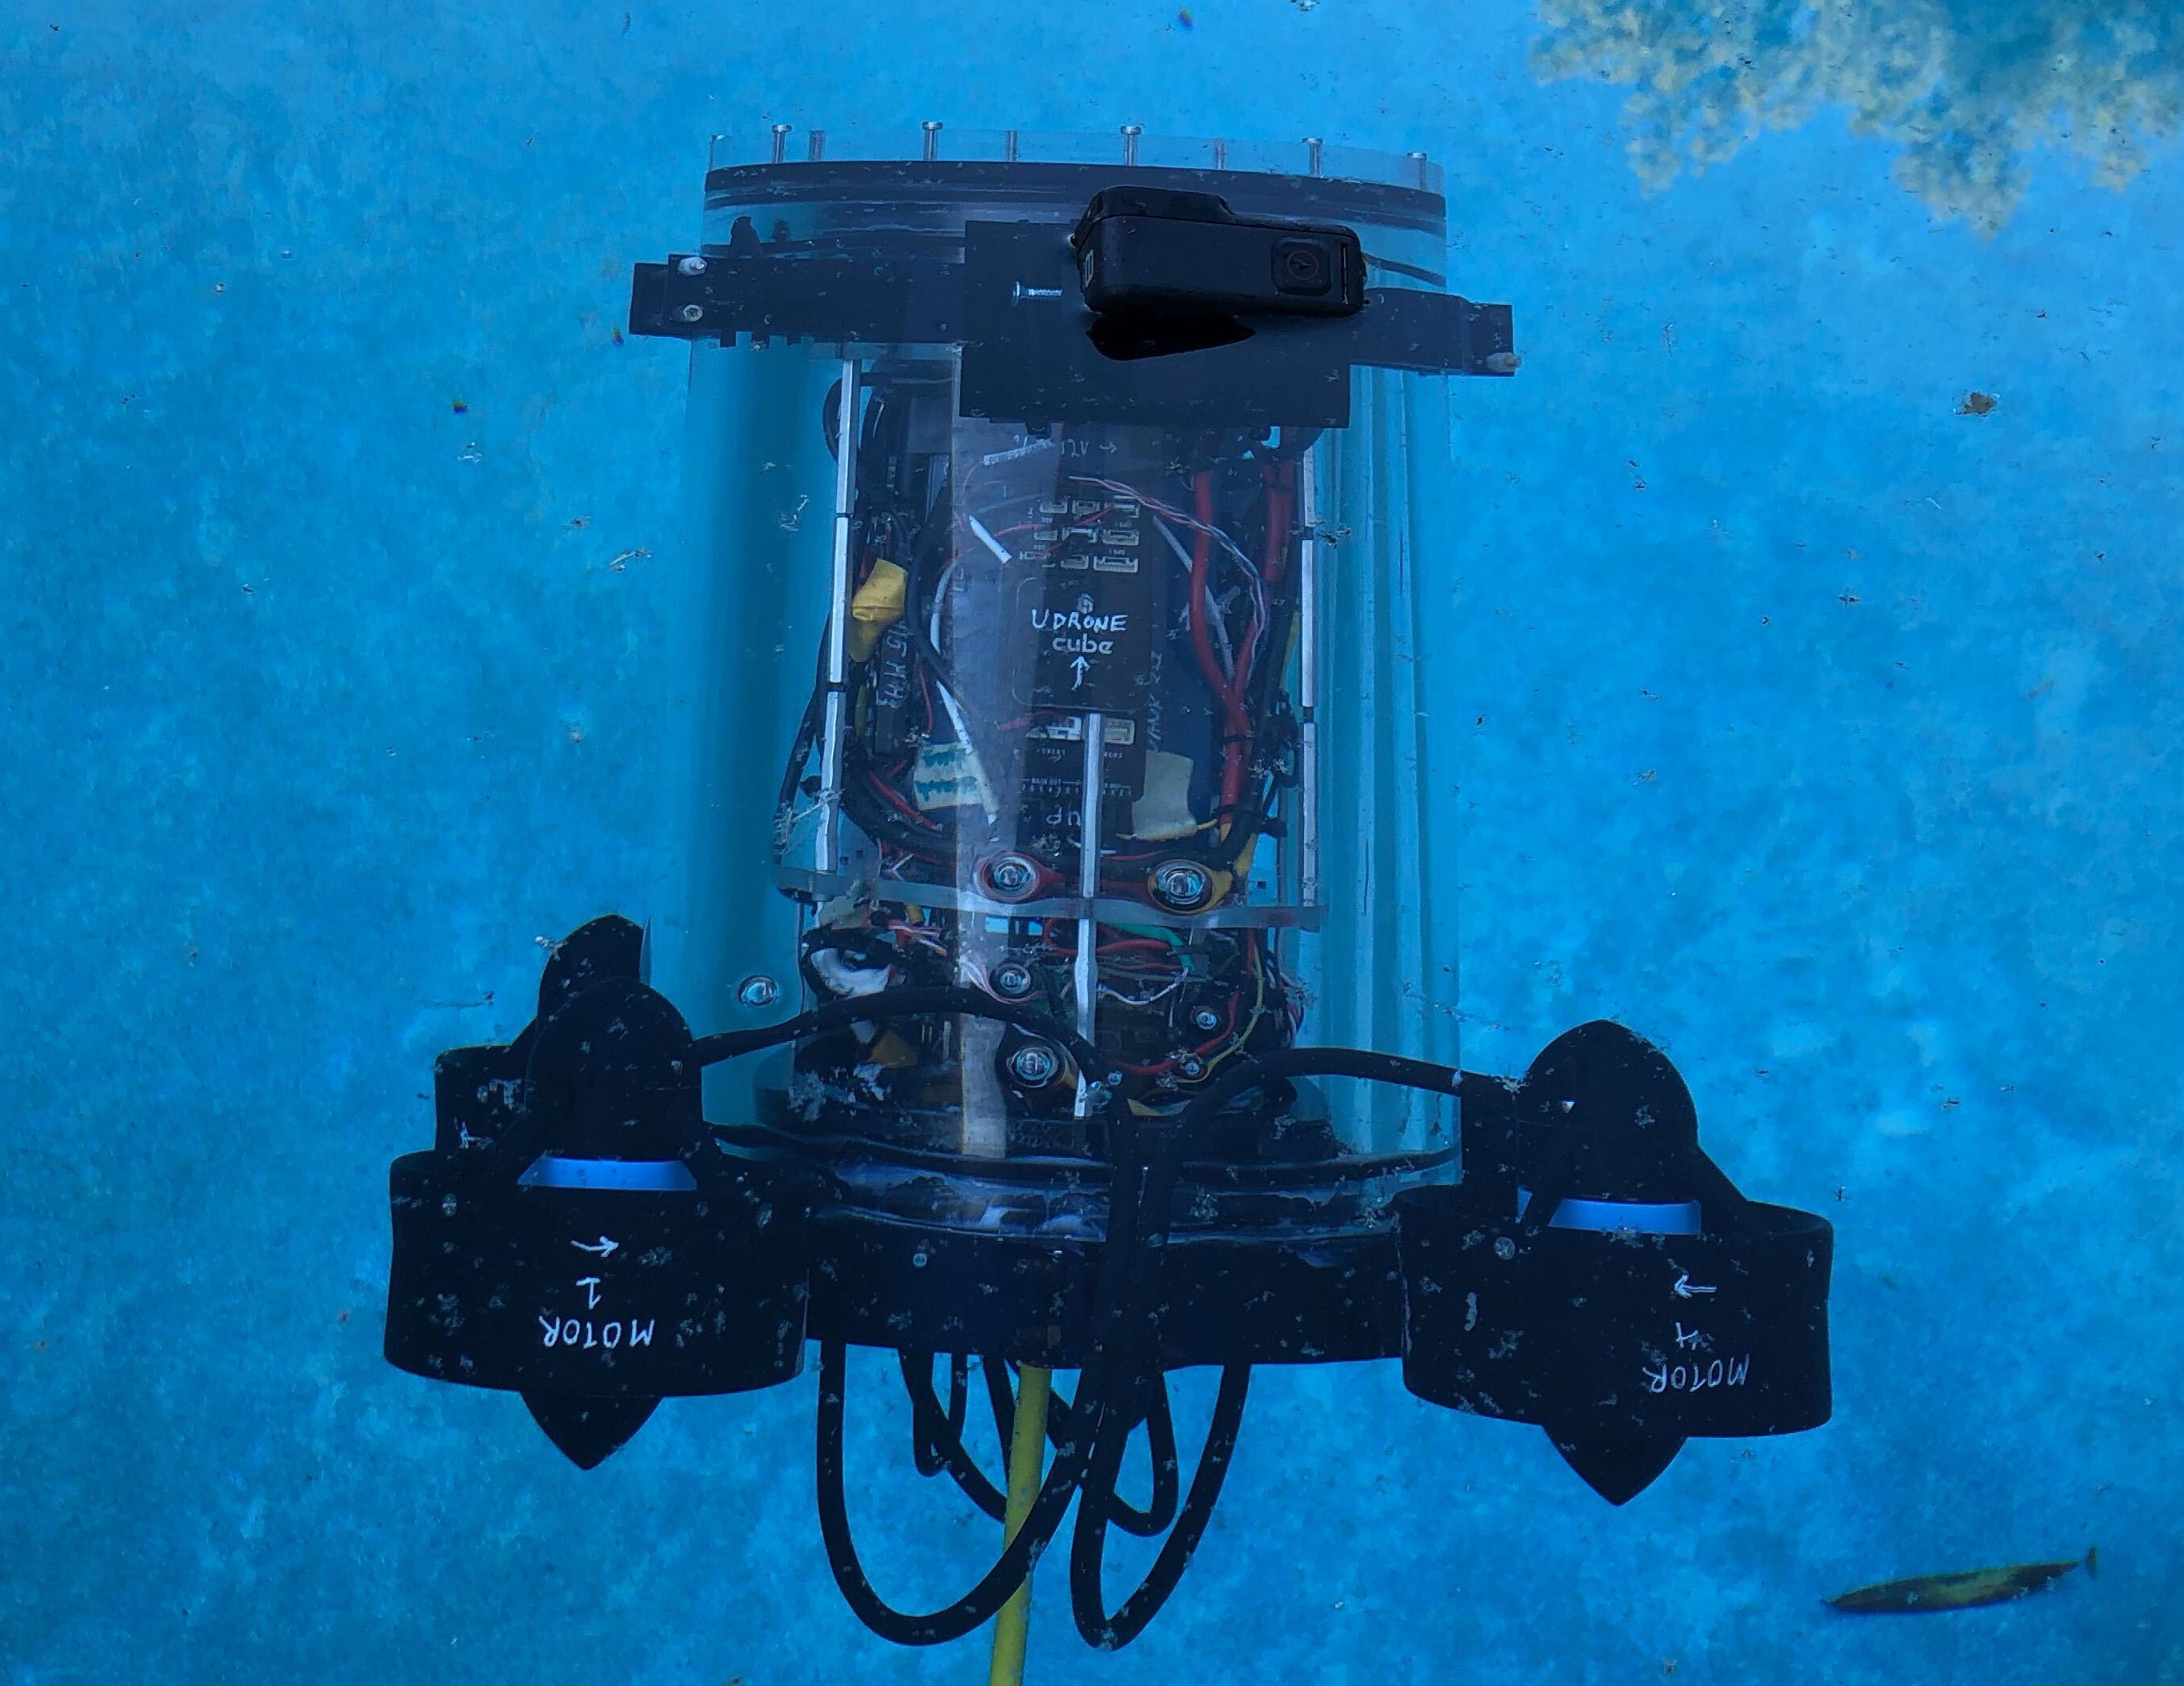
\includegraphics[width=\maxwidth{\textwidth}]{img/drone_pool2.jpg}
\caption{uDrone in Pool Test}
\legend{\emph{Source}: Photo courtesy of Jnaneshwar Das, used with permission.}
\label{pool}
\end{figure}
For all these reasons, the DREAMS lab decided to build a new, customized autonomous underwater vehicle. Based on a motor configuration that mimics that of a quad-rotor aerial vehicle, colloquially referred to as "drones", this vehicle was named the uDrone. This chapter will outline the motivation for developing the uDrone. Subsequent chapters will go through the background of the underwater vehicle world before the uDrone, the technical details of the uDrone system and its development, and a detailed mathematical model of the vehicle dynamics. Lastly, two methods of autonomously controlling the uDrone are explained, evaluated, and compared. 

\section{Thesis Statement}
\begin{center}
    \emph{An autonomous underwater drone testbed that leverages state of the art avionics and machine vision algorithms will enable safe, cost-effective, and time-efficient coral reef exploration and monitoring at a global scale.}
\end{center}
This statement can be broken down to better understand the project goals. Autonomous is defined as being able to operate without direct human control and supervision. Underwater drone is the vehicle itself, emphasizing the setting it is meant to explore. Testbed is a set of software and simulation tools to enable rapid development and testing. State of the are avionics refers to control methodologies and algorithms developed for quad-rotor aerial drones that can be applied to this project. Machine vision algorithms will be used to create and understanding for the vehicle of its surroundings, which is key to enabling autonomy. The uDrone seeks to be safer and less time consuming than the diving being done for related research currently while meeting the budgetary goals. And reef exploration and monitoring is the vehicles ultimate goal and purpose; all the other elements combine to enable this final goal. 

\section{Science Motivation}

GDCS has several ways of obtaining large quantities of imaging data. They contract with Planet satellites and fly an aeroplane fitted with special equipment, known as the Global Airborne Observatory (GAO). These methods have been used to do extensive research on South American rain forests whereas coral reefs are the current "frontier" of research for the GAO. Better imaging and monitoring of coral reefs will enhance researchers understanding of the effects of climate change on reefs and allow for more detailed coral models to be created. 

The immediate goal is to develop a three-dimensional structure of coral reefs that contains full spectral data, from 400 to 800 nm \parencite{gdcs_sat}. This goal is made more difficult by the inherently complex physics of light moving through water. Several methods have been explored to essentially "see through" the water and retrieve the data from the coral alone. In one approach, the inherent properties of the water are used to calculate the effects of the water on the light spectra moving through it \parencite{gdcs_gao}. In another, bottom reflectance data is collected by scuba divers with specialized equipment and used to calibrate the data from satellites \parencite{gdcs_ads}. 

This last method necessitates a human operating in a potentially dangerous environment to collect data. Specifically, Dr. Greg Asner, head of GDCS would use a ADS HandHeld 2 Spectrometer attached to a diver propulsion vehicle (DPV) to collect samples. These data collection trips would last up to four hours and very few researchers have the technical diving capability or constitution to complete them. This was the initial motivation for the uDrone project. Figure \ref{asner} shows the DPV and its use on the reef. 

\begin{figure}[h]
\centering
\subfigure{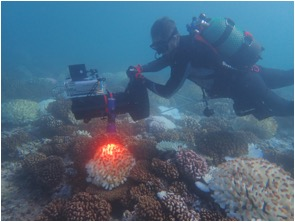
\includegraphics[width=0.49\linewidth]{img/asner.jpeg}}
\subfigure{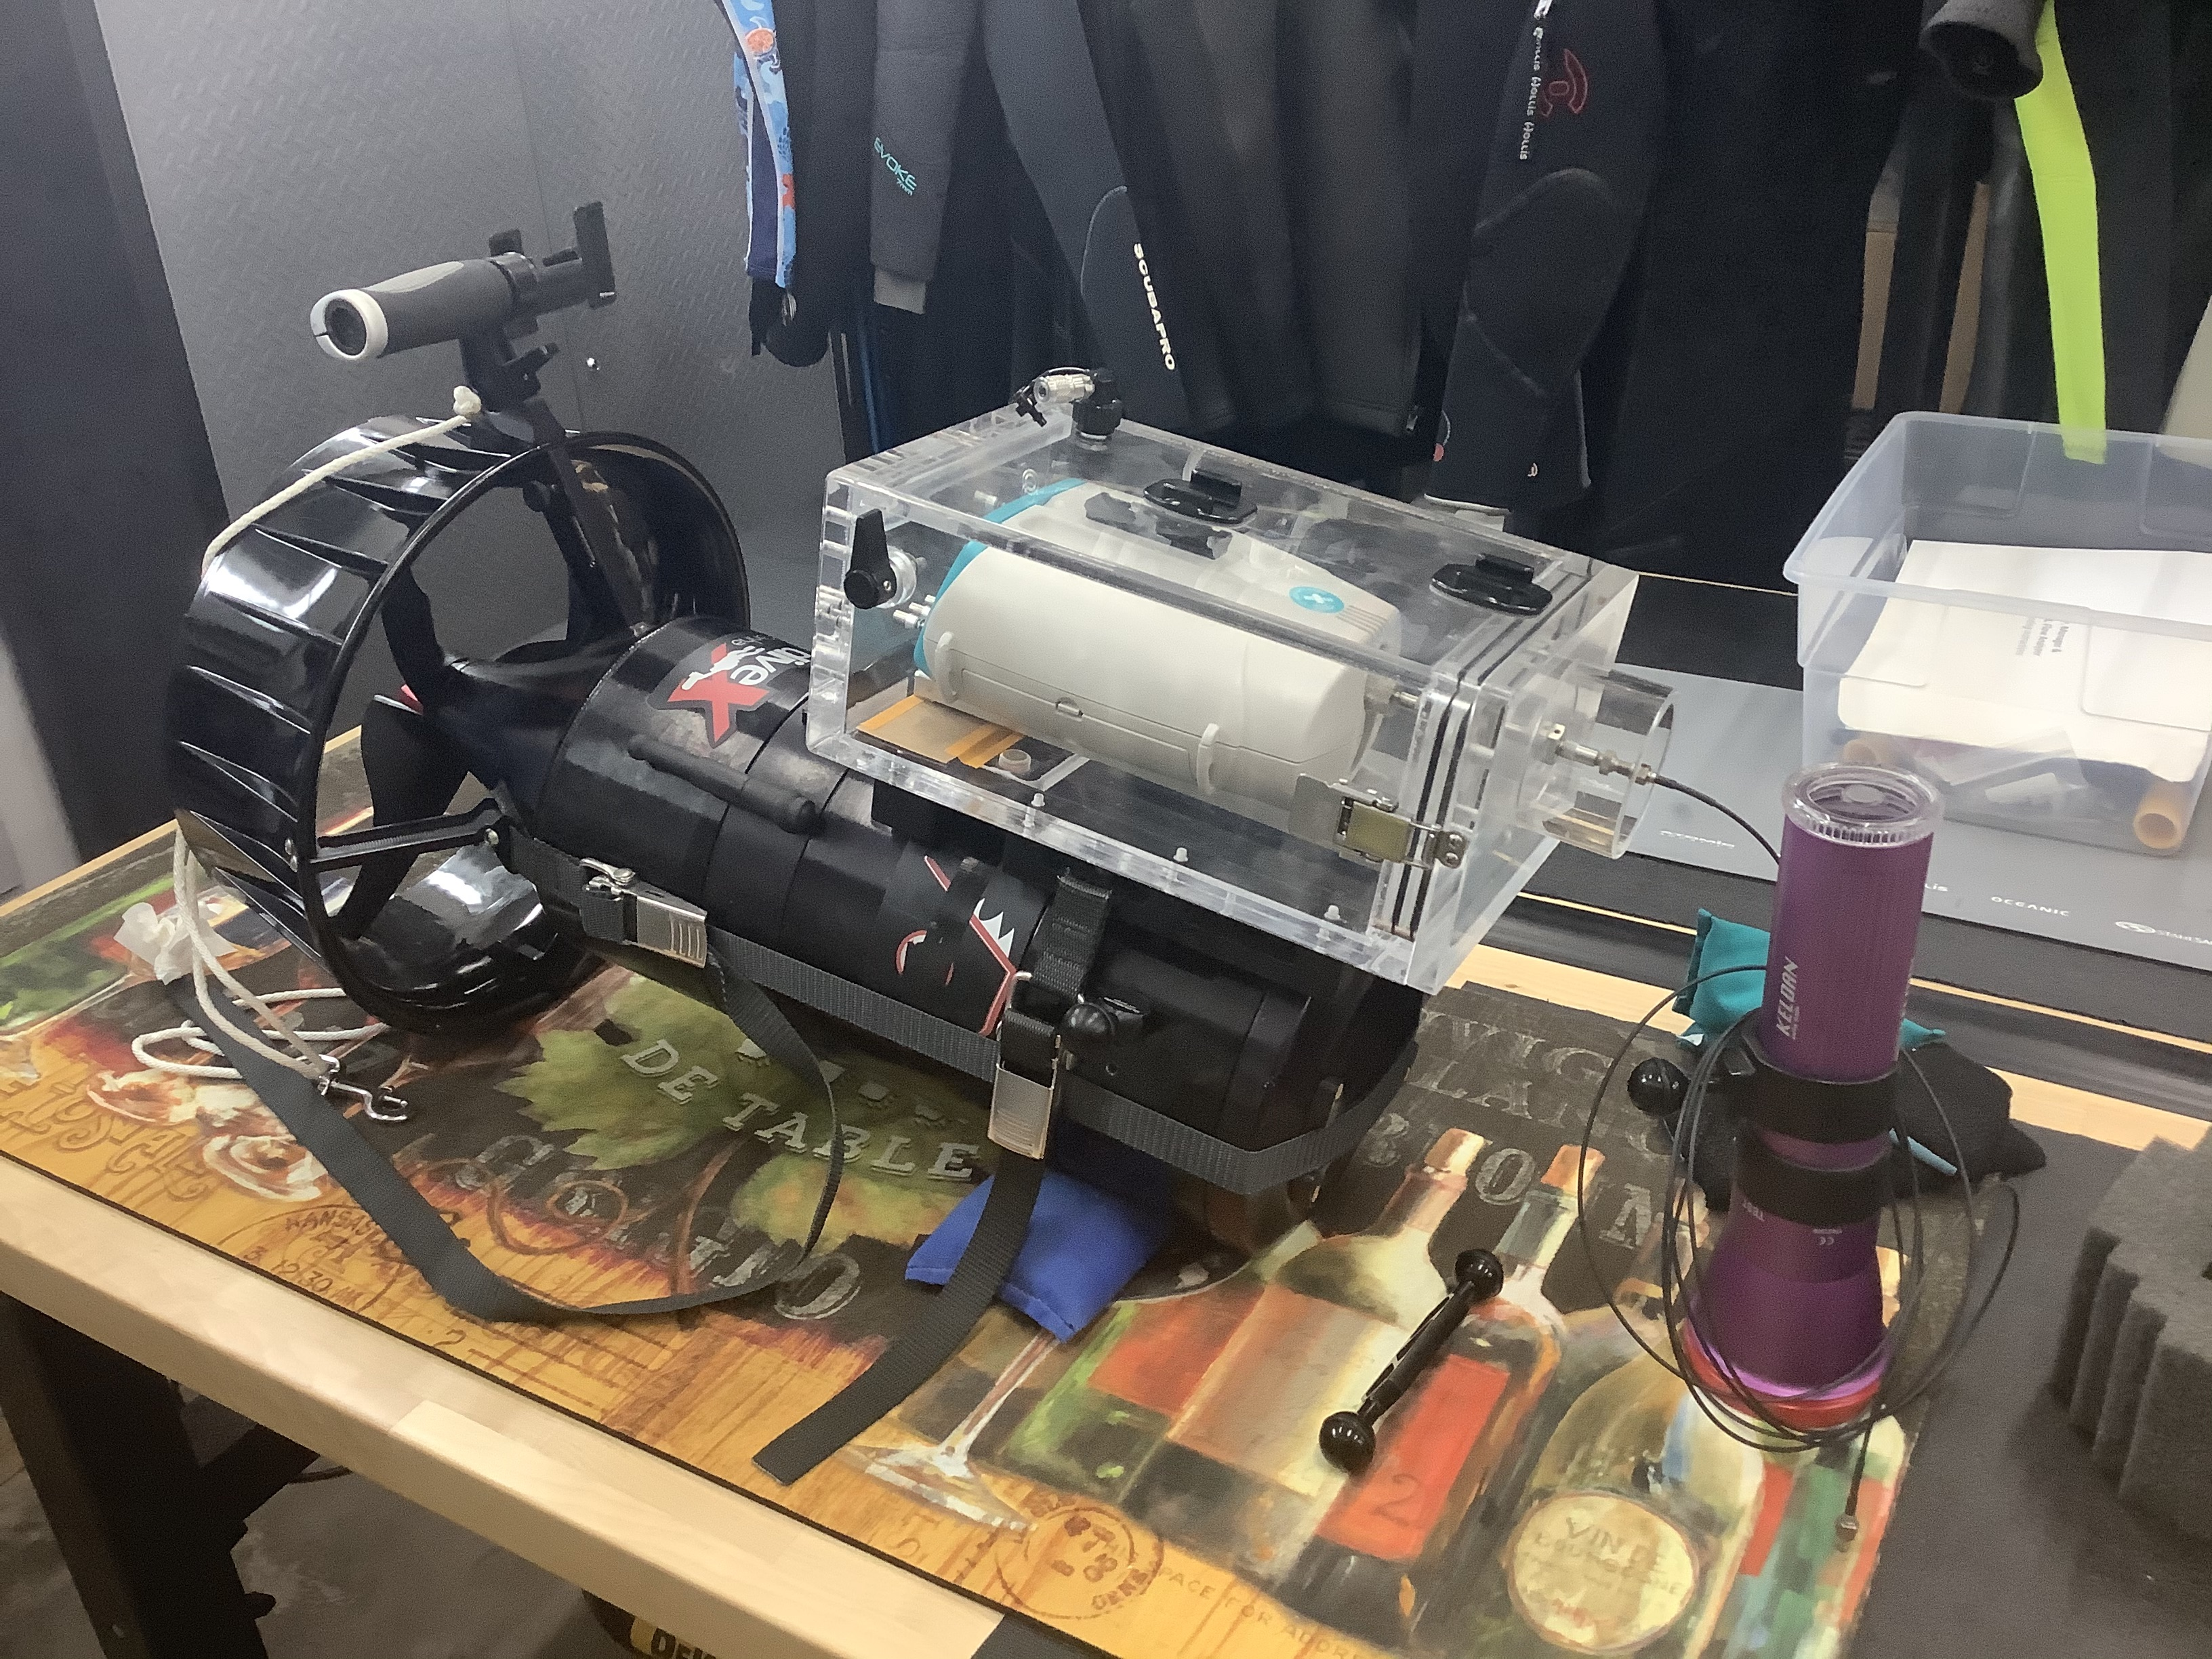
\includegraphics[width=0.49\linewidth]{img/DPV.jpg}}
\caption[DPV Deployed to Collect Reef Data]{Dr. Greg Anser using a DPV for collecting data (left) and the DPV out of water with the sensor attached}
\legend{\emph{Source}: Left photos courtesy of Greg Asner, used with permission.}
\label{asner}
\end{figure}

The risk of death from scuba diving is low, with an estimated annual death rate of 2 deaths per 100,000 recreational scuba divers in the United States. Many of these deaths are due to cardiovascular health and diver errors \parencite{dan}. These risks are mitigated in the scientific diving community by the increased requirements set out by the American Association of Underwater Scientists (AAUS), which require additional training and medical checks \parencite{aaus}. ASU and all associated labs follow these requirements for diving activities.

Dive injury, however, is significantly more common than fatality, with an estimated 15 occurrences per 10,000 dives. While there are many potential avenues for dive injury, including interactions with the marine environment, barotrauma, and gas contamination, one ailment in particular can strike divers at any skill level and is particularly exacerbated by long and repeat dives. This is decompression sickness. Decompression sickness is the second most common type of dive injury, accounting for 27\% of all dive injuries according, to the Divers Alert Network (DAN), the world's largest scuba diving safety association. (Barotrauma is the most common accounting for 41\% of injuries). 

Decompression sickness, or DCS, is caused when gas bubbles absorbed by body tissue at higher pressures underwater are not able to properly “off-gas” or reabsorb. This can cause bubbles to form in various regions of the body. Most commonly this occurs in joints or tissue which can impair motor function and have permanent effects. In some cases a bubble can form in the circulatory system, blocking blood flow, which can be fatal \parencite{dcs}.

In order to reduce the risk of DCS while diving, scuba divers use tools to monitor the dissolved gasses in their system. Historically, this has been done with tables before and after a dive but most modern divers use a dive computer which tracks their gas absorption. This risk can also be mitigated for especially deep or long dives by mixing inert gasses into the breathable air in order to limit the amount of any one gas that gets absorbed.

An AUV, such as the uDrone, can be deployed to totally eliminate the health risks associated with human-based coral reef data collection. This also opens up the possibility of significantly more data to be collected for the existing GDCS projects, along with finding new opportunities for collecting and using reef data. For example, researchers at the University of Hawaii, Hilo are collecting detailed imaging data of coral reefs and using them to create three-dimensional reconstructions of the reef. These reconstructions are then incorporated into other data sets for ecological monitoring \parencite{burns}. The uDrone would allow for more data to be collected with less human health risk as it replaces divers who collect data. 

\section{Engineering Motivation}
While the scientific need inspired its initial creation, the uDrone is useful beyond these specific implementations. It is quickly becoming a testbed for innovation in autonomous underwater navigation within the DREAMS Lab. One thesis has already been written leveraging the system for multi-robot coordination and several others are in the works at this time.

The development of a testbed starts with two parallel tracks: hardware development and software in the loop (SITL) simulation. In the hardware development phase the needs of the vehicle are determined, currently available hardware is specified and sourced, and the vehicle itself is put together. SITL simulation is a method of simulation where all elements of the vehicle are simulated, including the flight controller, the internal computation, the vehicle itself, and the world in which it operates. These tracts combine to a third step: hardware in the loop simulation. In this step the vehicle motion is still simulated in a virtual world, but the flight controller and internal CPU of the actual vehicle interact with this simulation. This step leads to the final step in the chain, which is real world deployment.

\begin{figure}[ht]
    \centering
    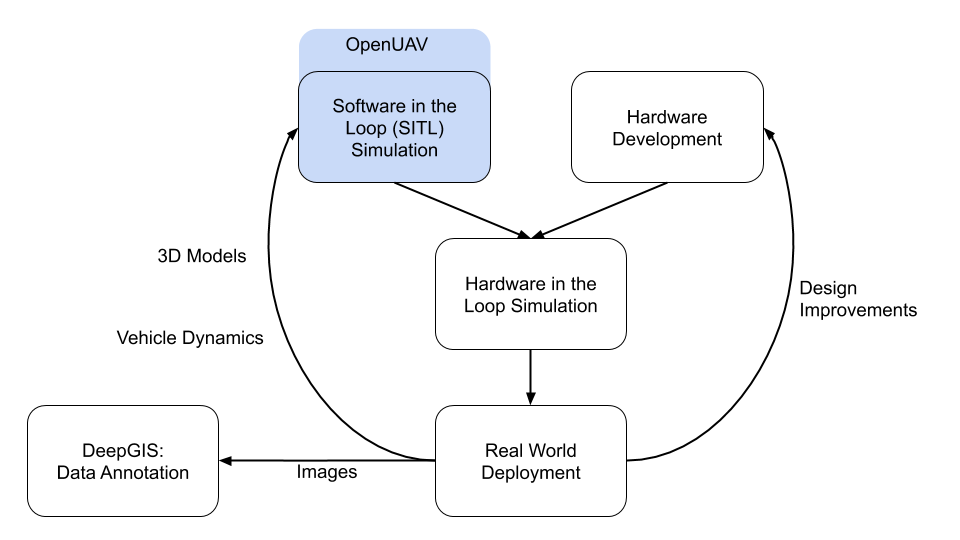
\includegraphics[width=\maxwidth{\textwidth}]{img/testbed.png}
    \caption{The testbed steps and cycle of development}
    \label{testbed}
\end{figure}

This process, illustrated in Figure \ref{testbed}, is not a straight path but a cycle. The real world deployment generates leanings which are put back into the first steps to improve the uDrone. Design improvements are gathered every time the vehicle is put together or deployed. In fact, the vehicle pictured in Figure \ref{3ways} is the third iteration of the internal structure to hold the equipment. The real world deployments also generate more data about the vehicle's dynamics and images collected can be used to create additional 3D reef models. These can be used to make the simulation environment more realistic and accurate. This also feeds nicely into other DREAMS lab projects. The SITL simulation has become part of the OpenUAV stack, a tool for rapid prototyping and remote working. And the images collected from deployment can be fed into DeepGIS, a tool for annotating data for machine learning. 

% This testbed has several benefits for innovation:
% \begin{itemize}
%     \item An existing simulation environment allows for rapid software prototyping. Robotic software developers can focus on writing code, not building simulation environments, and configuring vehicles. 
%     \item Transitioning from simulation to reality is made easier.
%     \item The simulation can be continuously updated as more real-life trials are run with the vehicle. 
% \end{itemize}
    
% Additionally, building a vehicle from scratch is less expensive and easier to maintain than a purchased vehicle. This is because all the components are either off the shelf or built in house. This allows for the efficient acquisition of backup parts. The DREAMS lab team, having intimate knowledge of the vehicle, can troubleshoot and perform maintenance without outside help. Since the cost is low, it is possible to build multiple vehicles and perform swarm activities.

% A good example of similar platform leading to innovation can be seen at Greg Dudek’s Lab at McGill. They AQUA robot was built over 10 years ago and students are still using it today for research \parencite{aqua}. The work has transitioned from hardware to computer vision and autonomous navigation. For example, using this platform a new vision based underwater navigation tool called Nav2Goal was created. In this, the underwater vehicle moves to a goal defined by the user. Along the way, it not only avoids obstacles but also takes paths that bring it near to areas of greater interest. This is particularly useful in coral reefs when a vehicle can decide to follow a path along a coral reef instead of a sandy bottom on its way to its goal \parencite{rtcv}.


% \subsection{Personal Motivation}
% My interest in building the uDrone with the DREAMS Lab at ASU started during my first semester as a Master’s Student in Robotics and Autonomous Systems. I took Prof. Das’ Exploration Systems Design class. My final project for this class was the construction of a boat to start the lab’s stable of aquatic vehicles. For this project, I handled all aspects of construction, system design, assembly, and configuration. This was my first intro to building an autonomous system from the ground up. The boat has been used for several projects in our lab and Prof. Das’ class. After successfully building and deploying this vehicle, and based on my personal experience with scuba diving, I was invited to create the system for an autonomous underwater drone for the lab.

% I started scuba diving at the age of 11. By 15 I had over 100 dives under my belt and was trained as a Rescue Scuba Diver. At 19 I became a certified Scuba instructor. During my undergrad at the University of Michigan, I was one of the leaders of the Human Powered Submarine Team. We designed, built, and raced a submarine powered by a scuba diver inside pedaling bicycle pedals. After school, I volunteered as a Scuba diver at the Shedd Aquarium in Chicago. I proposed to my wife underwater. This is all to say: I have been personally interested in Scuba diving and reef conservation for a very long time. This made me the perfect candidate to leverage my skills in robotics to design a vehicle to help divers get more done.

% Beyond the robotic boat mentioned above, I have a history of building platforms and technology that enable others to achieve more. My first job out of college was at a data center where I developed a novel containerized data center product. This allowed for a drastic decrease in the construction time of data centers while increasing energy efficiency and reliability. Later, I founded several startups with the aim of creating tools and experiences to help. Mm y last and most successful startup created a special type of event that made it easier for strangers to meet and make friends. And immediately before joining ASU for my Master’s, I built a platform for a mortgage company that gave more transparency and power to borrowers in the loan process. This is all to say I am very passionate about building platforms and systems that enable innovation. This, along with the diving, drew me to the challenge of developing the uDrone. 

                     %<Insert your chapters here; I recommend to use
\chapter{Background}

There are many unique challenges to building autonomous vehicles for underwater environments. And, several other university labs and organizations have build vehicles for aquatic exploration. This section will discuss these challenges and several of the most relevant vehicles. 

\section{Challenges of Underwater}
Working in underwater environments presents a number of challenges not experienced by aerial, ground, or surface vehicles. These include physical challenges, difficulty of communication, and lack of global positioning systems. 
\subsection{Physical Challenges}
First and foremost is the need to seal the vehicle for water and pressure. The uDrone will need to maintain a watertight seal down to 30m of water. This is made more challenging by the need to have some components exterior to the enclosure which houses the electronics, necessitating the creation of watertight pass-throughs. As the vehicle goes to deeper depths this becomes increasingly harder. Every 10m of water adds an additional atmosphere of pressure to the vehicle. This pressure causes two problems. First, enclosures must be strong enough to resist the force of the pressure change and not fail structurally. Second, o-rings and other seals shrink under pressure, which can lead to leaks. 

In order to achieve this, the uDrone uses a Blue Robotics enclosure to keep the electronics dry inside. In order to handle the cable pass-throughs, and o-ring sealed pass-through is attached to the rear of the enclosure and then the potting compound is used to seal the area between the cable and pass-through. 

An underwater vehicle also has to manage its buoyancy. If the vehicle is too heavy or too light it will end up moving through the water column at an angle, increasing drag and decreasing efficiency. Additionally, if the centers of buoyancy and mass do not line up then there will be a moment acting on the vehicle, complicating modeling and control. While this presents challenges, it can also lead to opportunities. By creating a vehicle that is slightly positively buoyant or by having a mechanism that allows a vehicle to drop ballast, a vehicle will float and can be recovered in the event of failure. Since the main camera on the uDrone is front-facing, the center of buoyancy can be set slightly behind the center of gravity. This will cause it to point down when hovering, but in motion, the thrusters can compensate for the moment. 

Many autonomous vehicles are able to simplify certain aspects of the model. For example, a vehicle moving through the air does not need to worry about added mass from the layer of air near the vehicle surface. In fact, air drag is often ignored unless a drone is moving at high speeds. This is not possible underwater due to the greater viscosity and density of water compared to air. In order to get reliable system modeling, expensive and complicated fluid dynamic software must be used. Since this is often impractical for applications such as the uDrone, the values for added mass and drag are often estimated and then verified experimentally. 

Similar to the effects of wind on an aerial vehicle, underwater vehicles must be able to compensate for currents. This is made more challenging as the speed of the vehicle cannot be verified by GPS. Instead, visual odometry must be used to determine the effects of current on the vehicle and aid in compensation. 

\subsection{Communication Challenges}
WiFi or radio signals do not penetrate to useful depths underwater. Radio waves in the MHz or higher frequency range typically penetrate less than 1 meter underwater. Since the radio controllers used on drones communicate at 900 MHz and WiFi uses 2.4 GHz or 5 GHz, none of these are viable communication options. 

Optimal communication is possible but is limited by line of sight and water column turbidity \parencite{light-coms}. Optimal communication has been implemented in a simulation for the uDrone, where it follows a boat that has a visual marker mounted underneath. This is reasonable for some use cases of the uDrone, but cannot be relied on for all scenarios.

% https://www.hydromea.com/underwater-wireless-communication/
The most common method of real-time communication with underwater vehicles is via a tether. This allows for fast and reliable connections but limits the movement of the vehicle based on cable length and cable management. While the uDrone is capable of functioning with a cable for testing purposes, it is designed to operate without one. 

The only reliable method of wireless underwater communication is via acoustic transponders. However, these devices tend to be large, expensive, and power-hungry. While one day it might be useful to have wireless acoustic communications at specific sites of uDrone deployment, it is not practical in the initial use case.

\subsection{Global Positioning and Navigation Challenges}
GPS satellites transmit data at high frequencies, in the GHz range. For this reason, traditional, satellite-based GPS is not practical for use underwater. The uDrone is still outfitted with GPS so it can determine its location on the surface, but it cannot rely on this as a method of localization while underwater.

It is possible to use acoustic signals to localize an underwater vehicle. This requires three or more surface-based acoustic broadcasters. An underwater vehicle can then triangulate between these sources in order to determine its position relative to the sources. This is basically the equivalent to creating an underwater GPS system. While it is possible that this could be implemented at some operational sites in the future, it is not practical to build in the beginning and is therefore not a reliable way for the uDrone to localize.

Due to the lack of GPS, the uDrone must use visual and inertial based odometry to determine its location. LIDAR, which is the measurement tool of choice of most aerial and land-based robots, is severely limited underwater for two reasons. First, lower frequency light is absorbed quickly underwater, and since most LIDARs use these lower frequencies, the range is severely limited. Second, murky water greatly limits the ability of light to pass through water, and since it is very common to have many dissolved particles in the water column this makes LIDAR inaccurate. Therefore, the best type of sensor to measure distance underwater is with an echo-sounder. 

Another tool typically used by land-based robotics to understand their surroundings is using depth cameras. There are two main types of depth cameras: stereo and infrared. Stereo cameras calculate the pixel depth of an image by looking at the difference in location between the images from two cameras placed a known distance apart. Infrared cameras work by projecting a pattern in infrared light onto surfaces and using the deformations to calculate distance. Since lower frequency lights, such as red and infrared, are absorbed most quickly by water, infrared depth cameras do not work well underwater. For this reason, a stereo camera is the most practical type of depth camera for use underwater. 

\section{Previous Work}
Existing Autonomous Underwater Vehicles (AUVs) and Remote Operate Vehicles (ROVs) tend to fall into 2 categories: Flight style and hover style. Flight style vehicles are similar to torpedoes. They typically have long, cylindrical bodies with a single thruster at the rear and control surfaces to control roll, pitch, and yaw while moving. These vehicles are typically used in the open ocean to complete larger area surveys, which necessitates their long range and higher speeds. The trade offs for speed, endurance, and range are less controllability, agility, and precision. Hover style vehicles have nearly opposite abilities. They are typically box shaped with multiple thrusters in various directions allowing for precise movement in any direction. Due to the challenge of controlling these highly maneuverable vehicles, they are typically ROVs, meaning there is a pilot on the surface connected via a tether and they are not autonomous. 

In this chapter I will present four vehicles, one each in the flight and hover style and then two in a newer category of underwater vehicle, called hydrobatic. Hydrobatic vehicles are both fast and agile, balancing the trade-offs between the range and speed or flight style vehicles and the maneuverability of hover style vehicles. The two hydrobatic vehicles presented here served as inspiration for the uDrone. This section is not meant to be a comprehensive review of underwater vehicles. Instead, it will serve to show some examples and give some background of the research that inspired the uDrone. 

\subsection{HippoCampus $\mu$UAV}
The HippoCampus micro underwater vehicle was developed at the Institute of Mechanics and Ocean Engineering, Hamburg University of Technology in Germany. This small, agile, and inexpensive vehicle was developed for use in swarms. Similar to the uDrone thruster configuration, the HippoCampus drew on inspiration from multi-rotor aerial vehicles to develop a four propeller design \parencite{hipp1}. In fact, the open-source code developed for this vehicle has been a huge help in designing gazebo simulations and PX4 controllers for the uDrone. Robust models were derived for the HippoCampus which were used to show its ability to function as a submerged Furuta Pendulum \parencite{hipp_pen}. Designed to be inexpensive and work in swarms, the HippoCampus has limited capacity for sensors. It uses a gyroscope, compass, and depth sensor, but does not make room for any visual or sonar sensors.

\subsection{AQUA: an Aquatic Walking Robot}

The AQUA robot was developed over 10 years ago by the  Mobile Robotics Lab at McGill University. It is based on the RHex hexapod robot. Its original intent was to create an amphibious robot that could transition from walking on land to swimming in water. Instead of thrusters, which are used by the majority of underwater vehicles, the AQUA robot uses six fins to propel itself through the water \parencite{aqua}. More recently, this platform has been used with an on board GPU in order to handle vision based navigation \parencite{MandersonGPU}.

The AQUA, along with its simulation environment, is a good example of an underwater robotic testbed leading to innovation. The work has transitioned from hardware to computer vision and autonomous navigation. For example, using this system a new vision based underwater navigation tool called Nav2Goal was created. In this, the underwater vehicle moves to a goal defined by the user. Along the way, it not only avoids obstacles but also takes paths that bring it near to areas of greater interest. This is particularly useful in coral reefs when a vehicle can decide to follow a path along a coral reef instead of a sandy bottom on its way to its goal \parencite{manderson2020visionbased}.

While this vehicle satisfies most of the requirements of the uDrone project, it was mainly developed as a research vehicle and for amphibious implementations, making it not ideally suited to the project needs. 

\subsection{Light Autonomous Underwater Vehicle}
The Light Autonomous Underwater Vehicle (LAUV) was developed in 2012 by the Laboratório de Sistemas e Tecnologia Subaquática (LSTS) at the Universidade do Porto in Protugal and is manufactured by OceanScan Marine Systems \& Technology. This vehicle was designed to be small enough to be carried by one person while still having full capabilities for scientific and defence surveys. It is built in the ‘flight’ or ‘torpedo’ style of underwater vehicle, having a long cylindrical body with a single thruster at the rear and control surfaces to control roll, pitch, and yaw while moving. The LAUV has an endurance of 6-8 hours at a speed of 1.4m/s, which would satisfy the same needs as the uDrone \parencite{lauv}. However, due to the flight style design it would not be able to reliably and precisely follow the terrain of the reef as necessitated by this project.

\subsection{Blue Robotics ROV2}
There are many ROVs exploiting the oceans, from the 2,400 kg ROV Minerva used for deep ocean research \parencite{minerva}, to the 3.4 kg Sofar Trident consumer underwater drone \parencite{sofar}. Because it uses many similar hardware components along with an open source software stack, the Blue Robotics ROV2 will be highlighted here. This vehicle is sold as a kit by Blue Robotics, utilizing many of its components. It is meant for both recreational enthusiasts and small scale research. The vehicle is from the surface via a tether. Onboard, it houses a PixHawk flight controller running ArduPilot, an alternative to PX4. Additionally, cameras, echo sounders, and other sensors can be added to the vehicle. It has a maximum speed of 1.5 m/s and a battery life of about 2 hours \parencite{bluerov}.

The Blue Robotics ROV2 has been used for autonomous underwater navigation experiments. One such set of experiments, conducted at the French-Mexican Laboratory on Computer Science and Control. The authors used the tether of the ROV2 to retrieve sensor data from underwater. This data was processed on a remote ground station and then sent back to the vehicle, again via the tether. The whole system operated with ROS and the MAVROS interface to ArduPilot. This allowed for real time and off board computer vision based autonomy \parencite{rtcv}.

\chapter{Technical details of uDrone System} \label{system}
This section will list the requirements for the uDrone system along with the chosen hardware components and software tools used to meet them.
\section{System Requirements}
Based on the science needs and goals of building a testbed, several design requirements emerged.
\subsection{Science Requirements}
\begin{itemize}
    \item Maintain a constant speed of 1 m/s.
    \item Maintain a constant distance from the reef, ideally between 30 and 100 cm.
    \item Know the exact distance to the reef to calibrate spectrography readings.
    \item Operate for at least 4 hours.
    \item Be able to carry the necessary spectrography equipment and light source.
    % \item “Field spectra were measured using an ASD HandHeldPro-2 spectrometer with an underwater housing and tungsten halogen light source at a distance of 10 cm from the benthic targets (live coral, bleached coral, etc.) (Appendix A, Figure A2). (cite: Li sensitivity…)
    \item Travel fully autonomously, with no tether or human control.
    \item Maintain a straight line path underwater.
    \item GPS tag the start and end locations in order to estimate the exact locations of all measurements in-situ.
    \item Be deployed and retrieved by one or two people from the shore or a small boat. 
\end{itemize}

\subsection{Testbed Requirements}
\begin{itemize}
    \item Use ROS and PX4 as open source frameworks.
    \item GPU to allow for on board machine learning and neural networks.
    \item Sensors to generate local awareness for navigation.
    \item Cost less than \$10,000.
    \item Easy access to internal components.
    \item Each component replaceable or upgradable.
    \item Code can be tested in a robust simulation environment.
\end{itemize}

\begin{figure}[h]
\centering
\subfigure{\includegraphics[width=0.35\linewidth]{img/side.png}}
\subfigure{\includegraphics[width=0.28\linewidth]{img/front.png}}
\subfigure{\includegraphics[width=0.34\linewidth]{img/ortho.png}}
\caption[Side, front, and orthogonal view of the uDrone]{Side (left), front (center), and orthogonal (right) view of the uDrone}
\label{3ways}
\end{figure}

\section{Hardware Components}
The hardware components were chosen to be easy to obtain and mimic the construction of autonomous aerial vehicles as much as possible. The  physical and logical connections of the uDrone system is diagramed in Figure \ref{system_diagram}. In this diagram the blue boxes represent physical components, the red boxes represent software frameworks, the solid lines represent physical connections, and the dashed lines represent logical connections. The specific components listed here are discussed in the remainder of this chapter. 

\begin{figure}[h]
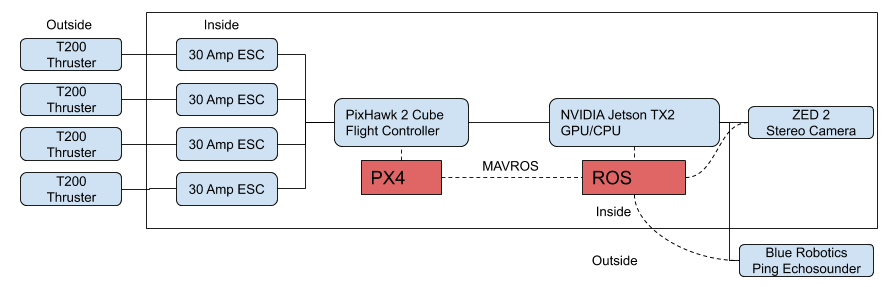
\includegraphics[width=\maxwidth{\textwidth}]{img/uDrone System Diagram.png}
\caption{uDrone System Diagram}
\label{system_diagram}
% \legend{\emph{Source}: \iftoggle{usebiblatex}{\textcite{krishnappa_adult_2012}}{\citet{krishnappa_adult_2012}}}% See: https://upload.wikimedia.org/wikipedia/commons/8/89/Antidorcas_marsupialis%2C_male_%28Etosha%2C_2012%29.jpg
% \legend{\emph{Note}: Here is a note that is especially long to show what happens when it extends to more than one line.}
\end{figure}



\subsection{Blue Robotics T200 Thrusters}
% https://bluerobotics.com/store/thrusters/t100-t200-thrusters/t200-thruster/
% https://discuss.bluerobotics.com/t/t200-high-voltage-behavior/94/4 (lifespan)

Blue Robotics is a leading source for marine robotics components. Arising from a kickstarter in 2014, they are DREAMS Lab’s preferred vendor for many components. Their thrusters fit the uDrone’s needs quite well, including their size, power usage, thrust capabilities, depth limits, and price. Additionally, as these are sold commercially it is very easy to have spares and order more on short notice. Given how perfectly these thrusters fit the requirements, no other thruster was seriously considered. One potential drawback to these thrusters is the expected lifetime of 600-1000 hours \parencite{t200}. While for some long range missions this would be a problem, with a mission time of only a few hours this poses no risks to the uDrone. 

The thrusters are controlled via a 30 amp electronic speed controller (ESC). This device modulates the power to the device based on pulse width modulation (PWM) signals it receives from the flight controller. 

\subsection{PixHawk 2 Cube Black}

% https://docs.px4.io/v1.9.0/en/flight\_controller/pixhawk-2.html
% http://www.proficnc.com/all-products/31-pixhawk2-suite.html

The DREAMS Lab uses PixHawk flight controllers for most aerial and aquatic robotics applications. Due to the experience and expertise with this piece of equipment, the same type of flight controller is used for the uDrone. The cube was chosen over newer PixHawks, like the PixHawk 4 mini, because it is more widely used in the PX4 community and the smaller size was not needed for the uDrone implementation.

The PixHawk 2 Cube runs PX4 on the NuttX operating system. It has multiple built-in three-axis gyroscopes, accelerometers, and magnetometers along with barometers, forming redundant internal measurement units (IMUs). It communicates with the on-board computer via MAVLINK messages over a serial connection. These messages are generated on the on-board computer from the MAVROS package. The PixHawk is able to control the motors via PWM outputs. 

These PixHawk devices typically run either PX4 or ArduPilot. Due to DREAMS Lab’s expertise, along with the related work being done, PX4 is used for the uDrone. The PX4 software has several different flight modes, including position, altitude, acrobatic, and manual control. The uDrone uses the acrobatic mode controlled via the on-board computer. In this mode the controller receives the desired orientation or angular rate along with a thrust value. Utilizing the internal IMUs, a built in PID controller takes these inputs and sends the desired PWM command to each motor \parencite{px4_pixhawk}. 

% \begin{itemize}
%     \item An STM32F427 Rev 3 Flight management unit
%     \item An STM32F100 I/O processor with pass through capabilities for failsafe
%     \item 3 IMU's
%     \item 1 Fixed 10 Axis IMU on the main Main board
%     \item 2 Vibration Isolated and heat controlled 9DOF IMU's and an isolated Barometer
% \end{itemize}

\subsection{Jetson TX2 with Connecttech Orbit Carrier}
% https://developer.nvidia.com/embedded/jetson-tx2
% https://connecttech.com/product/orbitty-carrier-for-nvidia-jetson-tx2-tx1/
% https://developer.nvidia.com/embedded/jetpack
The on board computer is an NVIDIA Jetson TX2. This device has a 256-core NVIDIA Pascal™ GPU along with a Quad-Core ARM® Cortex®-A57 MPCore \parencite{tx2}. The ARM processor is used to run ROS while the GPU is used to run neural-networks and process imagery on board. This device is specifically made for embedded systems and robotic applications. The TX2 runs on a Linux kernel with NVIDIA’s JetPack SDK \parencite{jetpack}.

To make interfacing with the TX2 easier, it is purchased with a Connect Tech Orbitty Carrier. The board connects to the TX2 module and provides computer style connectors, such as HDMI and Ethernet \parencite{orbitty}. This allows for easy interfacing with the TX2 for development and testing purposes. 

The NVIDIA Jetson TX2 is specifically built to be used with embedded robotic systems. The product’s tagline is “The AI Platform for Autonomous Machines.” This device has already been used for on board applications in autonomous underwater vehicles \parencite{MandersonGPU}.  Given its form factor, capabilities, and previous uses in related fields, this was chosen over other on board AI products for use in the uDrone. 

\subsection{ZED 2}
% https://www.stereolabs.com/ZED-2/

The StereoLabs ZED 2 was chosen as a stereo depth camera, and can be clearly seen in the center view of figure \ref{3ways}. StereoLabs specializes in AI-enabled stereo cameras. The ZED 2, their newest offering, has an internal IMU, barometer, and magnetometer to increase its visual servoing and depth-sensing abilities. The ZED 2 can also run neural networks on board to accomplish things like person tracking \parencite{zed}. While this feature is not used at the moment on the uDrone, it could be used with the implementation of other neural networks, such as fish identification and tracking. ZED cameras also integrate directly into ROS, making incorporating them into the system easier. An example of the output from the ZED 2 stereo camera while the uDrone is undergoing a pool test can be seen in figure \ref{stereo}.

\begin{figure}[ht]
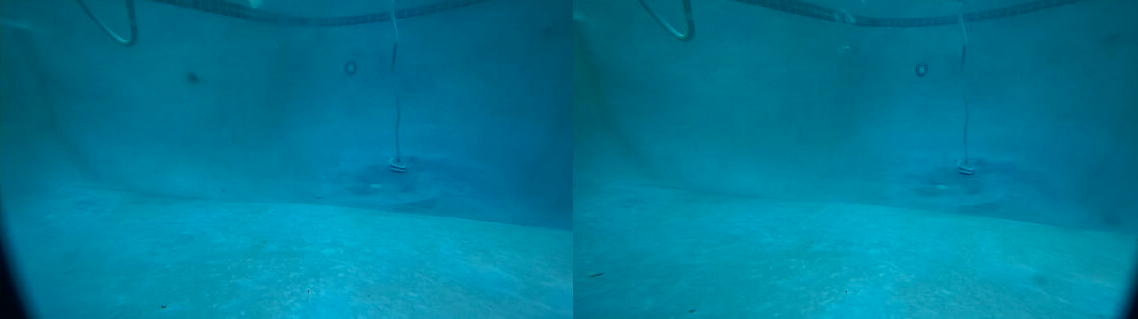
\includegraphics[width=\maxwidth{\textwidth}]{img/zed_pool.png}
\caption{Stereo Camera Output from ZED 2 in uDrone Pool Test}
\legend{\emph{Source}: Photo courtesy of Jnaneshwar Das, used with permission.}
\label{stereo}
\end{figure}

% ***Write the next part after results from JD
% Because light moves differently underwater (expand) the ZED 2 needed to be recalibrated to work underwater. ***DO more here in the future***
% Orientation?
% First go is front facing
% Do we need to do some tests with downward-facing?

\subsection{Blue Robotics Ping Echosounder}
% https://bluerobotics.com/store/sensors-sonars-cameras/sonar/ping-sonar-r2-rp/

The Blue Robotics Ping is a single beam echosounder for measuring distance underwater on the uDrone. It is attached in a downward facing orientation, allowing it to tell the distance of the uDrone to the reef. By aligning it in the same direction as the hyper-spectral sensor it is possible to know the distance to the reef at every moment of sensing. The Ping Echosounder has a range of 0.5 m to 30 m and a beam width of 30 degrees. This device connects to the on board compute via a serial connection and communicates over a ROS node that was developed using the Blue Robotics open-source interface \parencite{pinger}. 

\subsection{Blue Roboitcs Enclosure}
% https://bluerobotics.com/store/watertight-enclosures/8-series/wte8-asm-r1/
The main body of the uDrone needed to be a watertight enclosure to keep the electronic components dry. It also needed to have pass-throughs to communicate with the thrusters and external sensors. A blue robotics enclosure was used to accommodate all of this and reduce the need for precision machining within the lab. Standardizing on the blue robotics system allowed for the rapid prototyping of the uDrone. The 8 inch enclosure was used as it would accommodate all of the electronics inside that were required \parencite{enclosure}.

\subsection{Battery}
The Blue Robotics Lithium-ion Battery was chosen to minimize different suppliers. This 14.8 Volt, 18 Amp-hour battery comes in a cylindrical shape \parencite{batt}. Two of them can fit inside the enclosure with room to spare for other components. With two batteries, one battery will be dedicated to powering the thrusters while the other powers the compute and sensing equipment. The power consumption this latter group is listed in this section are shown in table \ref{power_table}. The total power for internal components is 0.82A at 14V. Adding a 50\% safety factor for calculating run time, the equipment should pull 1.23A, which, with an 18Ah batter will allow for 14.6 hours of run time. A detailed discussion of the power consumption of the thrusters is discussed in section \ref{control_inputs}. From those calculations the thruster run time was determined to be 6 hours, which is more of a limiting factor than the internal equipment.

\begin{table}[h] % Table float
\caption{Power usage of uDrone Internal components}
\label{power_table}
\begin{tabu}{l c} \\ \hline
Component & Power Usage at 14V \\ \hline
Tx2 & 0.54A \\
PixHawk & 0.11A\\
ZED 2 & 0.14A\\
Ping & 0.04A\\\hline
Total & 0.82A\\\hline
\end{tabu}
\legend{\emph{Sources}: \textcite{tx2}, \textcite{px4_pixhawk}, \textcite{zed}, \textcite{t200}}
\end{table}

\begin{figure}[ht]
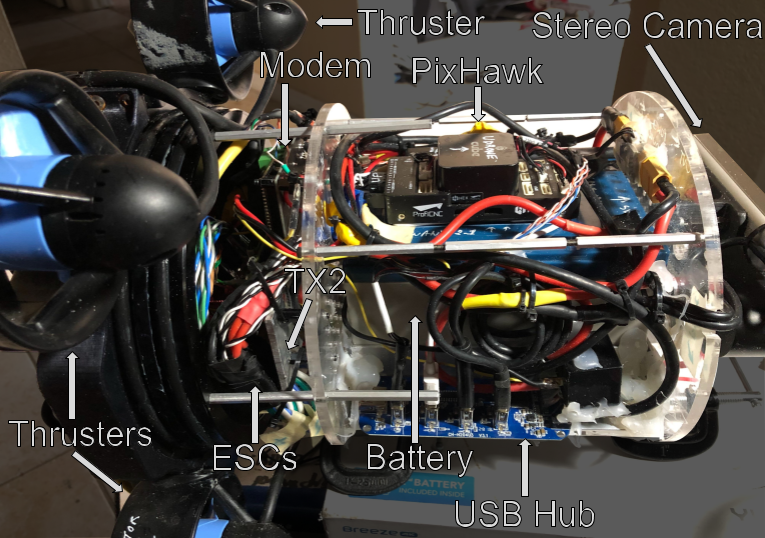
\includegraphics[width=\maxwidth{\textwidth}]{img/side_annotated.png}
\caption{Annotated Picture of uDrone without Enclosure}
\legend{\emph{Source}: Photo courtesy of Jnaneshwar Das, used with permission.}
\label{annotated}
\end{figure}

\section{Software}
In order to function as a testbed for innovation, the uDrone needed to be built using open source and easily accessible software. Additionally, it was desired to use the tools that the DREAMS lab had existing experience with.

\subsection{ROS}
All on board computers run Ubuntu Linux and the Robot Operating System (ROS). ROS is an open source library of tools that are commonly used for robotic systems. The architecture of ROS is similar to a network, consisting of nodes, processes that perform computation, and messages that communicate between notes \parencite{ros,ros-wiki}. All of the sensors, such as the ZED 2 and Ping Echosounder, have existing packages that can communicate with ROS. The sensor data is accessed via a node which generates messages that are used by other nodes. ROS has many additional libraries that are useful for autonomy and other uDrone needs.
% https://www.ros.org/
% http://wiki.ros.org/

\subsection{PX4}
The on board PixHawk flight controller runs PX4 on a nuttX operating system. PX4 is an open source autopilot for drones and other vehicles. This software is used and maintained by a series of academics and other drone developers. There is already a strong knowledge of PX4 from Dr. Das and other members of the DREAMS lab. At its most basic level, PX4 translates desired control inputs, i.e. go to a certain point or rotate clockwise, into specific motor actuation. It uses internal PID controllers to reach set points and mixer files to relate control inputs uniquely for different vehicles. Existing vehicle templates can be used to speed up development of a controller for the uDrone. Specifically, the HippoCampus micro AUV has a similar thruster configuration to the uDrone and was used as a starting point for development \parencite{px4}. 
% https://px4.io/

\subsection{MAVLink and MAVROS}
PX4 communicates using a protocol called MAVLink. There is a ROS package called MAVROS which allows for the translation between ROS messages and MAVLink messages. This package allows for users to write programs with ROS and communicate them directly to the flight controller without needing to write interpreters. This architecture was implemented for the uDrone to allow for fast and seamless development \parencite{mavros}.
% http://wiki.ros.org/mavros

\subsection{QGround Control}
In order to interact with the vehicle while it is running, a ground control software is used. For this project QGround Control is used. This software communicates with the flight controller running PX4 using MAVLink and can be used in both simulation and field trials. It can be used to test manual control, set various types of mission vehicles, and observe the state of the vehicle and all its components. In autonomous mode the vehicle is controlled directly from the on board ROS computer, but QGround Control allows for a window into its operation and provides control overrides when necessary \parencite{qgc}. 

\section{Simulation}
A core component of the whole system is the simulation environment. This allows for testing perception and control methodologies and forms the foundation of all the work that is eventually used on the uDrone. The goal of the simulation environment is to be as close to real life. A diagram showing how all the components of the simulation environment fit together can be seen in figure \ref{soft}. 

This particular setup is used because of its close resemblance to real world deployment. In simulation the control code, which runs with ROS on a desktop or OpenUAV container. In real world deployment this is all run on the internal CPU/GPU on-board the uDrone. The PX4 based flight controller is simulated using SITL while it is run on the PixHawk in deployment. And the simulated world in Gazebo is made to mimic the underwater world and vehicle dynamics that will be experienced in deployment. 

\begin{figure}
    \centering
    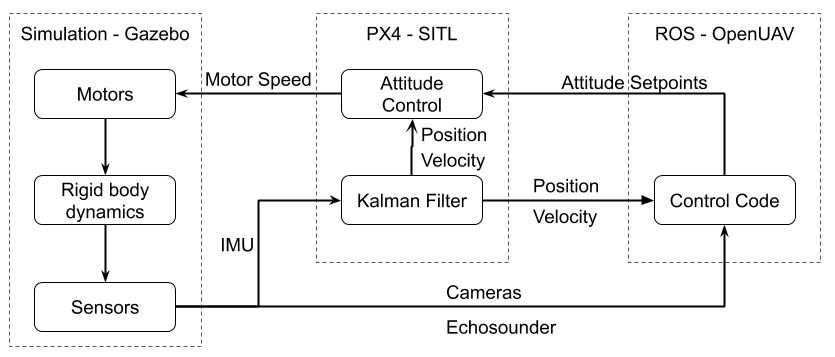
\includegraphics[width=\maxwidth{\textwidth}]{img/soft-sys.png}
    \caption{System diagram showing the interaction between the software components in simulation}
    \label{soft}
\end{figure}

\subsection{Gazebo}
A core component of the entire system is the simulation framework used for development and testing. The simulation of the uDrone is done using Gazebo. Gazebo is a simulator for robotics allowing for the testing of systems in real world like physical environments. It integrates directly with ROS, making development easier. Gazebo allows for the creation of custom worlds and robots, allowing for simulations of the uDrone on a coral reef. PX4 also has a library to work directly with Gazebo, which includes 3D and physics models for many of its vehicle templates. For most development, ROS is run and PX4 is emulated on the host system. Using this setup it is also possible to run hardware-in-the-loop simulations, allowing for tests of the performance of the TX2 and PixHawk Cube \parencite{gazebo}. 
% http://gazebosim.org/

\subsection{UUV Simulator}
To make the Gazebo environment as real as possible, a package called the Unmanned Underwater Vehicle Simulator (UUV Sim) was used to simulate the effects of a vehicle moving underwater. UUV Sim was specifically designed to aid in the simulation of underwater vehicles. This packages main contribution and reason it was used on this project is the implementation of the equations of motion detailed by Thor Forsson in the Handbook of Marine Hydrodynamics. It also has improved thruster models, several controllers purpose built for AUVs, aquatic world files, and several vehicle models \parencite{uuv}. 
% https://uuvsimulator.github.io/

% \subsection{Unity}
% While Gazebo is a very useful simulator for physics, other simulators are available for better photo-realism. As part of the uDrone project the Unity game engine was used in conjunction with Gazebo for better photorealism. In this setup, the two simulator environments act in a master-slave fashion. The vehicle position, orientation, and movement is controlled in Gazebo. This data is then sent to Unity, which moves the vehicle accordingly. The cameras are modeled in Unity and they send back data to ROS based on what they see in this simulation. Controllers in ROS then use this data to send control signals through PX4 back to Gazebo. For more information on this setup and its application, see Harish’s Thesis.

\subsection{Reef Data}

One of the main challenges to creating a simulation environment to test the uDrone was in finding a model of a reef to test with. To obtain a realistic reef model I took video footage while recreational scuba diving in Kona, Hawaii. This was a particularly good spot since the dives sites were only a few miles away from the planned initial site of the uDrone deployment. I built a special rig that allowed me to hold two GoPro cameras while I dove. The goal of the two cameras was to get a wider spread and possibly use them together as a stereo pair. Because the cameras were not synced, the stereo pair plan did not work.

The 3D model was generated from the footage using Agisoft Metashape structure from motion software. The videos, originally shot at 30 frames per second, needed to be down sampled to 6 frames per second. This allowed for some overlap between each image but not so much that processing took too long. Next, Agisoft found feature correspondence between the overlapping images. With this information, the software was able to generate a mesh and full 3D model with a photographic overlay, seen in figure \ref{reef}. 

\begin{figure}[h]
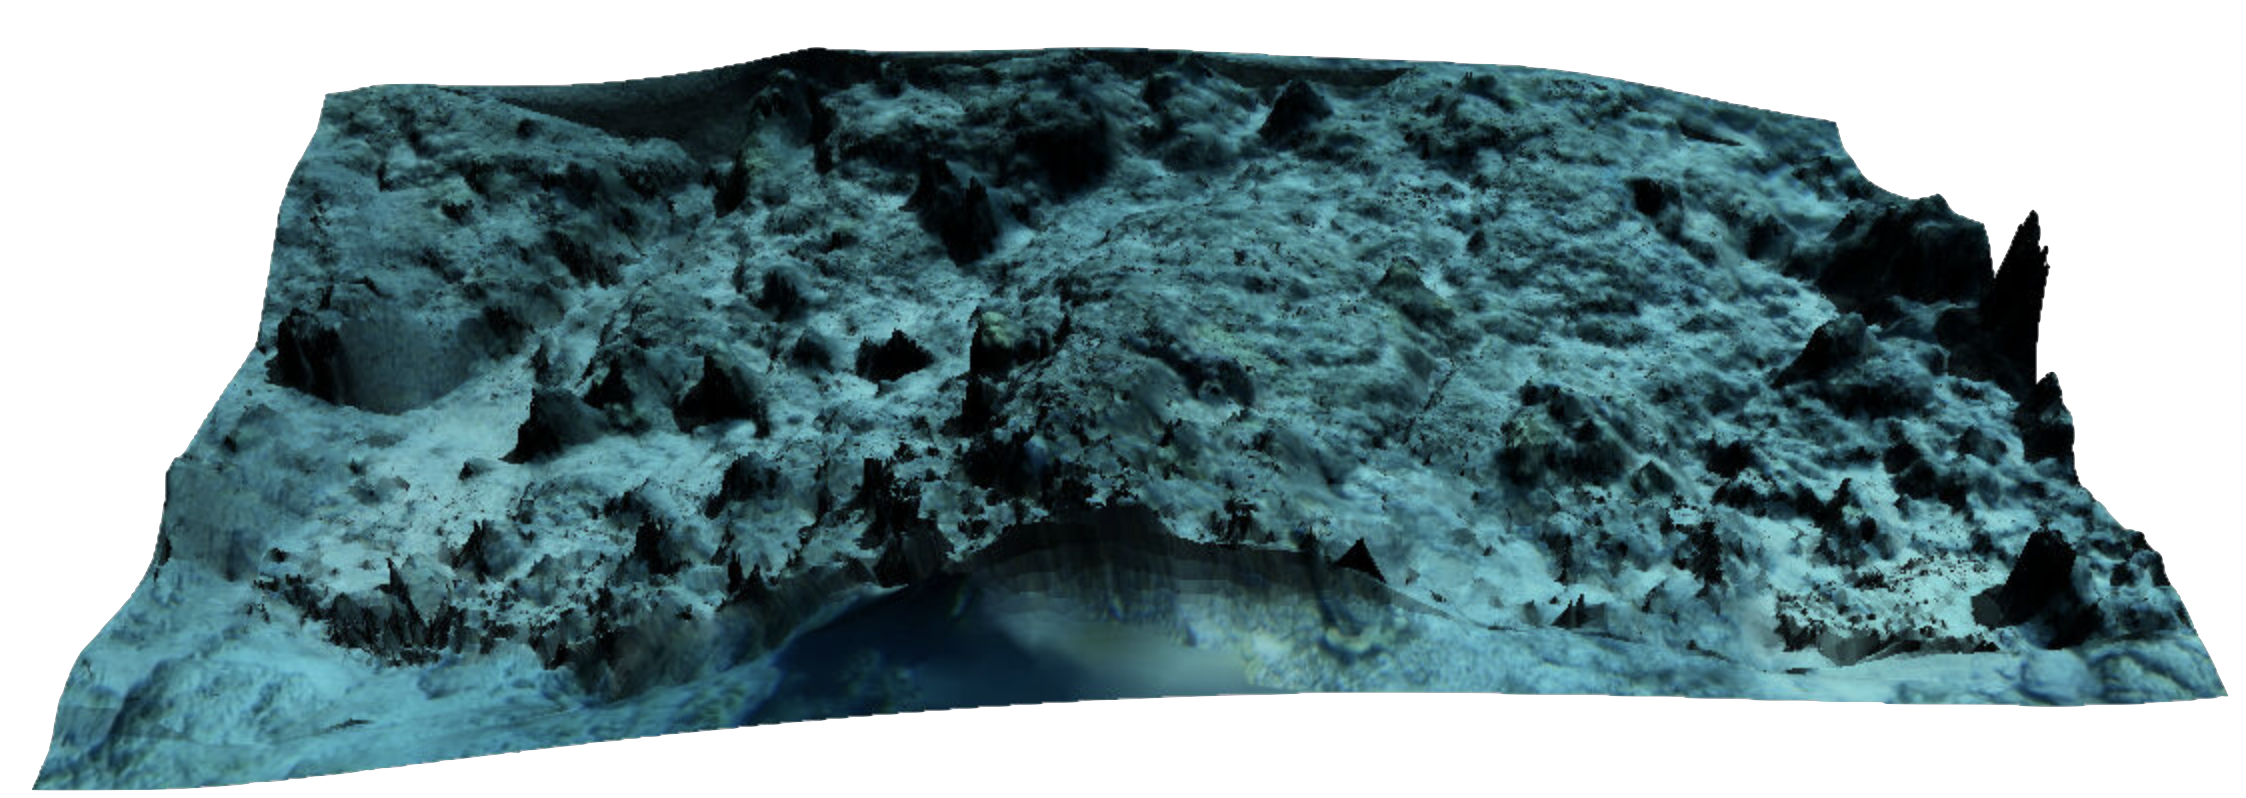
\includegraphics[width=\maxwidth{\textwidth}]{img/reef.png}
\caption{Three Dimensional Reef Model for Simulation}
\label{reef}
\end{figure}

This process was not without significant challenges. Since there are many suspended particles in the water, structure from motion would often mistake these for features and incorporate them into the surface. For this reason, although many videos were shot, only one was able to be turned into a reliable reef model. The 3D model came from a section of the Kaloko Arches dive site near Kona, Hawaii. While the exact dimensions cannot be determined using this method, the model is estimated to be 16 by 8 meters.

% This model served its purpose for early works and proof of concept. Later in the project we received much larger and higher fidelity reef models from Dr. John Burns at University of Hawaii in Hilo. As part of his reef monitoring and conservation studies, he and his team conduct thorough imaging surveys of sections of the reef and convert them into 3D models. These models are incorporated into the Unity simulation framework that is used for greater photorealism. 

% https://www.johnhrburns.com/


\section{Construction}
% The physical design and construction of the vehicle was led by an expert modeler and builder, Cole Brower. He was aided by an undergraduate, Rodney Staggers, Jr., working on a NASA Space Grant (***CHECK THIS***). First, rough drawings were generated by the stakeholders on the project. Using these sketches, the build team created a full 3D model of the vehicle, including all internal & external components. 

The internal frame that supported the batteries and other electrical equipment and the external coupling for the thrusters were 3D printed based on designs. The whole vehicle was then assembled and prepared for testing. By leveraging 3D printing the team was able to test our and rapidly prototype design ideas. Also, since the structural components are easier to source as they can be 3D printed almost anywhere. 

One major change that came about during this construction process involved the design of the interior structure. This structure went through several iterations in order to make physically working on the uDrone easier. Specifically, the compute cluster was repositioned so it would be closer to the camera in the front and easier to access without removing the batteries. Additionally, the entire structure was built to be removed as one solid piece, allowing for easy access when inserting into the enclosure. 


% \begin{itemize}
%     \item Constant Speed
%     \item Constant Distance to Reef
%     \item Carry Scientific Equipment
%     \item Easy to Deploy
% \end{itemize}

% \section{Design Motivation}
% \subsection{Background}
% Underwater vehicles and Underwater Propulsion methods
% \subsection{Quadcopters}
% Mimic design and control
% Leverage Drone infrastructure

% \section{Actuation}
% \subsection{Enclosure}
% \subsection{Thrusters}

% \section{Perception}
% \subsection{Acoustic Pinger}
% \subsection{ZED Stereo Camera}
% \subsection{Other Sensors}

% \section{Automation}
% \subsection{Background}
% \subsection{Pixhawk/Px4}
% \subsection{Tx2}
% \subsection{ROS}

                     %   \include rather than \input for chapters
\chapter{Mathematical Model of Vehicle Dynamics}

This chapter will detail the mathematical model that was developed to describe the motion of the uDrone. 

\section{Reference Frames and State Space}

Conventions for creating this model will follow those laid out by Thor Fossen in the 2011 Handbook of Marine Craft Hydrodynamics and Control. The fixed world frame is defined using the North-East-Down (NED) coordinate system, represented as $\{n\} = (x_n, y_n, z_n)$. in this system, $x_n$ points North, $y_n$ points East, and $z_n$ points down. 

The body-fixed frame $\{b\} = (x_b, y_b, z_b)$ is fixed its origin point, $o_b$, to the uDrone. For purposes of this model, $o_b$ is set at the point on the plane of the motors at the back of the uDrone that is along its center-line. $x_b$ runs along the center-line of the vehicle, pointing from the aft (back) of the uDrone to the fore (front). $z_b$ runs from top to bottom and, following the right-hand rule, $y_b$ runs towards the starboard (right). Further, following convention, roll is defined as rotation about $x_b$, pitch as rotation about $y_b$, and yaw as rotation about $z_b$, with counter-clockwise (CCW) being the positive direction. 

This choice of body frame origin reduces the complexity of modeling the forces produced by the motors. The drawback is some added complexity caused by the moments of the center of buoyancy and center of gravity relative to the chosen origin, but this is more straight forward than the complexity of calculating motor forces about a different point.

The position of the vehicle, or the body-fixed frame $\{b\}$, with respect to the world frame $\{n\}$ is expressed as $\bm{p} = [N, E, D]^T$. The attitude of the vehicle is expressed as $\bm{\Theta} = [\phi, \theta, \psi]^T$ using Euler angles. Together these create the 6-dimensional position/orientation vector $\bm{\eta} = [\bm{p}, \bm{\Theta]}^T$. The linear and angular velocities are expressed with respect to the vehicles fixed frame $\{b\}$. The linear velocity is $\bm{v} = [u, v, w]^T$ and angular velocity $\bm{\omega} = [p, q, r]^T$. when combine, these form the combine 6-dimensional velocity vector $\bm{\nu}= [\bm{v}, \bm{\omega]}^T$. All together, $\boldsymbol{\eta}$ and $\boldsymbol{\nu}$ represent the 12-dimensional state space describing the state of the uDrone \parencite{thor_kin}. 

% \begin{align*}
%      \boldsymbol{p}^{n}_{b}=\left[\begin{array}{c}
%         N \\ E \\ D
%      \end{array}\right]
%      \bm{\Theta}^{n}_{b}=\left[\begin{array}{c}
%         \phi \\ \theta \\ \psi
%      \end{array}\right]
%      \bm{\eta}=\left[\begin{array}{c}
%         \bm{p} \\ \bm{\Theta}
%      \end{array}\right]
% \end{align*}
% \begin{align*}
%      \boldsymbol{v}^{b}_{b}=\left[\begin{array}{c}
%         u \\ v \\ w
%      \end{array}\right]
%      \bm{\omega}^{b}_{b}=\left[\begin{array}{c}
%         p \\ q \\ r
%      \end{array}\right]
%      \bm{\nu}=\left[\begin{array}{c}
%         \bm{v} \\ \bm{\omega}
%      \end{array}\right]
% \end{align*}



\section{Equations of Motions}

The general equation of motion for the uDrone can be derived as a function of the combine linear and angular velocity vector $\boldsymbol{\nu}$ \parencite{thor_mod}. This is shown in equation \ref{eqm}.

\begin{gather}
\underbrace{\boldsymbol{M}_{R B} \dot{\boldsymbol{\nu}}+\boldsymbol{C}_{R B}(\boldsymbol{\nu}) \boldsymbol{\nu}}_{\text {rigid-body forces}}+\underbrace{\boldsymbol{M}_{A} \dot{\boldsymbol{\nu}}+\boldsymbol{C}_{A}\left(\boldsymbol{\nu}\right) \boldsymbol{\nu}+\boldsymbol{D}\left(\boldsymbol{\nu}\right) \boldsymbol{\nu}}_{\text {hydrodynamic forces}}+\underbrace{\boldsymbol{g}(\boldsymbol{\eta})}_{\text{hydrostatic forces}}=\boldsymbol{\tau}
\label{eqm}
\end{gather}
With the terms defined as:
\begin{align*}
    \boldsymbol{\eta}&=\text{combine position and orientation}\\
    \boldsymbol{\nu}&=\text{combine linear and angular velocity}\\
    \dot{\boldsymbol{\nu}}&=\text{combine linear and angular acceleration}\\
    \boldsymbol{M}_{R B}&=\text{rigid-body system inertia matrix}\\
    \boldsymbol{C}_{R B}(\boldsymbol{\nu})&=\text{rigid-body Coriolis matrix}\\
    \boldsymbol{M}_{A}&=\text{added mass system inertia matrix}\\
    \boldsymbol{C}_{A}(\boldsymbol{\nu})&=\text{added mass Coriolis matrix}\\
    \boldsymbol{D}(\boldsymbol{\nu})&=\text{damping matrix}\\
    \boldsymbol{g}(\boldsymbol{\eta})&=\text{gravitational and buoyant forces}\\
    \boldsymbol{\tau}&=\text{control inputs}
\end{align*}
% \begin{align*}
%     \boldsymbol{\eta}&=\text{combine position and orientation}\\
%     \boldsymbol{\nu}&=\text{combine linear and angular velocity}\\
%     \dot{\boldsymbol{\nu}}&=\text{combine linear and angular acceleration}\\
%     \boldsymbol{\tau}&=\text{control inputs}\\
%     \boldsymbol{M}&=\text{system inertia matrix}\\
%     \boldsymbol{C}(\boldsymbol{\nu})&=\text{Coriolis matrix}\\
%     \boldsymbol{D}(\boldsymbol{\nu})&=\text{damping matrix}\\
%     \boldsymbol{g}(\boldsymbol{\eta})&=\text{gravitational and buoyant forces}\\
%     \boldsymbol{\tau}&=\text{control inputs}
% \end{align*}
% \begin{align*}
%     \boldsymbol{M}&=\boldsymbol{M}_{R B}+\boldsymbol{M}_{A}\\
%     \boldsymbol{C}&=\boldsymbol{C}_{R B}+\boldsymbol{C}_{A}
% \end{align*}

\section{Rigid-Body Forces}

The exact values of the system inertia ($\boldsymbol{M}$), Coriolis ($\boldsymbol{C}$), and Drag ($\boldsymbol{D}$) matrices can be determined either through intensive hydrodynamic modeling or experimentation. Due to the complexity of hydrodynamic modeling, experimentation is typically used to determine these values in underwater vehicles similar to the uDrone \parencite{hipp_pen}. It is possible, however, to estimate the rigid body matrix values using information about the vehicle generated from the 3D model. This section details these estimations and explains how they were calculated. 

The rigid body system inertia matrix about the center of origin can be calculated using equation \ref{mrb} which is found in \cite{thor_rb}.
\begin{gather}
    \boldsymbol{M}_{R B}^{C O}=\left[\begin{array}{cc}
        m \boldsymbol{I}_{3 \times 3} & -m \boldsymbol{S}\left(\boldsymbol{r}_{g}^{b}\right) \\
        m \boldsymbol{S}\left(\boldsymbol{r}_{g}^{b}\right) & \boldsymbol{I}_{g}-m \boldsymbol{S}^{2}\left(\boldsymbol{r}_{g}^{b}\right)
    \end{array}\right]
    \label{mrb}
\end{gather}
% \begin{align*}
%     \boldsymbol{M}_{R B}^{C O}&=\text{rigid body system inertia matrix about the body fixed-frame origin}\\
%     \boldsymbol{I}_{3 \times 3}&=\text{3 by 3 identity matrix}\\
%     m&=\text{mass}\\
%     \boldsymbol{S}(\cdot)&=\text{cross product operator}\\
%     \boldsymbol{r}_{g}^{b}&=\text{ vector from the body fixed-frame origin to the center of gravity}\\
%     \boldsymbol{I}_{g}&=\text{inertia matrix}
% \end{align*}

In this equation, $m$ is the mass, $\boldsymbol{I}_{3 \times 3}$ is the three-by-three identity matrix, $\boldsymbol{I}_{g}$ is the inertia matrix and $\boldsymbol{r}_{g}^{b}$ is the vector from the body fixed-frame origin to the center of gravity. $\boldsymbol{S}$ is the cross product operator matrix. Before the final vehicle was constructed, m, $\boldsymbol{I}_{g}$, and $\boldsymbol{r}_{g}^{b}$ were taken from the 3D model. Those estimates are shown in equation \ref{m_matrix}.

\begin{equation}
\boldsymbol{M}_{R B}^{C O}=\left[\begin{array}{cccccc}
9.9000 & 0 & 0 & 0 & 0 & 0 \\
0 & 9.9000 & 0 & 0 & 0 & 1.4850 \\
0 & 0 & 9.9000 & 0 & -1.4850 & 0 \\
0 & 0 & 0 & 0.3420 & 0.0010 & -0.0001 \\
0 & 0 & -1.4850 & 0.0010 & 0.5577 & -0.0015 \\
0 & 1.4850 & 0 & -0.0001 & -0.0015 & 0.3167
\end{array}\right]
\label{m_matrix}
\end{equation}


With a completed vehicle these numbers can be verified and varied if needed. For example, with no ballast, the uDrone is positively buoyant. Therefore, to maintain its depth without using power to stay underwater ballast will need to be added. By placing the ballast closer to the center of the vehicle, the moments of inertia will decrease. Conversely, by placing it further from the center the moments can be increased. Additionally, the ballast can be used to change the center of gravity relative to the center of buoyancy. This will create a moment in the vehicle that can help it stay oriented or level in specific ways. This relationship is discussed further in the section \ref{hydrostatics}. 

The Coriolis matrix is a function of the angular velocity of the vehicle and can be derived as shown in equation \ref{crb} from \cite{thor_rb}.
\begin{gather}
    \boldsymbol{C}_{RB}^{CO}(\boldsymbol{\nu})=\left[\begin{array}{cc}
        m \boldsymbol{S}\left(\boldsymbol{\omega}^{b}\right) & -m \boldsymbol{S}\left(\boldsymbol{\omega}^{b}\right) \boldsymbol{S}\left(\boldsymbol{r}_{g}^{b}\right) \\
        m \boldsymbol{S}\left(\boldsymbol{r}_{g}^{b}\right) \boldsymbol{S}\left(\boldsymbol{\omega}^{b}\right) & -\boldsymbol{S}\left(\left(\boldsymbol{I}_{g}-m \boldsymbol{S}^{2}\left(\boldsymbol{r}_{g}^{b}\right)\right) \boldsymbol{\omega}^{b}\right)
    \end{array}\right]
    \label{crb}
\end{gather}
% \begin{align*}
%     \boldsymbol{C}_{R B}^{C O}&=\text{rigid body Coriolis matrix about the body fixed-frame origin}\\
%     m&=\text{mass}\\
%     \boldsymbol{S}(\cdot)&=\text{cross product operator}\\
%     \boldsymbol{\omega}^b&=\text{body-fixed frame angular velocity}\\
%     \boldsymbol{r}_{g}^{b}&=\text{ vector from the body fixed-frame origin to the center of gravity}\\
%     \boldsymbol{I}_{g}&=\text{inertia matrix}
% \end{align*}

Where $\boldsymbol{\omega}^{b}$ is the body-fixed frame angular velocity vector. Since this matrix is a function of the vehicle state, it will change with motion. The actual calculations of this matrix are handled by a MatLab program written as a companion to Thor Forson’s book \parencite{mss}. The values based on the system inertia matrix in equation \ref{m_matrix} along with a velocity state vector $\bm{\nu}= [1,0,0,0,0,0]^T$, which represents only forward motion, is shown in equation \ref{c_matrix}.

\begin{equation}
\boldsymbol{C}_{RB}^{CO}(\boldsymbol{\nu})=\left[\begin{array}{cccccc}
0 & 0 & 0 & 0 & 0 & 0 \\
0 & 0 & 0 & 0 & 0 & 9.9000 \\
0 & 0 & 0 & 0 & -9.9000 & 0 \\
0 & 0 & 0 & 0 & 0 & 0 \\
0 & 0 & 9.9000 & 0 & 0 & 0 \\
0 & -9.9000 & 0 & 0 & 0 & 0
\end{array}\right]
\label{c_matrix}
\end{equation}

\section{Hydrostatic Forces} \label{hydrostatics}

The hydrostatic term $\boldsymbol{g}(\boldsymbol{\eta})$ accounts for the forces on the uDrone caused by gravity and buoyancy. The force of gravity, or weight ($W$) is equal to the mass of the uDrone times the acceleration due to gravity. The buoyant force ($B$) is the weight of the water displaced by the uDrone. This is calculated by multiplying the volume of the uDrone, the density of water, and the acceleration due to gravity. If the location of the center of gravity and center of buoyancy (or center of volume) of the uDrone are not in the same spot then there will be a moment on the whole vehicle. Similarly, if the two forces are not equal then there will also be a net linear force on it. This value is a function of the orientation of the vehicle and can be seen in equation \ref{bigG} \parencite{thor_rb}. 

\begin{equation}\label{bigG}
\boldsymbol{g}(\boldsymbol{\eta})=\left[\begin{array}{llll} 
& (W-B) \sin (\theta) \\
- & (W-B) \cos (\theta) \sin (\phi) \\
- & (W-B) \cos (\theta) \cos (\phi) \\
- & \left(y_{g} W-y_{b} B\right) \cos (\theta) \cos (\phi) & + & \left(z_{g} W-z_{b} B\right) \cos (\theta) \sin (\phi) \\
& \left(z_{g} W-z_{b} B\right) \sin (\theta) & + & \left(x_{g} W-x_{b} B\right) \cos (\theta) \cos (\phi) \\
- & \left(x_{g} W-x_{b} B\right) \cos (\theta) \sin (\phi) & - & \left(y_{g} W-y_{b} B\right) \sin (\theta)
\end{array}\right]
\end{equation}

% \begin{equation}
%   \boldsymbol{g}(\boldsymbol{\eta})=\left[\begin{array}{llll}  
%   0\\0\\0\\0\\0\\0
%   \end{array}\right]
% \end{equation}

Ballasting can be used to adjust the weight and center of mass on the uDrone. To simplify this equation the ballast is set so that the weight and buoyancy are equal and the center of mass and buoyancy are the same. This means the $\boldsymbol{g}$ vector will be zeros for all $\boldsymbol{\eta}$. These forces can be seen interacting on the uDrone in figure \ref{cord_frame}. Maintaining overlapped centers of buoyancy and gravity also makes the vehicle more nimble as there are less moments to overcome when rotating. This also has the benefit of making the uDrone more maneuverable. Equal weight and buoyancy reduces energy used as the uDrone does not need to overcome a force making it sink or float as it cruises through the water column. 

There might be reasons to adjust the ballasting of the uDrone to impart other properties on it. For example, if the vehicle is slightly positively buoyant than it will float in the event of a power failure, allowing for it to be recovered more easily. Also, if the center of gravity is placed below the center of buoyancy, but still in line with it in the z body direction, then the vehicle will be self righting in roll. This could make control easier as roll, which should be at zero most of the time, can be ignored.

\section{Hydrodynamic Forces} \label{hydrodynamics}

The added mass system inertia matrix and added mass Coriolis matrix can only be determined through experimentation or complex fluid dynamic simulation and are not calculated in the scope of this thesis. The damping matrix, however, can be estimated using drag calculations. 

The vehicle is modeled as a flat-faced cylinder moving through water in a direction along its axis. This estimation neglects two factors: 1) drag from the motors, and 2) rotational damping. Both of these forces are small in comparison to the drag of the flat-faced cylinder, so for the purposes of an approximate model, they can be ignored. 

The force of drag in a single direction can be calculated using the drag equation:

\begin{gather}
F_{D}=C_{D} A \frac{\rho V^{2}}{2}
\end{gather}
\begin{align*}
    F_D&=\text{drag Force}\\
    C_D&=\text{coefficient of drag}\\
    A&=\text{cross-sectional area normal to velocity}\\
    \rho&=\text{fluid density}\\
    V&=\text{velocity}\\
\end{align*}

Based on the ratio of the diameter to the length of the main body of the uDrone, the Coefficient of drag in the direction of motion is estimated at 0.8. The density of salt water is 1024kg/m$^3$ and the surface area is calculated from the diameter of the eight inch cylinder, which is 0.037m$^2$. Putting this all together, damping force can be calculated as a function of velocity. This is:

\begin{gather}
    \boldsymbol{D}(\boldsymbol{\nu})\boldsymbol{\nu}=\left[\begin{array}{c}
        -15.0u ^2 \\ \sim 0 \\ \sim 0 \\ D_{roll} \\ D_{pitch} \\ D_{yaw}
     \end{array}\right]
\end{gather}

$u$ is the velocity in the x body direction. The last three values which refer to the rotational damping. For the purposes of calculations in the next section these values were assumed to be zero. The second and third terms, however, will always be zero, or nearly zero, as the vehicle cannot independently move in the Y or Z direction.

\section{Control Inputs}\label{control_inputs}

The control inputs are the forces put on the uDrone from the thrusters. The four motor of the uDrone are arranged on a plane, all facing the same direction. The center point between all the thrusters along that plane is the Center of Origin $C_O$ for the vehicle. Thrusters one and three spin in a counterclockwise direction while thrusters two and four spin clockwise for forward thrust. This ensures that the vehicle has no roll moment when moving forward. Figure \ref{cord_frame} shows the uDrone with the $C_O$ and rotation direction of the thrusters. 

\begin{figure}[h]
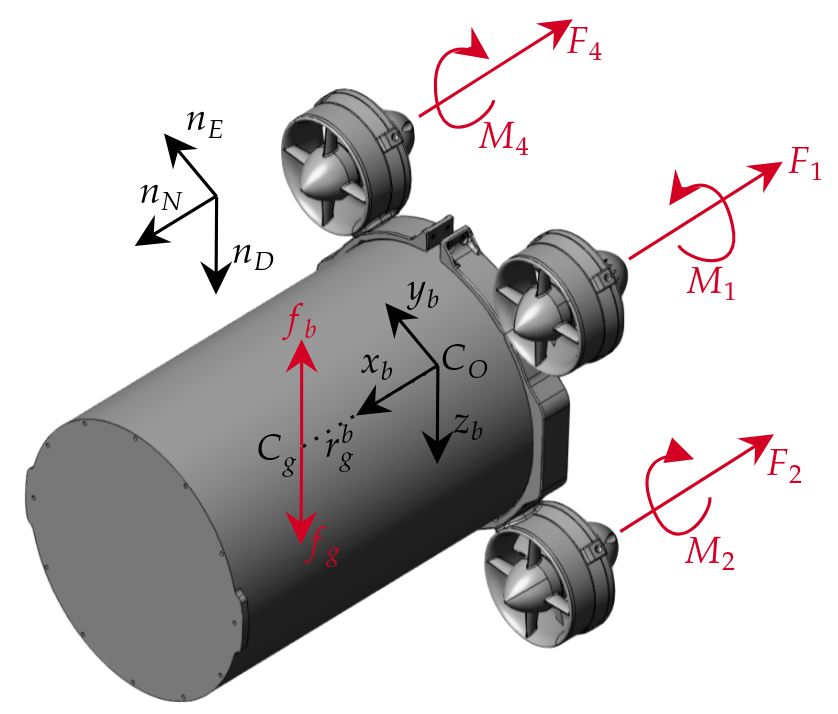
\includegraphics[width=\maxwidth{\textwidth}]{img/cord_frame.png}
\caption{uDrone Coordinate Frame and Motor Directions}
\label{cord_frame}
\end{figure}

Using this convention it is possible to determine the actuation matrix, tau, as a function of thruster inputs.

\begin{gather}
    \boldsymbol{\tau}=\left[\begin{array}{c}
        F_1+F_2+F_3+F_4 \\ 0 \\ 0 \\ M_1-M_2+M_3-M_4 \\ (F_2+F_3-F_1-F_4) \frac{L}{\sqrt{2}} \\ (F_1+F_2-F_3-F_4) \frac{L}{\sqrt{2}}
     \end{array}\right]
     \label{tau}
\end{gather}

In equation \ref{tau} $F_x$ indicates the linear force produced by the $x^{th}$ motor and $M_x$ indicates the angular momentum produced by the $x^{th}$. $L$ is 0.115m, the length from $C_O$ to the center of the motor, which is the same for each motor. Unfortunately, there is no data from Blue Robotics about the moment of the thrusters, so the relationship between control input to the roll moment will need to be determined experimentally. Data is available, however, correlating motor power and thrust force. 

\begin{figure}[h]
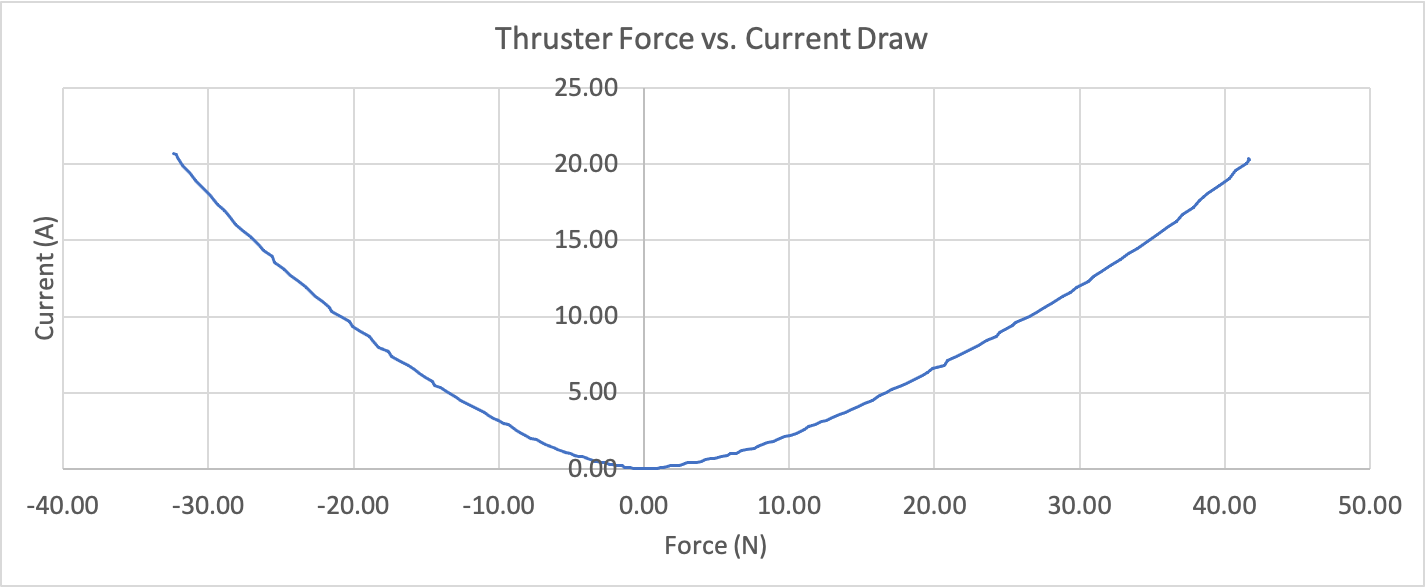
\includegraphics[width=\maxwidth{\textwidth}]{img/force_amps.png}
\caption{Force Output vs. Current Draw for T200 Thruster at 14 Volts}
\label{force_amp}
\legend{\emph{Source}: \iftoggle{usebiblatex}{\textcite{t200}}{\citet{t200}}}% See: https://upload.wikimedia.org/wikipedia/commons/8/89/Antidorcas_marsupialis%2C_male_%28Etosha%2C_2012%29.jpg
% \legend{\emph{Note}: Here is a note that is especially long to show what happens when it extends to more than one line.}
\end{figure}


Using the figure \ref{force_amp}, along with data about the uDrone battery, it is possible to calculate the maximum velocity, running time at this velocity, and running time at the operational velocity of 1m/s. While the uDrone can carry two 14V, 18Ah batteries, the intent is to use one for thrusters and the other to control all electronics. Therefore, all longevity calculations are done assuming 18Ah are available for thruster actuation. 

In order to calculate maximum velocity, the drag equation is set equal to the maximum thruster force. The T200 thrusters produce a maximum thrust of 41.68N each. This is 166.7N of total thrust. Setting this equal to $15u^2$ and solving yields a maximum speed of 3.33m/s. Maintaining this velocity takes 20.29A, for a total of 81.16A. The uDrone could only maintain this speed for approximately 13.3 minute with an 18Ah battery.

Typically, however, the uDrone will be cruising at a speed of 1m/s. At this speed, the drag force is approximately 15N. To maintain this thrust each motor must produce about 3.75N of force. To maintain this force each motor will use approximately 0.5A, for a total of 2A. In order to stay conservative, a 50\% safety factor will be added to this value to account for uncalculated drag forces and actuation that affect orientations, not just forward motion. With this addition, the vehicle will use 3A for actuation during normal operation. With a single 18Ah battery used for thrusters, this will yield a dive time of approximately 6 hours. 
% etc.
\chapter{Optimal Control in Two-Dimensional Space}\label{2d}

In this project \footnote{This particular application was completed as part of a group project undertaken by the author along with Evan Lamb and Jason Newton. Parts of this section are re-purposed from the project report.}, the principles of optimal control were applied to the uDrone. In order to simplify the process, the vehicle and world were modeled as a two-dimensional system with one control input. Dynamic programming was used with a cost function that satisfies the mapping goals of the vehicle while minimizing control input. This section lays out the methods, implementation, and results of this particular application.

\section{Methods}
\subsection{Simplification \& Assumptions}
In order to reduce the complexity of this problem, the vehicle and world are modeled in two dimensions. Since the goal of the vehicle is to move in a straight line along the reef in the X-Z plane (where Z is down and X is forward), this is a reasonable assumptions. To further simplify the problem, the forward thrust is assumed to be at a constant value and the only control input is pitch rate. More assumptions were made to simplify the dynamic model, including constant forward drag, no rotational drag, no Coriolis forces, neutral buoyancy, corresponding centers of buoyancy and mass, and discrete state transitions. 

\subsection{Model}
The first step of this project involved generating a model for the uDrone, defining a cost function, and determining constraints. 

% \begin{figure}[t]
%     \centerline{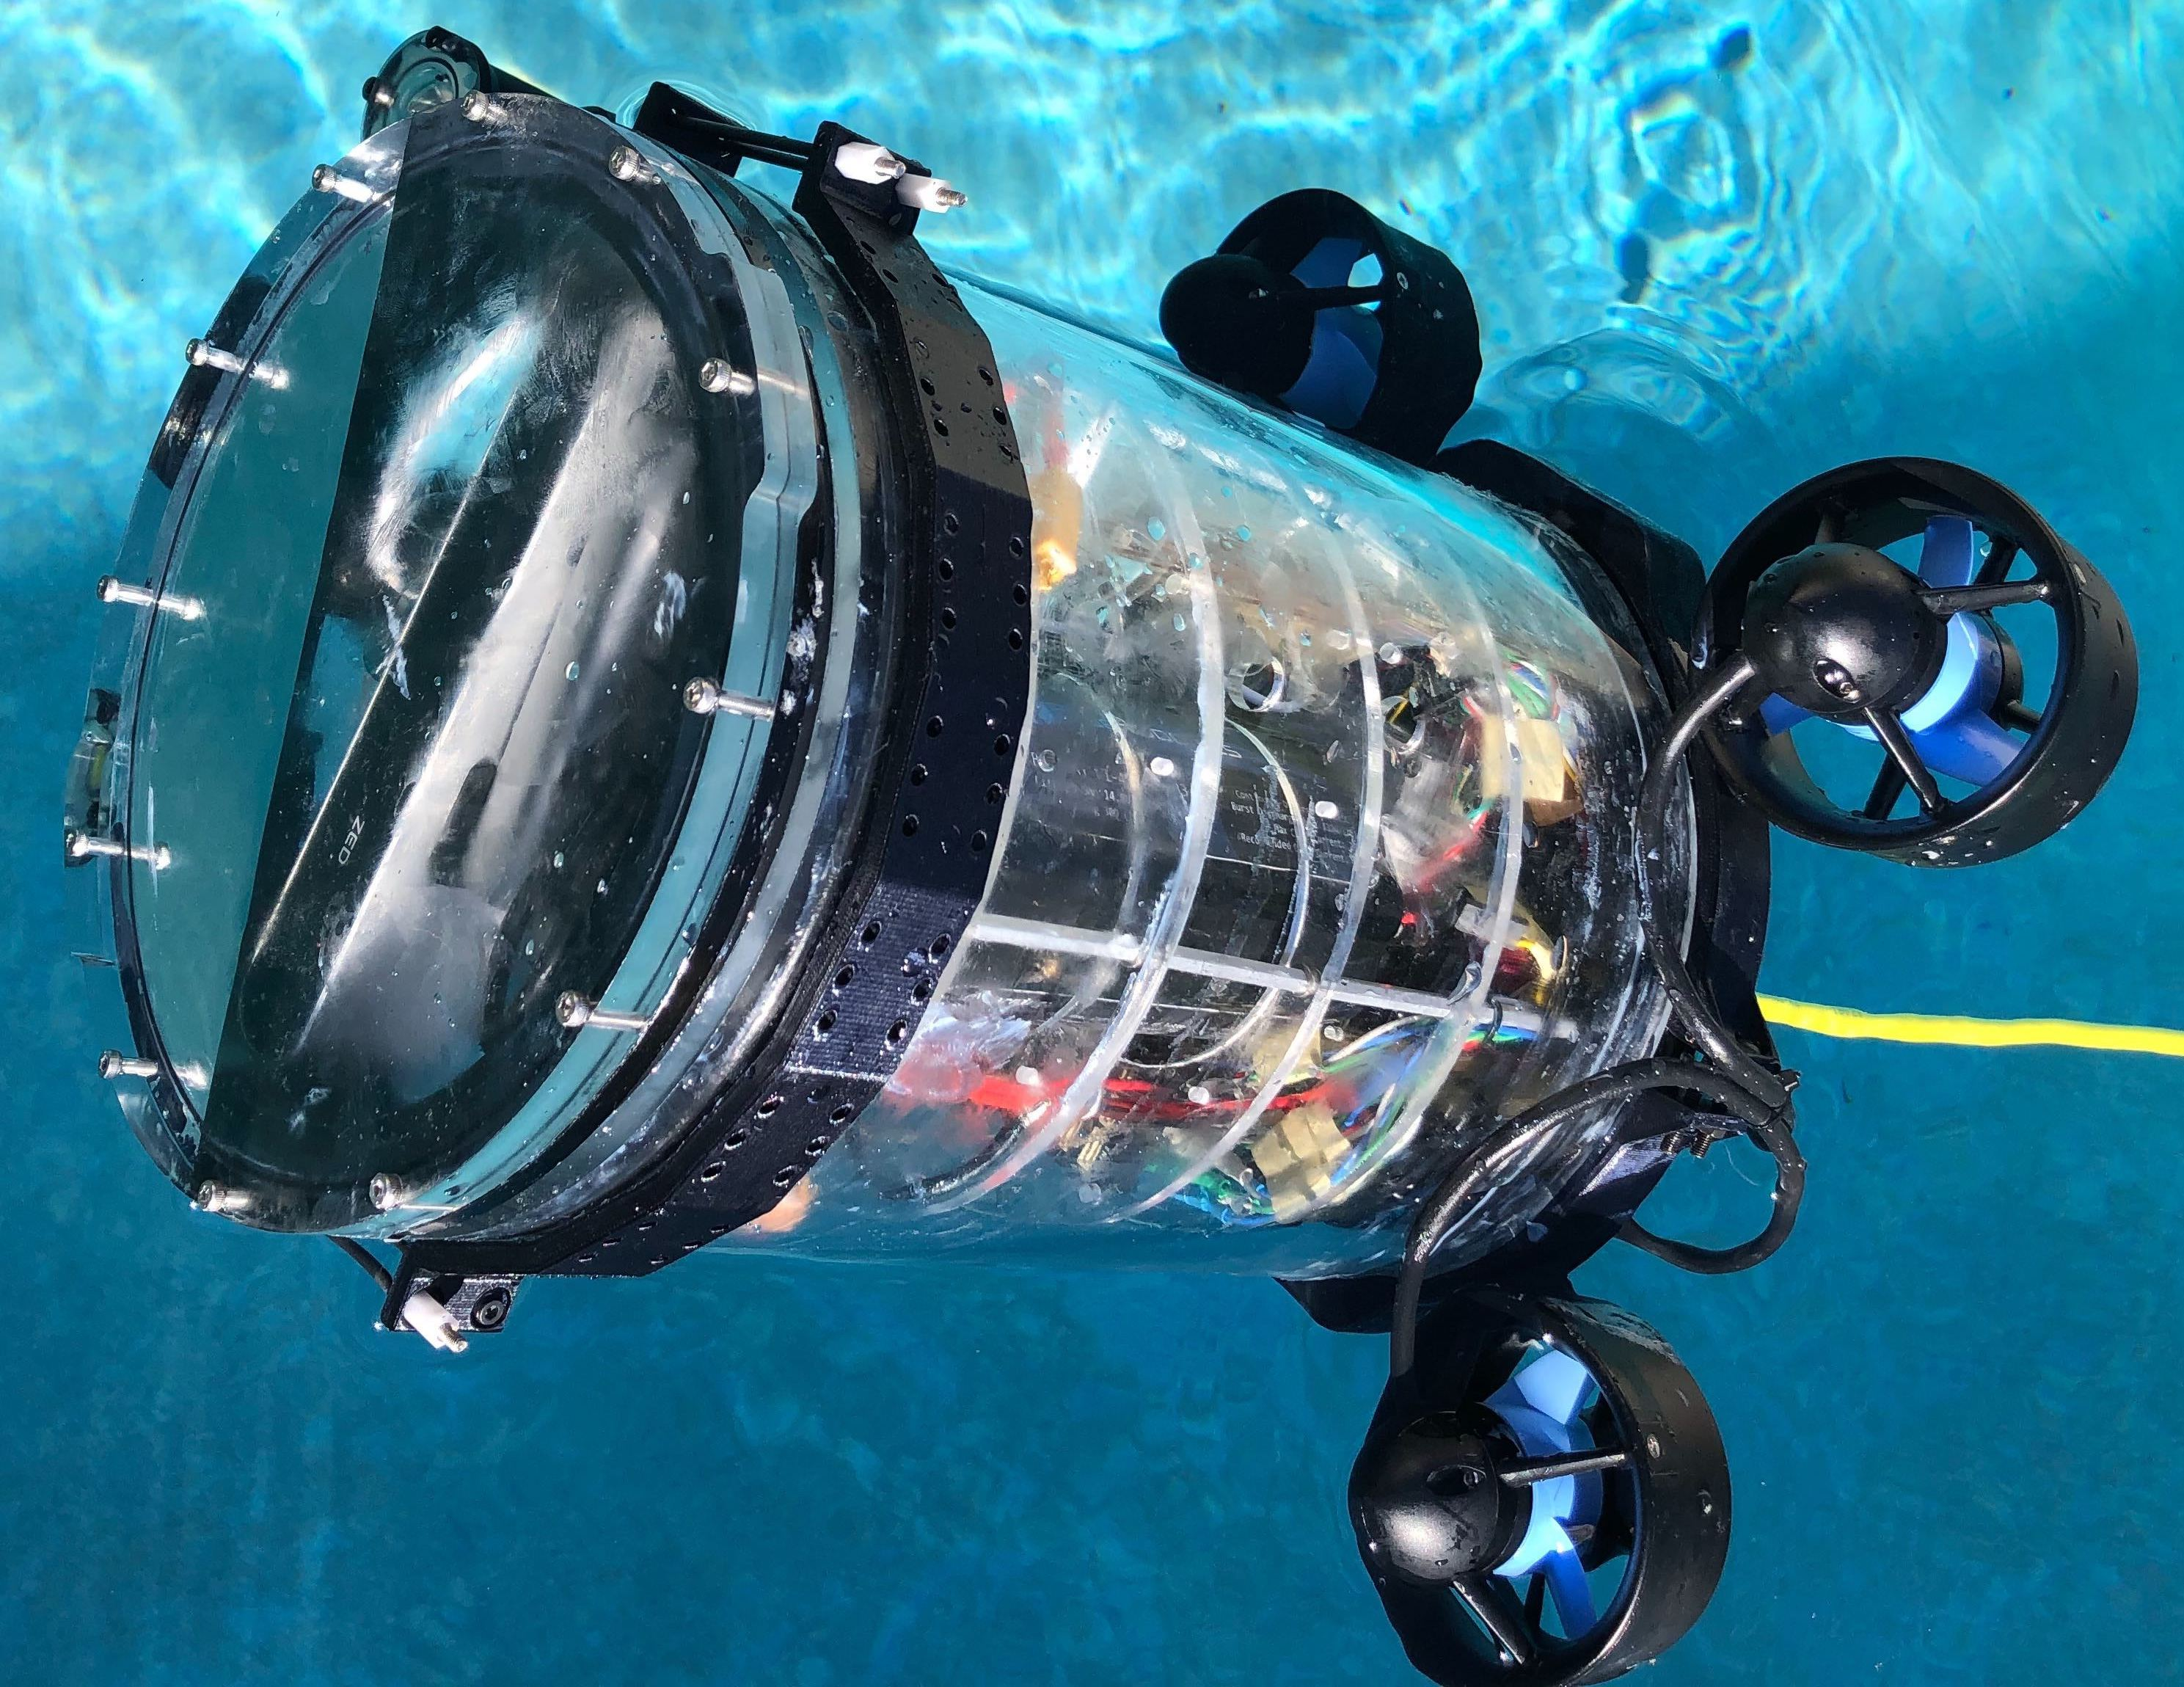
\includegraphics[width=\linewidth]{img/drone_pool.jpg}}
%     \caption{The uDrone}
%     \label{fig:drone}
% \end{figure}
\subsubsection{State Space Equations}
In order to generate state space equations, equations of motion for an underwater vehicle were used \parencite{thor_kin}. 
\begin{equation}
    X=\left[ \begin{matrix} x\\ y\\ \theta \end{matrix} \right], \;\;
    u=\left[ \dot \theta \right]\label{eq:sspace}
\end{equation}
The set of equations \ref{eq:sspace} describe the state space, where $X$ is the state vector and $u$ is the control vector. $x$ is the horizontal position, $y$ is the vertical position, $\theta$ is the pitch, and $\dot \theta$ is the pitch rate of the vehicle. 
\begin{align}
    \begin{split}
        \dot x&=\nu \cos \left( \theta \right) \\
        \dot y&=\nu \sin \left( \theta \right) \\
        \dot \theta&=u
    \end{split} \label{eq:state}
\end{align}
The set of equations \ref{eq:state} are the state space equation where $\dot x, \dot y,$ and $\dot \theta$ are the derivatives of $x, y,$ and $ \theta$ respectively and $v$ is the constant forward velocity.
\begin{align}
    \begin{split}
        x_{k+1}&=v\cos \theta _{k+1}\ast \Delta t+x_{k} \\
        y_{k+1}&=v\sin \theta _{k+1}\ast \Delta t+y_{k} \\
        \theta _{k+1}&= \dot \theta _{k}\ast \Delta t+\theta _{k}
    \end{split}\label{eq:disc}
\end{align}
The set of equations \ref{eq:disc} are the discretized state transition equations to go from time-step $k$ to time-step $k+1$. $\Delta t$ is the length of the time-step. This equation is derived from the state space equations \ref{eq:state}.

\subsubsection{Cost Function}
\begin{align}
    \begin{split}
        J&=\int _{t_{0}}^{t_{f}}\left\| f\left( x\left( \tau \right) \right) -y\left( \tau \right) \right\| ^{2} + \left\| g\left( u\left( \tau \right) \right) \right\| _{R}^{2}d\tau \\
        f\left( x\left( t \right) \right) &\overset{\Delta}{=} \text{desired } y \text{ at given } x\left( t \right)\\
        g\left( u\left( t \right) \right) &\overset{\Delta}{=} \text{motor control cost}\\
    \end{split}\label{eq:cost}
\end{align}
The cost function shown in equation \ref{eq:cost} is a combination of two costs. First, there is the tracking cost which is defined as a vertical deviation from a desired path at any given x value. Its weight is fixed at $Q = 1$. Second, there is the control cost which is defined as the required power output by the uDrone's motors to attain a specific pitch rate. Its weight is varied through three $R$ values: 0.01, 0.05, and 0.1. The function $f \left ( \cdot \right )$ is defined by the desired trajectory. The cost of the motor control is based on the parameters of the motors used in the uDrone \parencite{t200}. The continuous cost function shown above was discretized according to the temporal time step prior to simulation in MATLAB.

\subsubsection{Constraints}
\begin{align}
    \begin{split}
        0\leq & x \leq 10\\
        0\leq & y\leq 4\\
        \frac {-11\pi } {24}\leq & \theta\leq\frac {11\pi } {24}\\
        -70 \leq & \ddot \theta\leq 70
    \end{split}\label{eq:con}
\end{align}
The set of equations \ref{eq:con} show the constraints for the system. The constraints around $x$ and $y$ are based on the problem definition. The constraint on $\theta$ is in place to ensure forward movement of the uDrone and prevent circular references. The constraint on $\ddot \theta$ is based on the motor parameters and model of the uDrone \parencite{t200}. This value is multiplied by $\Delta t$ to determine the constraint on $u$. The constraints were discretized prior to simulation in MATLAB.
\subsection{Dynamic Programming}
To generate an optimal control policy, dynamic programming is used in MATLAB, using the methodology from \parencite{kirk2012optimal}. First, the program initializes all variables and the U*, J* matrices. Using the defined cost function, the cost (J) is computed for each of the final states (i.e. states having $(x=10)$). The code then takes a step backwards in x according to its spatial discretization. The program then computes the "tracking cost" for each state. A higher cost is implemented for going too far beneath the desired path--this is abstracted as hitting the reef. Next, the code checks each of the 15 permissible control inputs at the states and determines 1) what the next state will be based on the state equations, 2) the "control cost" for that control input based on the motor parameters, and 3) the total cost (J) for that choice by adding control cost and tracking cost. Comparing the costs for each of these states, the program chooses the state-action pair with the minimum cost and denotes it as the optimal control. This action is populated into the optimal control (U*) table. The cost associated with this action is populated in the optimal cost (J*) table. This process repeats until it has worked backwards to the initial state $(x=0)$. For each state along $x$, the values for $y, \theta, $ and $u$ are discretized as well.

In a traditional dynamic programming example, the program will use interpolation to determine the J* and U* values at a given state when the state values fall in between the discretized values. Given its high computational cost, interpolation was replaced with a nearest neighbor approach. In this approach, the state being evaluated is simply assigned the J* value of the state which is nearest. Given that we have a 3D grid, this can be likened to landing inside a box with eight corners. These corners represent points at which no interpolation is necessary. Instead of determining the state's exact J*, the program just accepts the J* of the nearest corner and assigns it to the state. 

\section{Implementation \& Simulation}
This section details the specifics of the trials and simulations. Initial trials were conducted at courser discretization resolutions. The trails were made iterative finer until the step size described below was reached.

\subsection{Path}

The path set for the uDrone to follow is based on a piece-wise function shown in equation \ref{eq:pw} and show in figure \ref{fig:path}.

\begin{equation}
y =
    \begin{cases} 
      1 & 0 \leq x < 1 \\
      2-\cos \left( \frac {\pi \left( x-1\right) } {4}\right)  & 1\leq x < 9 \\
      1 & 9 \leq x \leq 10
  \end{cases}\label{eq:pw}
\end{equation}

Additionally, in order to model hitting the reef, any location more than one meter below the curve was given a very high cost.

\begin{figure}[ht]
    \centerline{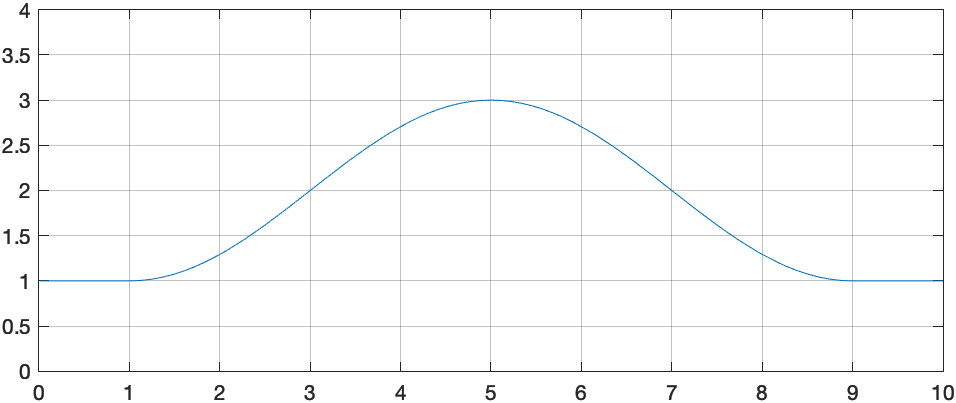
\includegraphics[width=\linewidth]{img/path.png}}
    \caption[Desired uDrone 2D path]{Desired uDrone path in defined state space}
    \label{fig:path}
\end{figure}

\subsection{Cost Function Parameters}

The cost function was determined directly from the motor parameters for the uDrone \parencite{t200}. Specifically, the force needed to pitch the vehicle was used to determine the angular velocity. The power necessary to create this force value is the control cost. Two methods were used for determining the cost, which are called "True" and "Zeroed" in this paper. The true method uses the exact motor values, including the constant force to move the vehicle forward. Therefore, this method takes into account drag. The zeroed approach normalizes the control cost to zero when there is no control input. This method will minimize control action, but not necessarily penalize the vehicle for following a path more closely if it also causes the vehicles to have a lower velocity in the X direction. The control cost curves can be seen in figure \ref{fig:cost}.

\begin{figure}[ht]
    \centerline{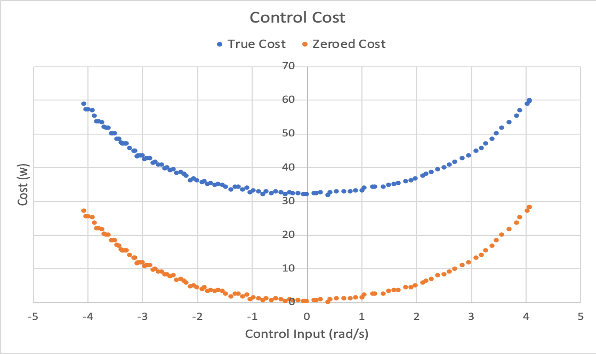
\includegraphics[width=\linewidth]{img/cost.png}}
    \caption[Control Cost]{Control cost for true (blue) and zeroed (orange) methods}
    \label{fig:cost}
\end{figure}

The ratio between control cost and tracking cost weight ($R$) was tested at three values, 0.01, 0.05, and 0.1. Since the values for control cost are in the double digit order of magnitudes and the value for tracking cost are in the single digit order of magnitudes, an $R$ value of 0.1 will treat the two costs as roughly equal. An $R$ value of 0.01 will make the tracking cost 10 times more important than control cost. 

\subsection{Discretization}
When discretizing, first a coarse trial was run at 10 Hz. After this was successful, more fine trials were run, up to 20 Hz. This timestep drove the step size for other variables via the constraint on moving forward in equation \ref{eq:dx}.
\begin{equation}
    \Delta x \leq v \cos \theta _{max} * \Delta t
    \label{eq:dx}
\end{equation}
Additionally, from the timestep the limits on control input are established, as seen in equation \ref{eq:control}.
\begin{equation}
\begin{split}
    \dot \theta = \Delta t * \ddot \theta\\
    -3.5 \leq \dot \theta\leq 3.5
\end{split}\label{eq:control}
\end{equation}
This, along with a desire to maintain fine discretization for grater accuracy, led to the final decision for discrete steps, as shown in table
\begin{center}
 \begin{tabular}{||c c c||} 
 \hline
 Value & Step Size & Step Count \\ [0.5ex] 
 \hline\hline
 x & 0.005 m & 2001 \\ 
 \hline
 y & 0.01 m & 401 \\
 \hline
 $\theta$ & $\frac{\pi}{24}$ rad & 23 \\
 \hline
 U & 0.05 $\frac{rad}{s}$ & 15\\
 \hline
\end{tabular}
\end{center}

\begin{figure}[t]
\centering
\subfigure{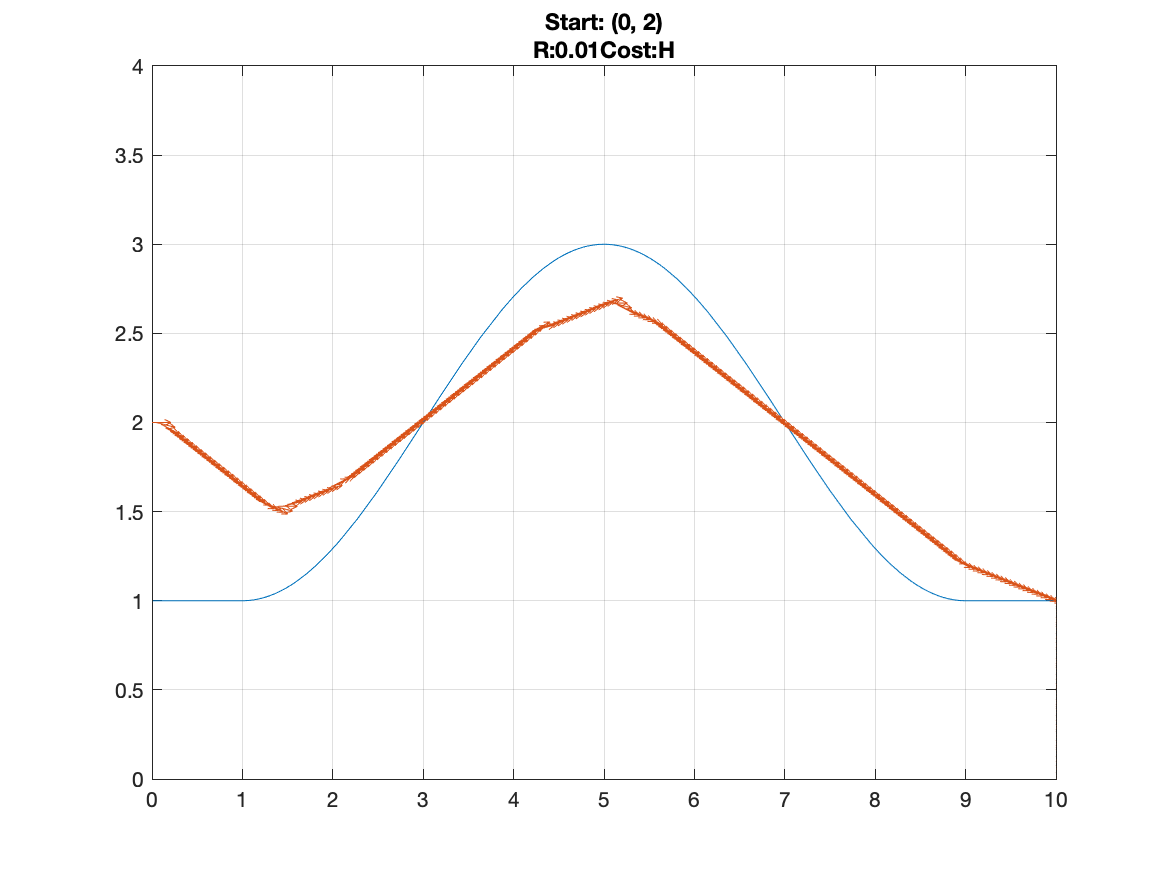
\includegraphics[width=0.32\linewidth]{img/R0_01_true.png}}
\subfigure{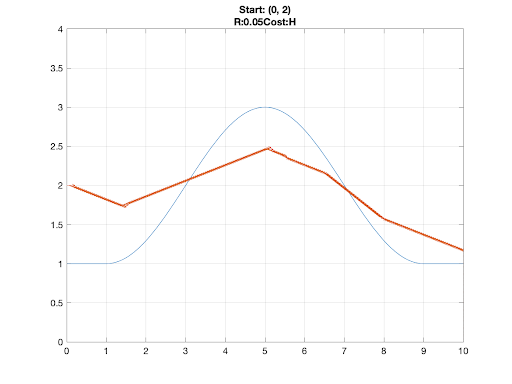
\includegraphics[width=0.32\linewidth]{img/R0_05_true.png}}
\subfigure{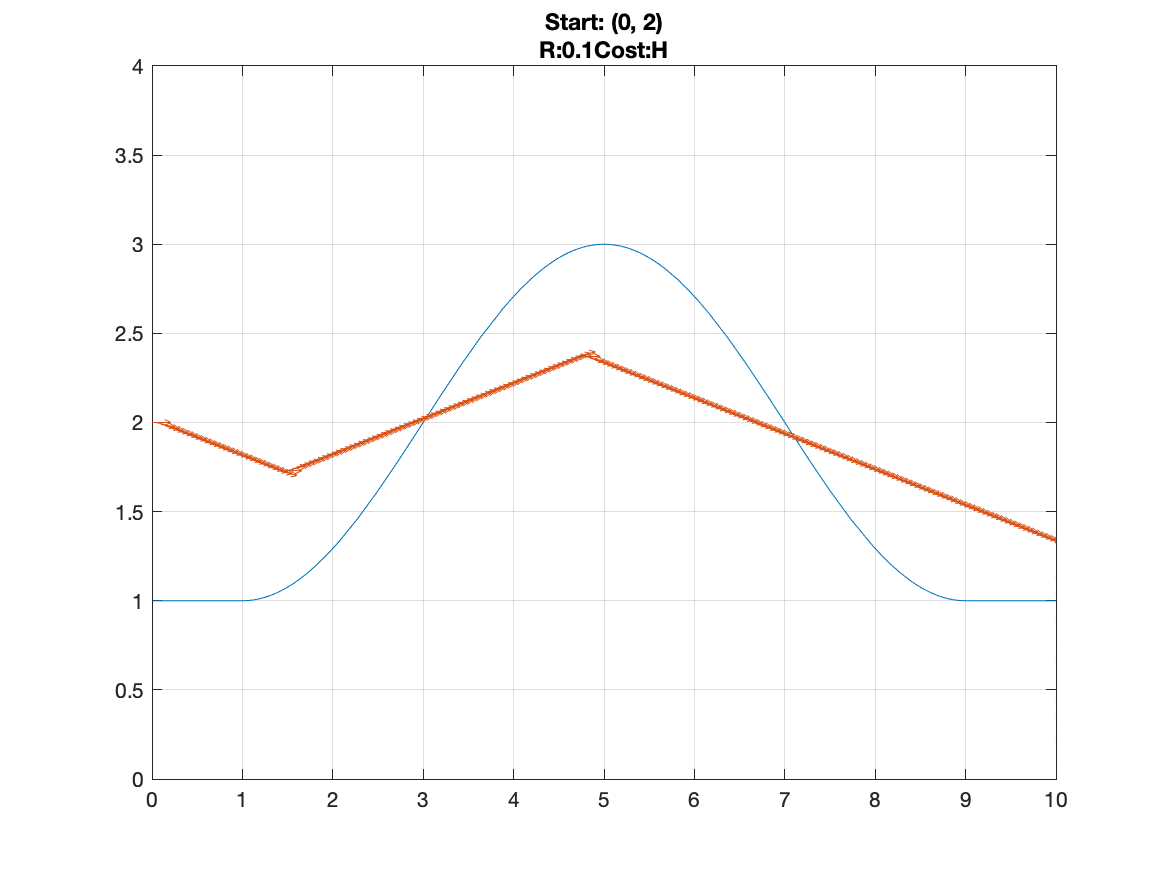
\includegraphics[width=0.32\linewidth]{img/R0_1_true.png}}
\caption[Optimal path using true cost]{Optimal path using true cost method for various R values (Left) R = 0.01 (Center) R = 0.05 (Right) R = 0.1}
\label{fig:true}
\end{figure}

\begin{figure}[t]
\centering
\subfigure{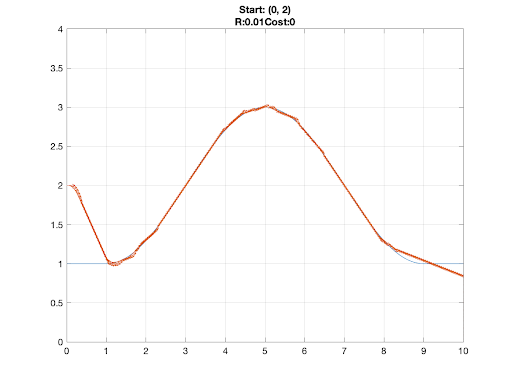
\includegraphics[width=0.32\linewidth]{img/R0_01_zero.png}}
\subfigure{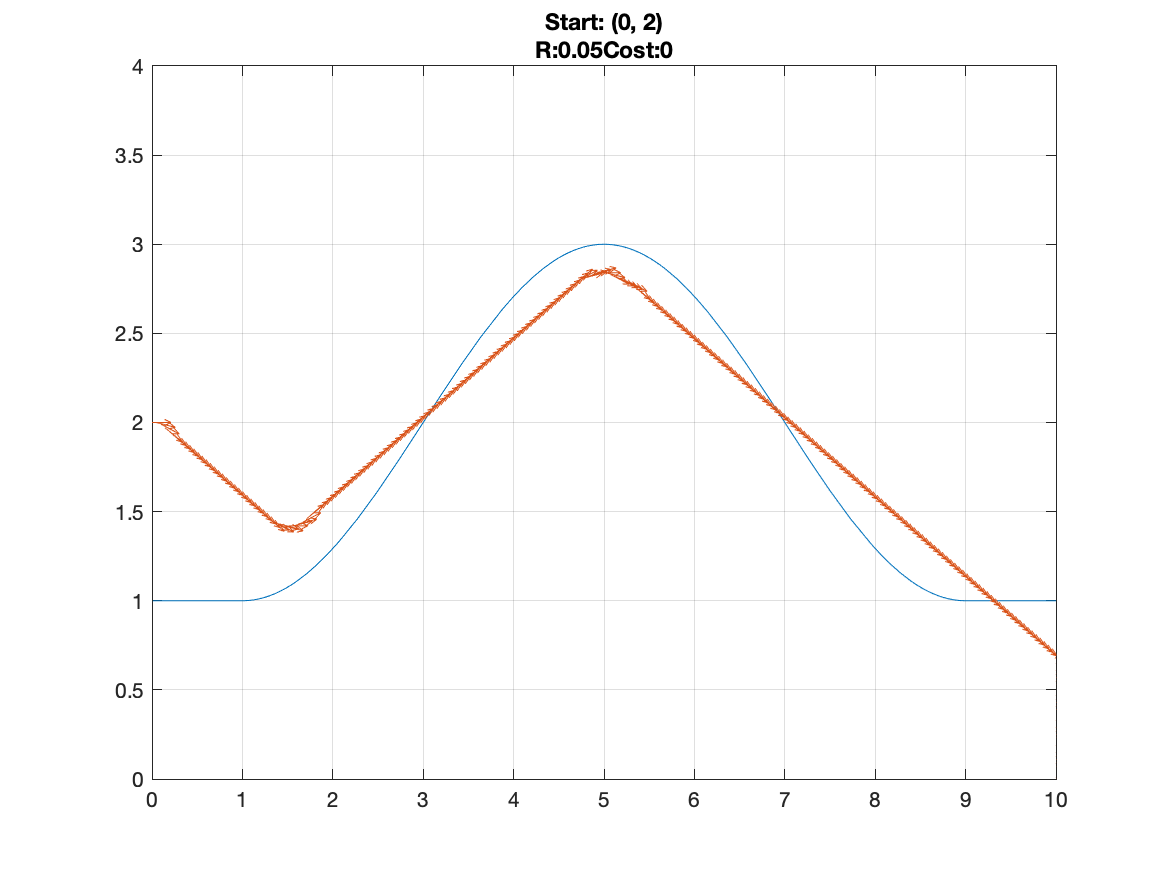
\includegraphics[width=0.32\linewidth]{img/R0_05_zero.png}}
\subfigure{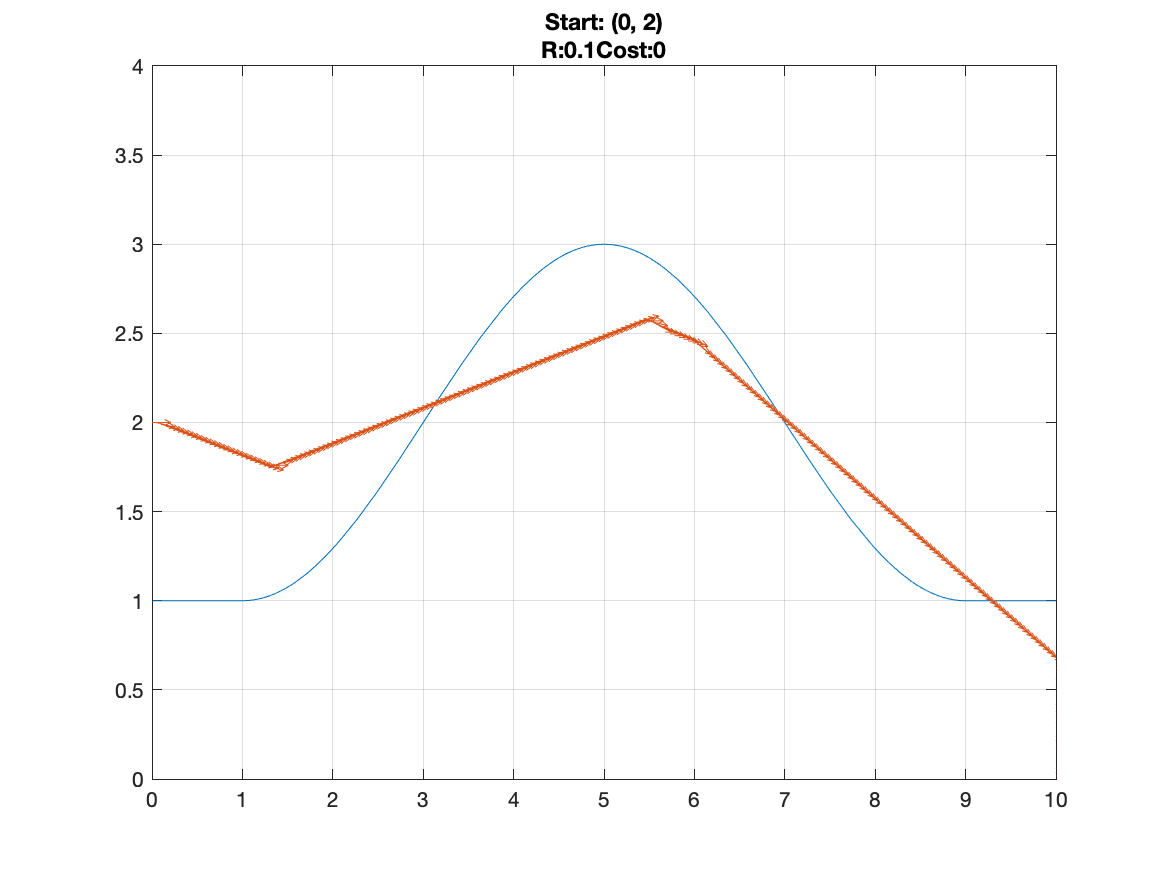
\includegraphics[width=0.32\linewidth]{img/R0_1_zero.png}}
\caption[Optimal path using zero cost]{Optimal path using zero cost method for various R values (Left) R = 0.01 (Center) R = 0.05 (Right) R = 0.1}
\label{fig:zero}
\end{figure}
\section{Results}
Six total trials were run, each with a different cost function method and $R$ value. In each trial 3D optimal cost and optimal control tables are generated. Based on the size of discretization, each table had over 18 million entries and the full trial took approximately 5 hours to complete. Using this data, two graphs are generated: the optimal path and the optimal control law. 
\subsection{Optimal Path}
The first graph demonstrates the optimal path of a vehicle at a given starting point. This is useful for visualizing the vehicle motion and how much it follows the path, as shown in figures \ref{fig:true} and \ref{fig:zero}. There are several conclusions that can be drawn from these figures: 1) As the $R$ value increases, the vehicle deviates from the path more. This can be seen by comparing the graphs in figures \ref{fig:true} and \ref{fig:zero}, where the $R$ value increases from left to right. This makes sense as a lower $R$ value increases the weight of the path following relative to the control cost. 2) The true cost method causes the vehicle to deviate from the path more than the zeroed method. The true cost method also maintains the vehicle at a more horizontal orientation, thus increasing the component velocity in the X direction. This is shown by comparing figure \ref{fig:true} to figure \ref{fig:zero}. The result of the cost method comparison is intuitive since the cost to move forward will cause the optimal path to take the vehicle through the simulation in the least number of steps.

\subsection{Control Law}
The second graph is a visualization of the control law computed by the run. A control law is a table containing the optimal control choice at each state. This table would be loaded on to a vehicle and used to determine control, as running any dynamic programming problem in real time would be to computationally intensive and slow. Since it is not practical to display the full three-dimensional graph in this format, a slice is presented here. Figure \ref{fig:Ustar} shows a single slice of the control law. Specifically, this figure shows the control law for a given $x$ and $y$ when $\theta$ is equal to zero. In this figure the red color represents areas of positive (counterclockwise) optimal control, the blue color areas of negative (clockwise) optimal control, and the white areas of zero optimal control. 

\begin{figure}[h]
    \centerline{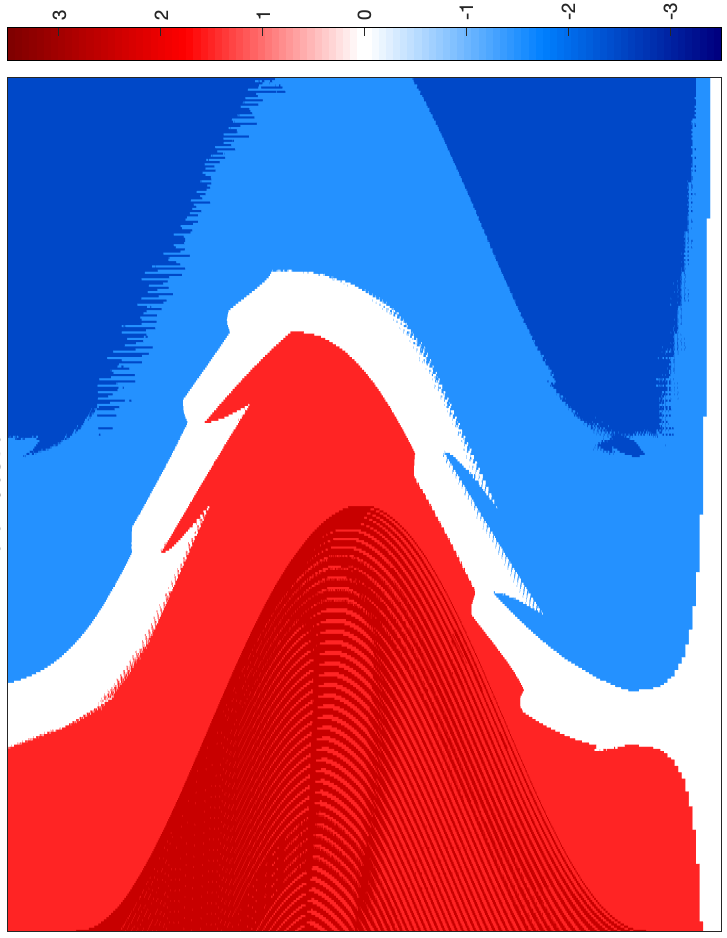
\includegraphics[width=0.5\linewidth]{img/U_star.png}}
    \caption{Optimal Control Law}
    \label{fig:Ustar}
\end{figure}

Clearly visible in the figure is the dark red lower parabola which is the very high cost area of hitting the reef that the control law tries to avoid. The lighter red areas are where the vehicle is behind or below the path and needs to pitch up to get on track. The light and dark blue areas are where the vehicle is above or in front of the path and needs to pitch down. The white band is when the vehicle is directly next to the path and should move straight in the body fixed axes.

% Two main methods of analysis were used - one with zeroed costs and one with the true cost. The true cost accounts for the cost associated with the constant movement of the drone. Since the the drone is always moving at a constant forward speed the true cost method penalized every movement step, so the optimal policy was in part searching for the shortest path. Zeroed cost was also helpful since the only considered input was the pitch rate, so it may be reasonable to ignore the cost of basic forward movements. Both were analyzed for varying values of R. There resulting optimal paths are shown in figure \ref{fig:zero} and in figure \ref{fig:true}. As can be seen, the analysis done with true cost cuts through the set path because there is a cost associated with travel distance. It is therefore optimal to make the trip in the shortest distance possible.




% In addition to plotting the optimal paths a plot showing the optimal control law is shown for each position $X$ and $Y$. where $theta$ is equal to $0$. The map is show in figure \ref{fig:Ustar}. The blue are represents a negative input while red represents a positive input. Note that this specific map is for the case with R = 0.01 and zeroed cost.






\section{Conclusions}
%The key conclusion is that a zeroed cost permits greater path following capacity. This is expected because there is no cost for a control input of 0. In other words, motion is not penalized as heavily in the zeroed cost case as in the true cost case. It is clear in the true cost case that the uDrone simply attempts to exit the grid as quickly as possible without hitting the reef even when $R$ is lowered. When considering the various $R$ values, the results are also as expected. The lower the R value, the greater the permissible control input which manifests itself in the results as greater path following. This is true in the zeroed and true cost cases, but is more evident in the latter case.

This project showed that dynamic programming is a valid method for creating an optimal control law for an underwater vehicle. Since this vehicle's mission is to travel in a straight plane, the simplifications from three to two dimensions would still allow for a usable control law. Additionally, the project showed the effects of the cost function on the optimal control policy. By varying the control cost calculation method (true versus zeroed) and changing the control weights (path following vs. control cost) the optimal trajectory changes. These trade offs need to be weighted based on the specific needs of the vehicle's mission. For example, if mapping fidelity and accuracy is paramount, a low $R$ value and zeroed cost would be best. But, if coverage is more important, a higher $R$ value and the true cost method are best. 

The largest barrier to practical implementation is the compute time and static environment needed for dynamic programming. The compute time issue can be overcome by pre-computing a control law, such as mentioned above. Dynamic programming is useful when the path is known in advance. This occurs when there are existing maps of survey regions or the vehicle is returning to a site it previously visited. However, given the variable topography of reefs, it would be hard to pre-compute a control policy for exploration. In these cases, other optimal methods could be used such as model predictive control or optimal path generation with PID control. 

% Some general conclusions which can be gleaned from these results are: the "nearest neighbor" apprproach sacrifices accuracy in favor of speed, discretization of the states and controls limit smooth action, simple models can yield great intuition, and that zeroing the cost permits greater path following capacity.

% Looking forward to future research, the team would explore this program running onboard the uDrone with a finite horizon. It would require precomputing the J* and U* tables. Other solution methods would also be explored, especially Model Predicitve Control (MPC) and Calculus of Variations.
% \begin{figure}[t]
%     \centerline{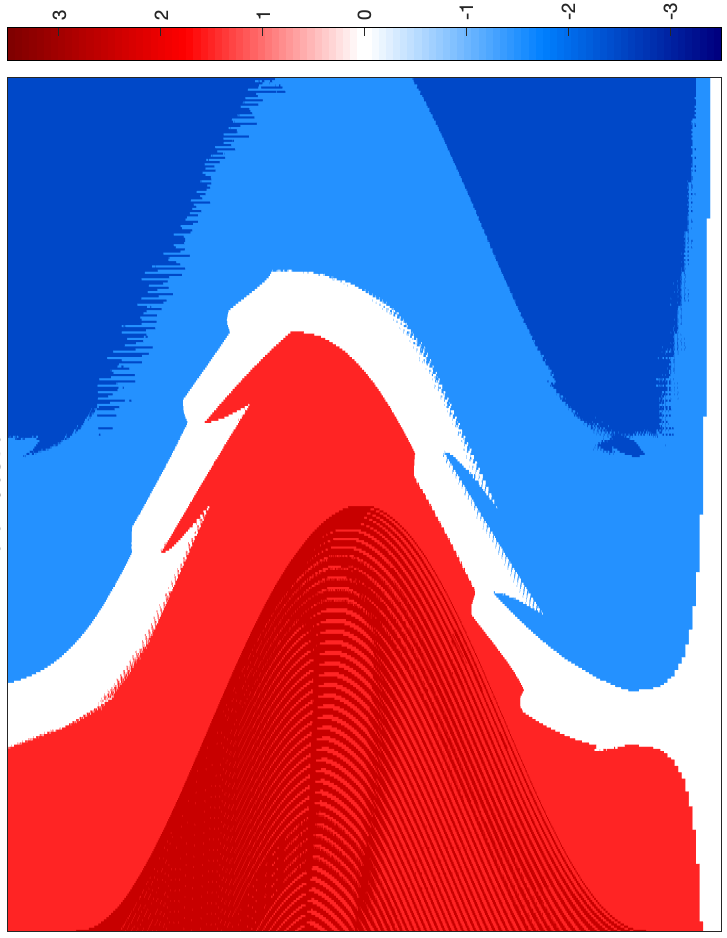
\includegraphics[width=\linewidth]{img/U_star.png}}
%     \caption{Optimal Control Law}
%     \label{fig:Ustar}
% \end{figure}

\chapter{PID Control in Simulation Environment}

The primary goal of this thesis project is to create a vehicle that satisfies the needs of the GDCS coral monitoring projects. Specifically, the uDrone needs to be able to follow the contour of the reef at a set distance. In order to show that this is possible, a simulation environment was developed that shows this capability. The details of how this simulation environment was created and the results are detailed in this section.\footnote{The software for this application was written jointly by the author and A.L.G. Prasad, another member of the DREAMS Lab who is working on uDrone autonomy. Help and code snippets were also provided by Harish Anand, another DREAMS Lab member.} 

\section{Methods}

This trial features a simulated uDrone following the terrain contours of a known reef profile. In order to do this, a simulation environment was built, a controller was developed and a contour profile was measured.  

\subsection{Simulation Environment Setup}

A world was created in Gazebo that contained a reef model. In this case, the reef model obtained by me using 3D motion capture while scuba diving was used. The model was scaled to a near realistic size. The world not only has the reef topography but also as a photographic overlay of the reef. UUV sim was also used in the simulated world. This allowed for mimicking some of the characteristics of water, such as buoyant forces and hydrodynamic damping. 

The uDrone model was added to the word file. This particular uDrone model was outfit with a downward-facing, broad-beam, sonar. The particular sonar used was the hector gazebo sonar plugin \parencite{sonar}. The specifications of the simulated sonar are set up to match the Blue Robotics Ping Echosounder used in the actual uDrone. This meant a beam-width of 30 degrees was used.

An emulated instance of the PX4 flight stack was used for the direct motor control of the uDrone. This was done using the PX4 Software in the Loop (SITL) for simulation where the PX4 software is run on a software emulated flight controller. The air-frame configuration of the HippoCampus \textmu AUV was used as it very closely mimics the motor configuration of the uDrone. The MAVROS plugin for ROS was used to communicate with the PX4 flight stack over MAVLink. 

\subsection{ROS Setup}
\begin{figure}[h]
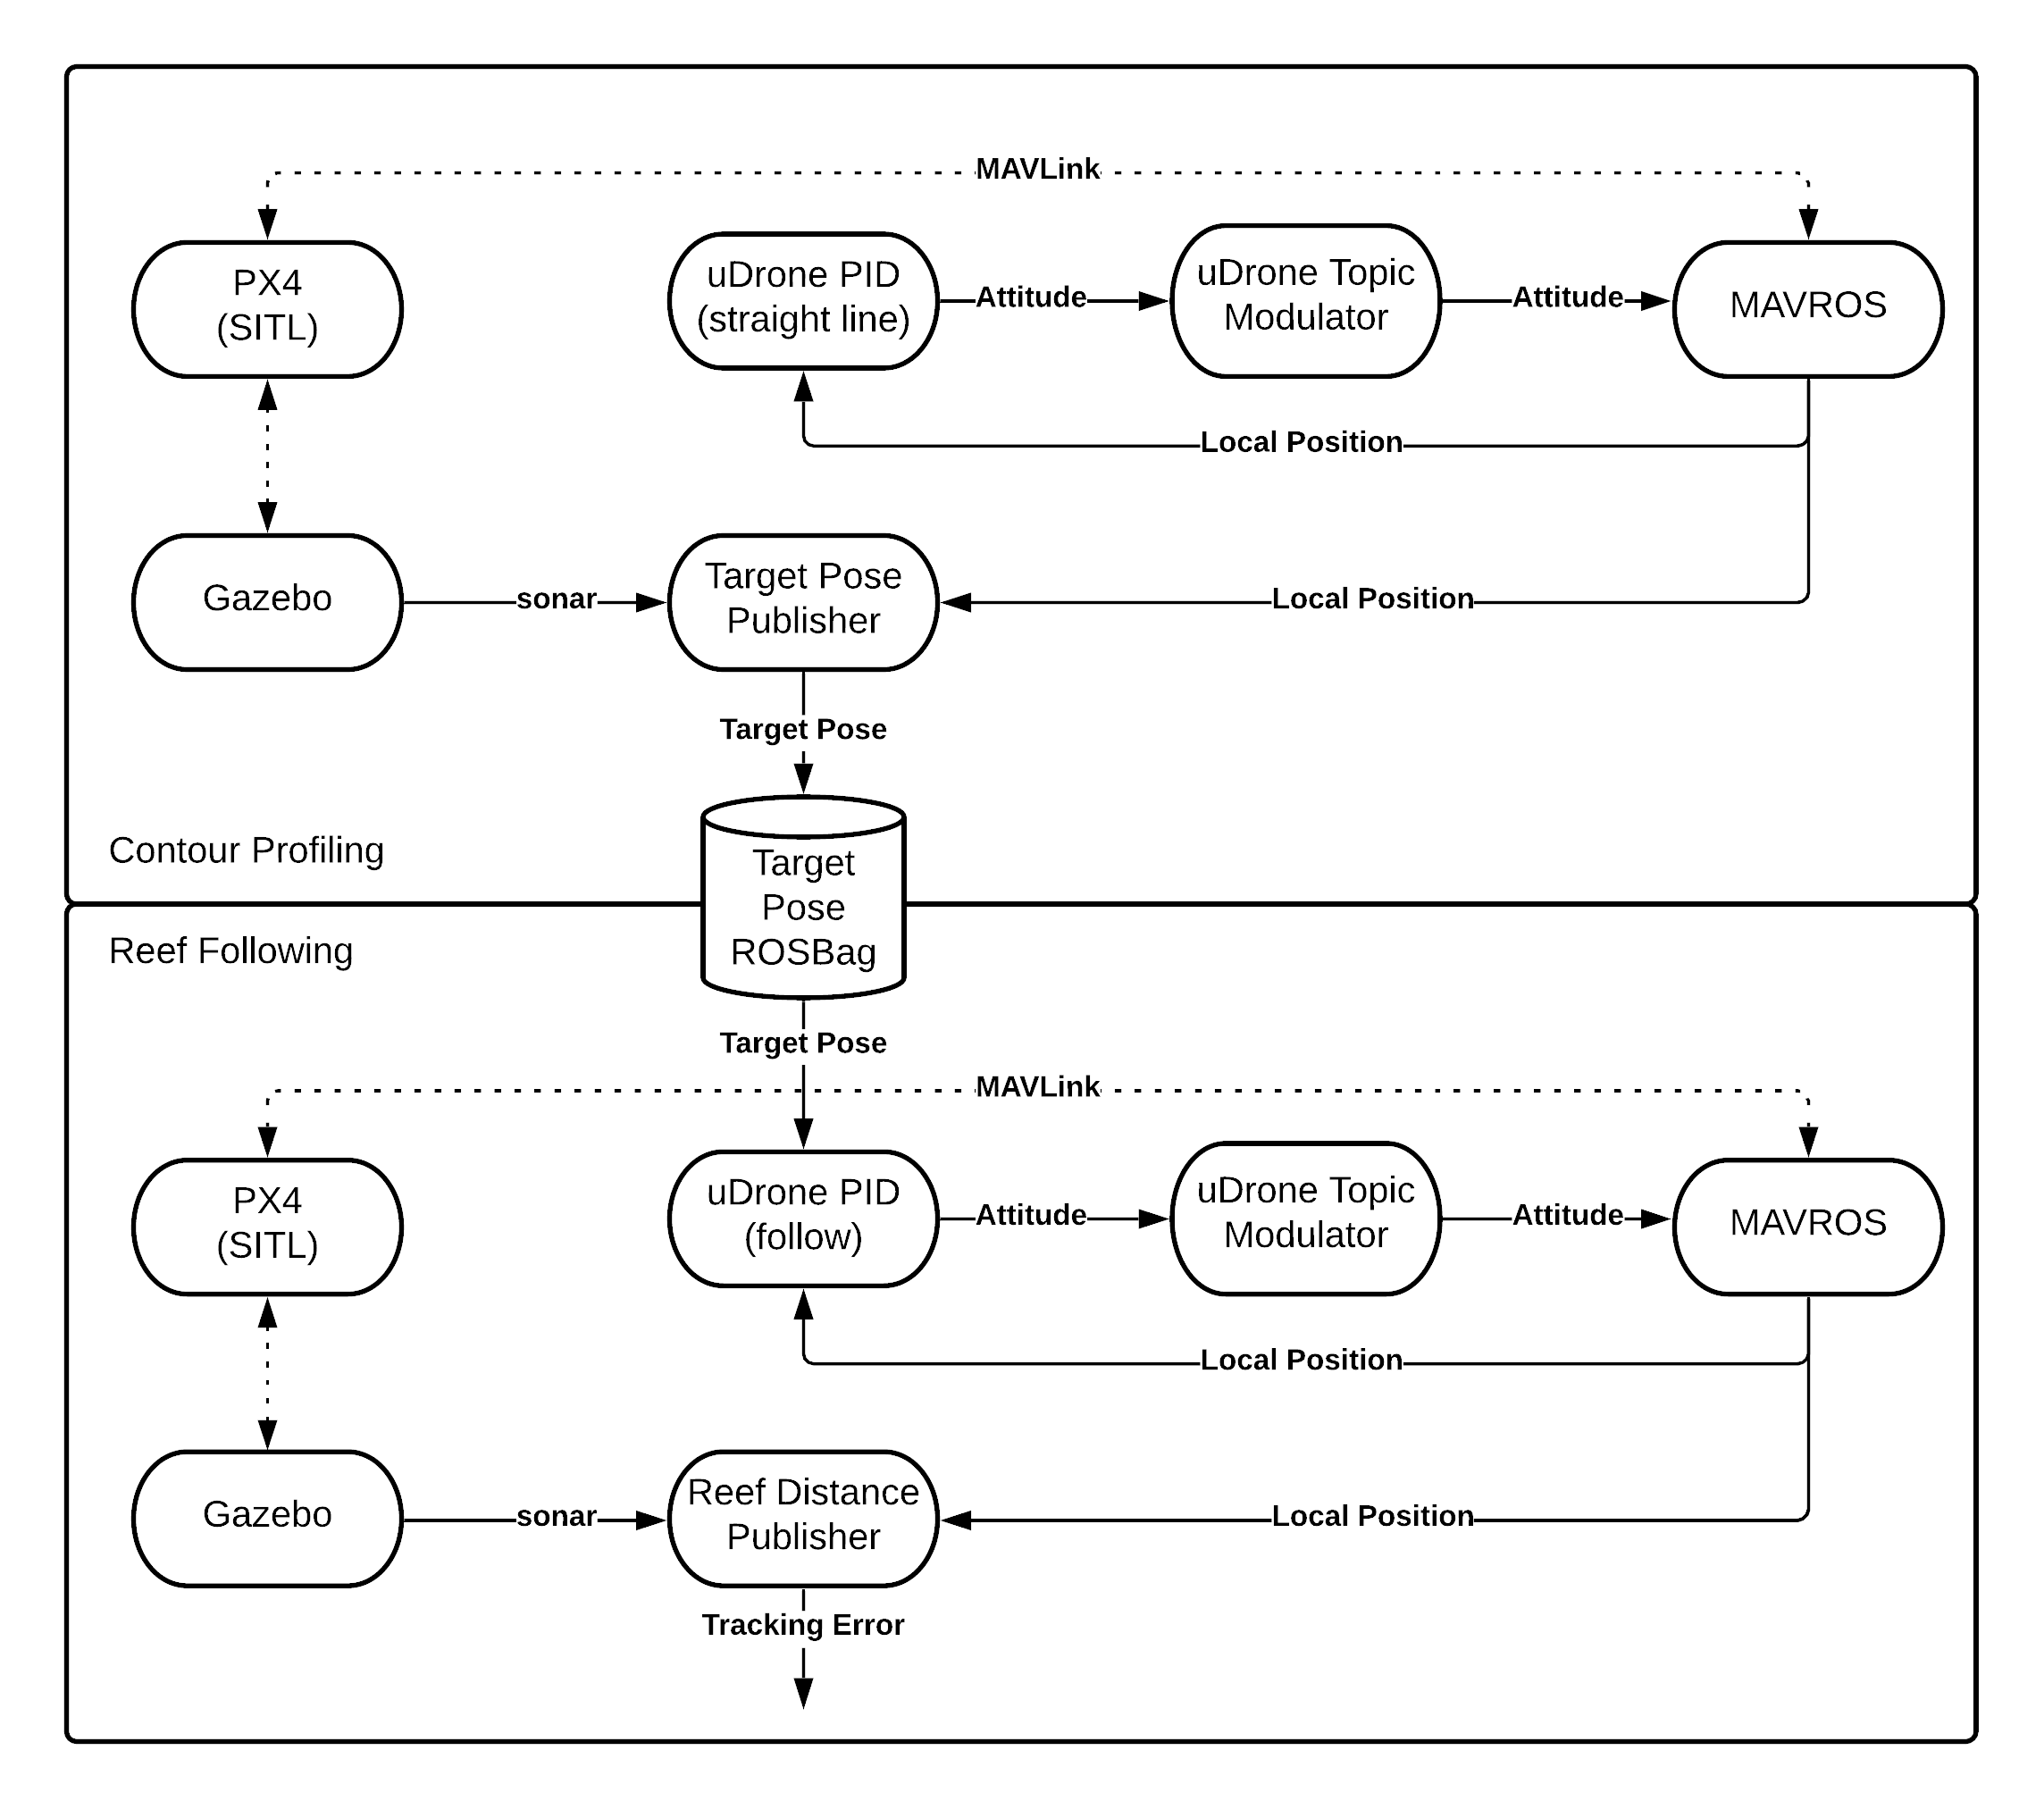
\includegraphics[width=\maxwidth{\textwidth}]{img/ros.png}
\caption{ROS Nodes for Contour Profiling and Reef Following in Simulation}
\label{ros}
\end{figure}

The program was broken into nodes following the ROS development model. The diagram of the node layout can be seen in figure \ref{ros}.

A special ROS node was created, called the uDrone Topic Modulator, in order to launch all of these components together and communication with the uDrone through MAVROS. This startup node’s launch file loaded the reef and uDrone into the Gazebo simulation and initiated PX4 SITL. A C++ program written as part of this node connected to the vehicle set the flight mode to “offboard,” and armed the vehicle. This process was necessary for the controller to begin sending messages over MAVLink to the uDrone for control. It also listened for commands from other nodes and sent them along to the uDrone via MAVROS. 

The PID controller was a separate node that took in the uDrone's local position via MAVROS along with a target position and pose. This node had two modes. In follow mode it listened for a target pose and then followed it. In contour profiling mode it followed a path set in the C++ code. The path used for this application was a straight line. The PID controller itself will be discussed in section \ref{controller}. 

A final node was developed that served two purposes, depending on the need. This is called the Target Pose Publisher or Reef Distance Publisher. This node took in the sonar data output from the simulated echosounder in Gazebo along with the local position from MAVROS. In the contour profiling cases it output the target pose, as described in section \ref{contour}.In the reef following case it output the tracking error, or distance to the reef, used to calculate the results in section \ref{pid-results}.

The element that connects the contour profiling with the reef following is a ROSBag. The ROSBag packages is a built in feature of ROS that allows for the recording of data while ROS is running. In this case it was used to record the target pose from the contour profiling run. Then it was played back during the reef following run in order to send the uDrone the desired pose and position. 

\subsection{Controller Development}\label{controller}

For this application, a proportional–integral–derivative (PID) controller was developed to control the movement of the uDrone. While the PID is developed as a single controller, it controls the position in all three directions independently. The proportional term was found by comparing the desired position to the local position, as reported by the internal position estimator in PX4. This local position is relative to the vehicles starting point and determined using an extended Kalman filter that fuses data from the PixHawks internal IMU, Gyroscope, and compass. The proportional gain is set to 0.5. The integral term is found by summing past proportional errors. In this case, only the past two errors are summed and the gain is set to 0.005. The derivative term is estimated by calculating the change in error from the last time-step to this time-step and dividing by the step size. The gain for the derivative term is 0.05. 

The PID controller outputs a vector with a direction and magnitude, essentially pointing towards where the vehicle should go and how fast it should go there. In order to convert this into a usable control the method from \cite{faf} is used.

\section{Contour profiling}\label{contour}

A trajectory for reef following needed to be developed in order to accomplish this task. To do this, the simulation environment was started in the same way as for the final trial. However, instead of following a reef relative path, the uDrone was given the desired path of a straight line across the reef. As the uDrone traversed the reef, it took samples of the distance to the reef using the sonar. The final reef following path would follow the same trajectory on the X-Y plane as this straight line uDrone run. At each of these X and Y points, a new depth (Z) was recorded for the desired location. This point was calculated by subtracting the sonar depth value from the local depth value and then adding one. In the end, a trajectory was calculated and recorded that followed the reef at a distance of one meter. 

\subsection{Reef Following}

Another instance of the simulation was initiated, with the uDrone starting in the same spot relative to the reef as in the previous, contour profiling, step. The PID controller node, in this case, listened for the trajectory on a ROS topic. As desired set-points were received the controller instructed the uDrone on how to move through MAVROS. Meanwhile, the sonar readings were recorded in order to analyze the reef following the performance. 

Figure \ref{follow_ss} shows the uDrone moving over the reef in simulation. The vehicle can be observed pitched up to follow the reef. The blue cone below it is a visual representation of the sonar sensor which outputs the distance to the reef. 

\begin{figure}[ht]
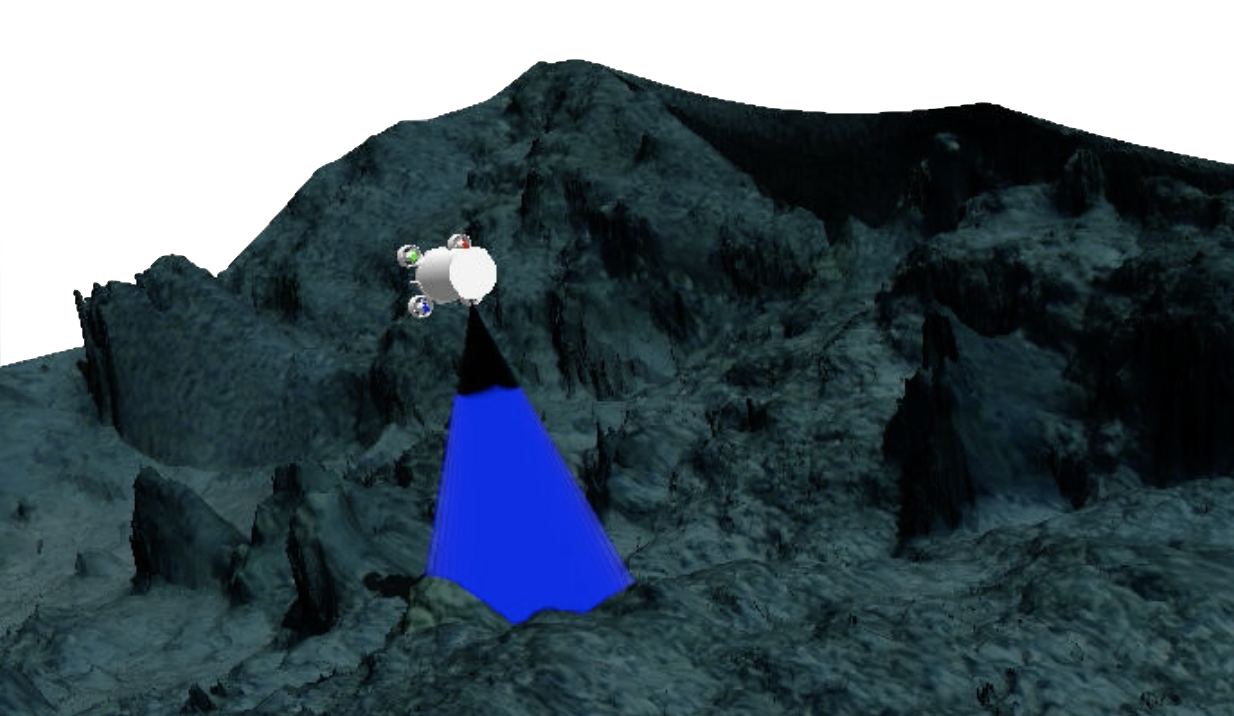
\includegraphics[width=\maxwidth{\textwidth}]{img/follow_ss.png}
\caption{uDrone During Reef Following in Simulation}
\label{follow_ss}
\end{figure}

\section{Results}\label{pid-results}

The uDrone was able to follow the profile of the reef as measured by the initial reef mapping. Figure \ref{follow} shows the results of this trial. The blue line is the path of the uDrone relative to it initial location. The gray line is the sonar reading which is the distance from the uDrone to the reef. Using these two together, the orange line is obtained, which is the position of the reef relative to the uDrone. The data starts at the 1m point, because it takes the uDrone some time and distance to reach a cruising altitude relative to the reef. 

\begin{figure}[h]
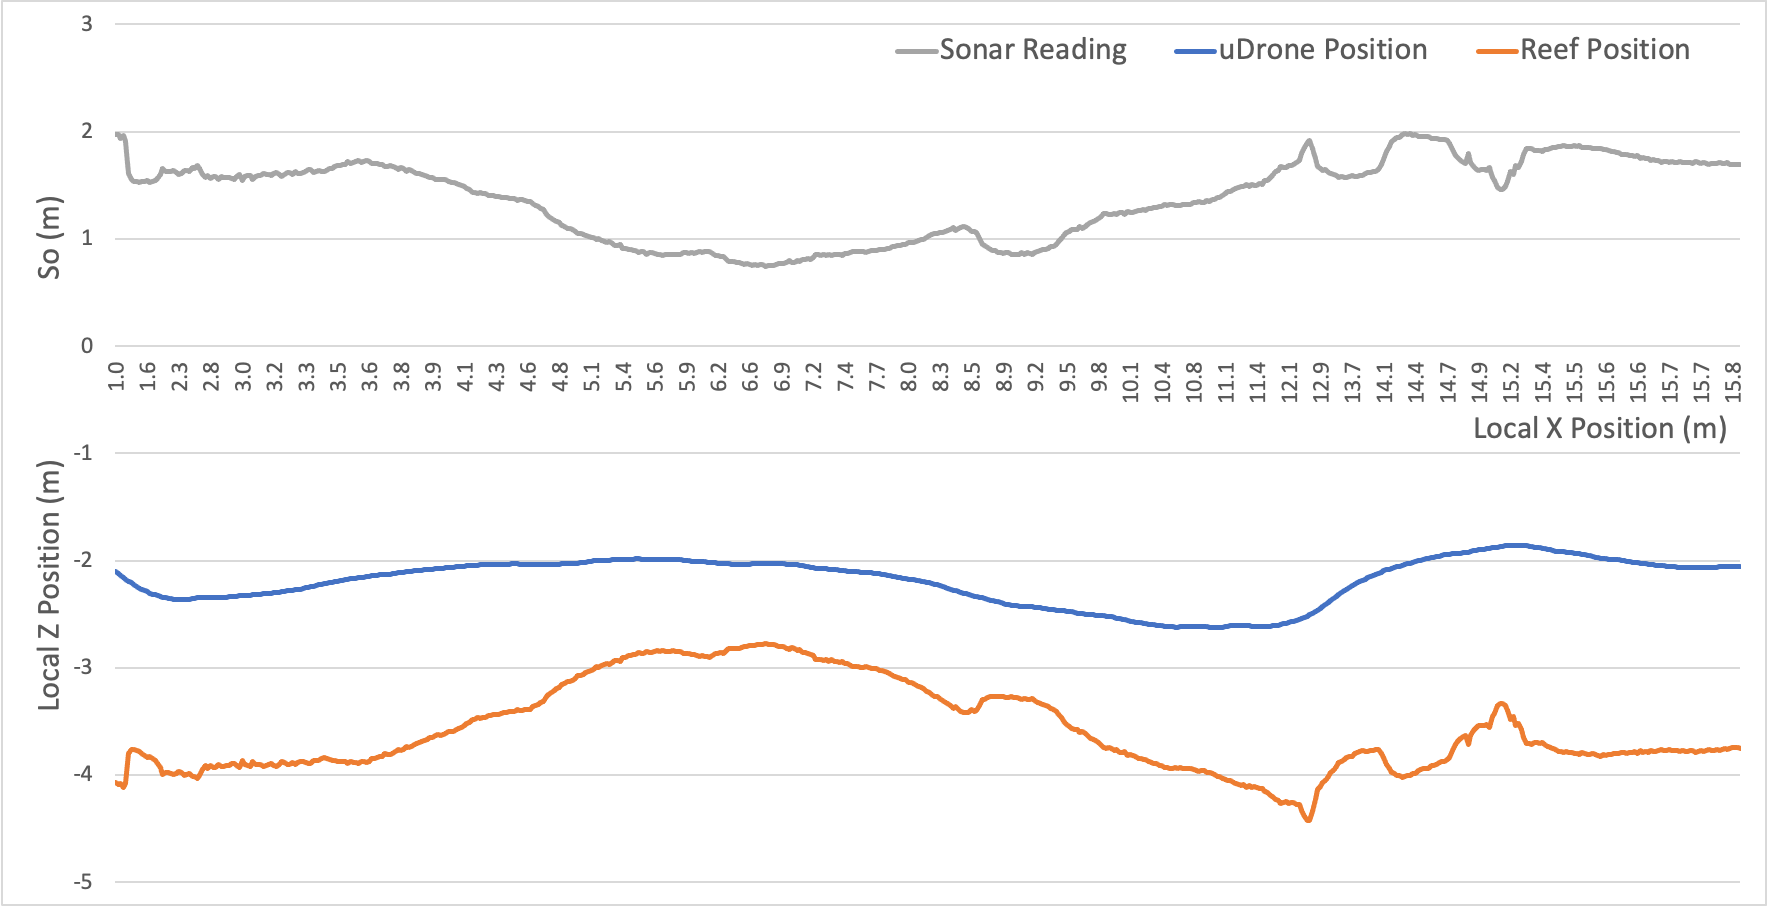
\includegraphics[width=\maxwidth{\textwidth}]{img/follow.png}
\caption{uDrone Reef Following Path and Sonar Reading}
\label{follow}
\end{figure}

As is shown in figure \ref{error}, the mean squared error is typically below 0.4. It gets as low as 0.15 as the vehicle spends more time at the desired height between the five and ten meter mark.  

\begin{figure}[h]
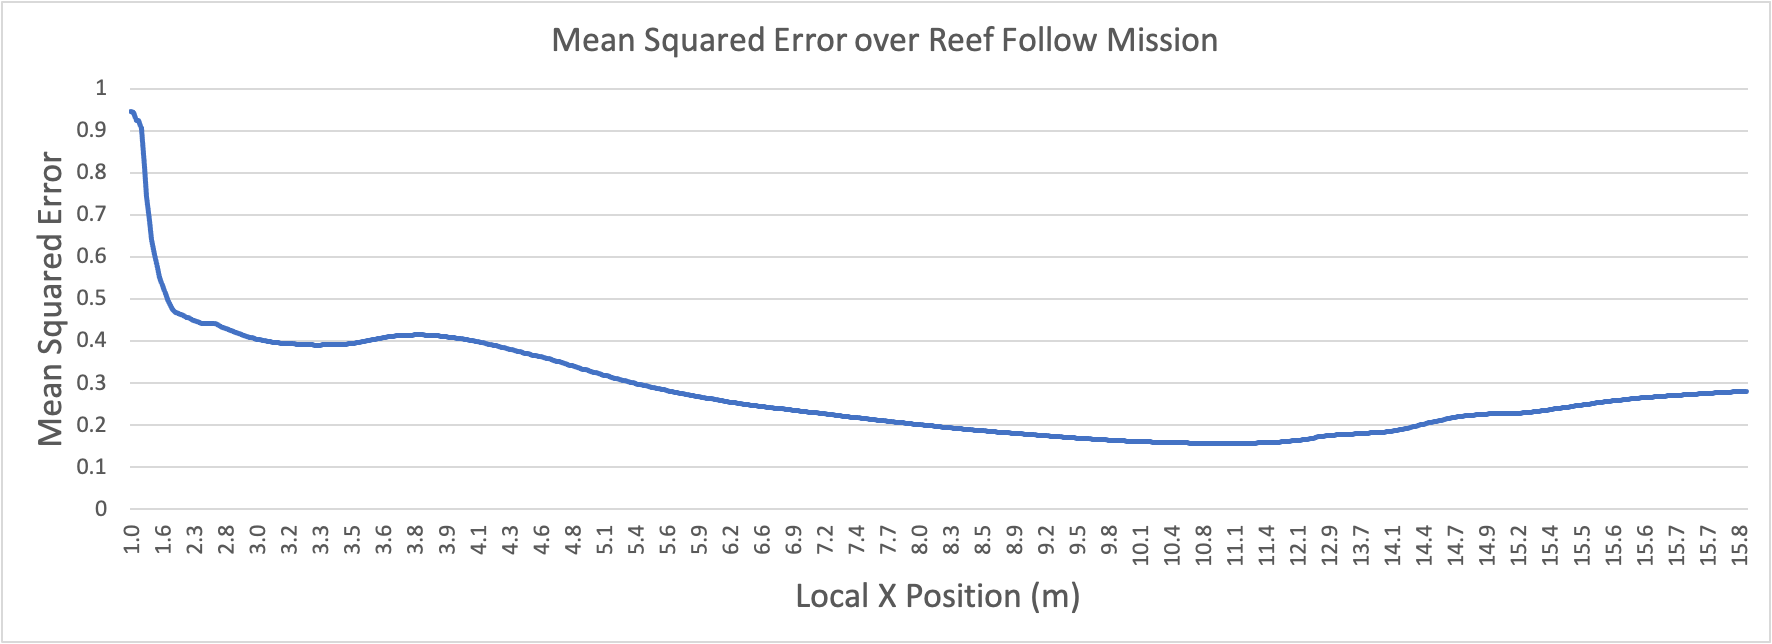
\includegraphics[width=\maxwidth{\textwidth}]{img/error.png}
\caption{Mean Squared Error over Reef Follow Mission}
\label{error}
\end{figure}
One major source of error in this method is the sonar. The sonar projects a cone and then averages the distance over that cone projection. This means the initial pass, which was roughly one meters above the reef, took a scan of a larger section of the reef than the follow pass. This means the desired location was based on the average distance to the reef of a bigger segment of the reef than that recorded when only one meter above the reef.

Another source of error is the PID controller itself. The tuning of this controller will effect how closely the vehicle stays to its desired path. While the uDrone PID was tuned so that it would generally work, it might not be the optimal tuning parameters.  

\section{Conclusion}

This experiment demonstrated that it is possible for the uDrone to practice reef following maneuvers with a PID controller and a known reef segment. As reef morphology data is collected for sections of reef, this method becomes more and more practical. Better resolution data for depth at various points will allow for even better results.

There are, however, drawbacks that would limit this approaches usefulness in a real world setting. First, localizing underwater is a difficult problem due to the lack of GPS. Therefore, it will be hard to start the uDrone from a known location relative to the reef from one trial to the next. This could be mitigated by using buoy to set start points, but that may requires adding man-made equipment to the reef. Second, this method relies on dead reckoning with the internal IMU to determine location. The error in the IMUs selected for the uDrone to not allow for dead reckoning over long distances, so some other method for localization must be used. And third, the reef is comprised of living organisms which may between trial times. The ideal situation is for the vehicle to use vision in real time to determine its path.
%\chapter{This is a chapter-level heading}

\lipsum[1]

\section{This is the first section-level heading}

% Test single- and double-spacing around block quotes
Nam dui ligula, fringilla a, euismod sodales, sollicitudin vel, wisi. Morbi auctor
lorem non justo. Nam lacus libero, pretium at, lobortis vitae, ultricies et, tellus. Donec
aliquet, tortor sed accumsan bibendum, erat ligula aliquet magna, vitae ornare odio
metus a mi. Morbi ac orci et nisl hendrerit mollis. Suspendisse ut massa. Cras nec ante.
Pellentesque a nulla. Cum sociis natoque penatibus et magnis dis parturient montes,
nascetur ridiculus mus. Aliquam tincidunt urna. Nulla ullamcorper vestibulum turpis.
Pellentesque cursus luctus mauris.
\begin{quote}
Nulla malesuada porttitor diam. Donec felis erat, congue non, volutpat
at, tincidunt tristique, libero. Vivamus viverra fermentum felis. Donec
nonummy pellentesque ante. Phasellus adipiscing semper elit. Proin
fermentum massa ac quam. Sed diam turpis, molestie vitae, placerat
a, molestie nec, leo. Maecenas lacinia. Nam ipsum ligula, eleifend at,
accumsan nec, suscipit a, ipsum. Morbi blandit ligula feugiat magna.
Nunc eleifend consequat lorem. Sed lacinia nulla vitae enim. Pellentesque
tincidunt purus vel magna. Integer non enim. Praesent euismod nunc eu
purus. Donec bibendum quam in tellus. Nullam cursus pulvinar lectus.
Donec et mi. Nam vulputate metus eu enim. Vestibulum pellentesque
felis eu massa.
\end{quote}
Quisque ullamcorper placerat ipsum. Cras nibh. Morbi vel justo vitae lacus tincidunt
ultrices. Lorem ipsum dolor sit amet, consectetuer adipiscing elit. In hac habitasse
platea dictumst. Integer tempus convallis augue. Etiam facilisis. Nunc elementum
fermentum wisi. Aenean placerat. Ut imperdiet, enim sed gravida sollicitudin, felis
odio placerat quam, ac pulvinar elit purus eget enim. Nunc vitae tortor. Proin tempus
nibh sit amet nisl. Vivamus quis tortor vitae risus porta vehicula.

\subsection{This is the first sub-section-level heading}

% Make sure single- and double-spacing around blocks works with line breaks in the source
Nam dui ligula, fringilla a, euismod sodales, sollicitudin vel, wisi. Morbi auctor
lorem non justo. Nam lacus libero, pretium at, lobortis vitae, ultricies et, tellus. Donec
aliquet, tortor sed accumsan bibendum, erat ligula aliquet magna, vitae ornare odio
metus a mi. Morbi ac orci et nisl hendrerit mollis. Suspendisse ut massa. Cras nec ante.
Pellentesque a nulla. Cum sociis natoque penatibus et magnis dis parturient montes,
nascetur ridiculus mus. Aliquam tincidunt urna. Nulla ullamcorper vestibulum turpis.
Pellentesque cursus luctus mauris.

\begin{quote}
Nulla malesuada porttitor diam. Donec felis erat, congue non, volutpat
at, tincidunt tristique, libero. Vivamus viverra fermentum felis. Donec
nonummy pellentesque ante. Phasellus adipiscing semper elit. Proin
fermentum massa ac quam. Sed diam turpis, molestie vitae, placerat
a, molestie nec, leo. Maecenas lacinia. Nam ipsum ligula, eleifend at,
accumsan nec, suscipit a, ipsum. Morbi blandit ligula feugiat magna.
Nunc eleifend consequat lorem. Sed lacinia nulla vitae enim. Pellentesque
tincidunt purus vel magna. Integer non enim. Praesent euismod nunc eu
purus. Donec bibendum quam in tellus. Nullam cursus pulvinar lectus.
Donec et mi. Nam vulputate metus eu enim. Vestibulum pellentesque
felis eu massa.
\end{quote}

Quisque ullamcorper placerat ipsum. Cras nibh. Morbi vel justo vitae lacus tincidunt
ultrices. Lorem ipsum dolor sit amet, consectetuer adipiscing elit. In hac habitasse
platea dictumst. Integer tempus convallis augue. Etiam facilisis. Nunc elementum
fermentum wisi. Aenean placerat. Ut imperdiet, enim sed gravida sollicitudin, felis
odio placerat quam, ac pulvinar elit purus eget enim. Nunc vitae tortor. Proin tempus
nibh sit amet nisl. Vivamus quis tortor vitae risus porta vehicula.

\subsubsection{This is the first sub-sub-section-level heading}

\lipsum[1]

\paragraph{This is the first paragraph-level heading}

\lipsum[1]

\subparagraph{This is the first sub-paragraph-level heading}

\lipsum[1]

\section{Citation examples}

The contents of this section differ depending on the bibliography settings, specifically whether the `usebiblatex' toggle is set to `true' or `false'.
\iftoggle{usebiblatex}{%
  This sentence shows citation with biblatex \parencite{searchinger_world_2013}.
  This is another sentence showing citation with biblatex \parencite{pathak_rural_2007}.
}{%
  This sentence shows citation with natbib \citep{pathak_rural_2007}.
  This is another sentence showing citation with natbib \citep{searchinger_world_2013}.
}

\section{Footnote examples}

This is a sentence followed by a footnote.\footnote{Mauris ut leo. Cras viverra metus rhoncus sem. Nulla et lectus vestibulum urna fringilla ultrices. Phasellus eu tellus sit amet tortor gravida placerat. Integer sapien est, iaculis in, pretium quis, viverra ac, nunc. Praesent eget sem vel leo ultrices biben- dum. Aenean faucibus. Morbi dolor nulla, malesuada eu, pulvinar at, mollis ac, nulla.}
This is another sentence followed by a footnote.\footnote{Mauris ut leo. Cras viverra metus rhoncus sem. Nulla et lectus vestibulum urna fringilla ultrices. Phasellus eu tellus sit amet tortor gravida placerat. Integer sapien est, iaculis in, pretium quis, viverra ac, nunc. Praesent eget sem vel leo ultrices biben- dum. Aenean faucibus. Morbi dolor nulla, malesuada eu, pulvinar at, mollis ac, nulla.}

\section{Block quote example}

The following is a block quote:

\begin{quote}
\lipsum[1-2]
\end{quote}

\section{Endnote examples}

Endnotes appear in a separate section after chapters and before the reference list.
This is a sentence followed by a endnote.\pagenote{Mauris ut leo. Cras viverra metus rhoncus sem. Nulla et lectus vestibulum urna fringilla ultrices. Phasellus eu tellus sit amet tortor gravida placerat. Integer sapien est, iaculis in, pretium quis, viverra ac, nunc. Praesent eget sem vel leo ultrices biben- dum. Aenean faucibus. Morbi dolor nulla, malesuada eu, pulvinar at, mollis ac, nulla.}
This is another sentence followed by a endnote.\pagenote{Mauris ut leo. Cras viverra metus rhoncus sem. Nulla et lectus vestibulum urna fringilla ultrices. Phasellus eu tellus sit amet tortor gravida placerat. Integer sapien est, iaculis in, pretium quis, viverra ac, nunc. Praesent eget sem vel leo ultrices biben- dum. Aenean faucibus. Morbi dolor nulla, malesuada eu, pulvinar at, mollis ac, nulla.}
And here is a really long endnote to show formatting across several pages.\pagenote{\expandafter\lipsum[1-6]}

\section{Table example}

See table \ref{table\arabic{tablecounter}} for an example of a table.
Place macros inside captions using \string\macrocapwrap.
See table \ref{table\arabic{tablecounter}} for a demonstration.

\begin{table}[h] % Table float
\caption{Here is a table caption that is especially long to show what happens when it extends to more than one line in the table of contents}
\label{table\arabic{tablecounter}}
\begin{tabu}{l c c} \\ \hline
Column1 & Column2 & Column3 \\ \hline
Row1 & 2.0 & 3.0 \\
Row2 & 2.0 & 3.0 \\
Row3 & 7.0 & 8.0 \\ \hline
\end{tabu}
\legend{\emph{Source}: Here is a source note that is especially long to show what happens when it extends to more than one line.}
\legend{\emph{Note}: Here is a note that is especially long to show what happens when it extends to more than one line.}
\end{table}
\refstepcounter{tablecounter}

\begin{table}[h] % Table float
\caption{This table caption refers to another caption: see figure \macrocapwrap{\ref{figure1}} }
\label{table\arabic{tablecounter}}
\begin{tabu}{l c c} \\ \hline
Column1 & Column2 & Column3 \\ \hline
Row1 & 2.0 & 3.0 \\
Row2 & 2.0 & 3.0 \\
Row3 & 7.0 & 8.0 \\ \hline
\end{tabu}
\end{table}
\refstepcounter{tablecounter}

\section{Figure example}

See figure \ref{figure\arabic{figurecounter}} for an example of a figure.

\begin{figure}
\includegraphics[width=\maxwidth{\textwidth}]{antidorcas.jpg}
\caption{Antidorcas marsupialis, male}
\label{figure\arabic{figurecounter}}
\legend{\emph{Source}: \iftoggle{usebiblatex}{\textcite{krishnappa_adult_2012}}{\citet{krishnappa_adult_2012}}}% See: https://upload.wikimedia.org/wikipedia/commons/8/89/Antidorcas_marsupialis%2C_male_%28Etosha%2C_2012%29.jpg
\legend{\emph{Note}: Here is a note that is especially long to show what happens when it extends to more than one line.}
\end{figure}
\refstepcounter{figurecounter}
\clearpage
\section{Math examples}

This section contains some math-heavy text adapted from \iftoggle{usebiblatex}{\textcite{dwilkins1995}}{\citet{dwilkins1995}}.
In non-relativistic wave mechanics, the wave function $\psi(\mathbf{r},t)$ of a particle satisfies the Schrödinger Wave Equation
%
\begin{equation}
 i\hbar\frac{\partial \psi}{\partial t}
  = \frac{-\hbar^2}{2m} \left(
    \frac{\partial^2}{\partial x^2}
    + \frac{\partial^2}{\partial y^2}
    + \frac{\partial^2}{\partial z^2}
  \right) \psi + V \psi.
\end{equation}
%
It is customary to normalize the wave equation by
demanding that
%
\begin{equation}
\int \!\!\! \int \!\!\! \int_{\textbf{R}^3}
      \left| \psi(\mathbf{r},0) \right|^2\,dx\,dy\,dz = 1.
\end{equation}
%
A simple calculation using the Schr\"{o}dinger wave
equation shows that
%
\begin{equation}
\frac{d}{dt} \int \!\!\! \int \!\!\! \int_{\textbf{R}^3}
      \left| \psi(\mathbf{r},t) \right|^2\,dx\,dy\,dz = 0,
\end{equation}
%
and hence
%
\begin{equation}
\int \!\!\! \int \!\!\! \int_{\textbf{R}^3}
      \left| \psi(\mathbf{r},t) \right|^2\,dx\,dy\,dz = 1
\end{equation}
%
for all times~$t$. If we normalize the wave function in this
way then, for any (measurable) subset~$V$ of $\textbf{R}^3$
and time~$t$,
%
\begin{equation}
\int \!\!\! \int \!\!\! \int_V
      \left| \psi(\mathbf{r},t) \right|^2\,dx\,dy\,dz
\end{equation}
%
represents the probability that the particle is to be found
within the region~$V$ at time~$t$.

\begin{table}[h] % Table float
\caption{This caption has math characters that remain lowercase: \relax\macrocapwrap{$\psi(\mathbf{r},t)$} }
\label{table\arabic{tablecounter}}
\begin{tabu}{l c c} \\ \hline
Column1 & Column2 & Column3 \\ \hline
Row1 & 2.0 & 3.0 \\
Row2 & 2.0 & 3.0 \\
Row3 & 7.0 & 8.0 \\ \hline
\end{tabu}
\end{table}
\refstepcounter{tablecounter}

\chapter{Conclusion}

A novel underwater, open source, and configurable vehicle that can support experiments with both scientific and engineering goals was designed, constructed, and tested in simulation. Propulsion and sensor tests were carried out in a pool, in preparation for autonomy field tests. This final chapter will review the contributions of this thesis and discuss the ongoing and future work. 
% \section{Controller Comparison}
% -practical for use in real life, which control method is better
\section{Contribution}
% What new knowledge was created?
A need for the uDrone was demonstrated. It will allow for greater volumes of coral reef imaging data to be obtained in a safe and reliable manner. Additionally, the uDrone will continue to produce advances in underwater autonomous navigation research from its joint simulation and real world testbed.

This thesis detailed the chosen hardware and software components and explained how they fit together. This system configuration could be used to develop underwater vehicles with similar technical capabilities. 

The mathematical model of the vehicle dynamics will allow for future controller development. Specifically, this work can be used to create a model predictive controller which could greatly improve controllability of the uDrone. 

The two control methods discussed in this document demonstrate how the uDrone navigates through a reef environment. In particular, the code written for the PID controller can be used for future research and development of autonomous controllers.

\section{Ongoing Work}

Work on the uDrone has continued as this thesis drew to a conclusion. This section discusses two areas where work is currently ongoing. 

\subsection{Water Testing}
An initial set of tests has been conducted in a pool. This can be seen in Figure \ref{pool-test} and the video can be viewed at the URL associated with \cite{jd-pool}. The first goal of these tests was to validate the waterproofing of the vehicles. The enclosure and seals are able to seal out water and the electronics were kept dry. The second goal is to test ballasting and buoyancy. The vehicle was very slightly positively buoyant, which is desirable. The center of gravity was slightly below the center of buoyancy, but in the same line. This caused the uDrone to sit horizontally in the water and have a slight moment to keep itself upright in roll, which is ideal. Finally, the vehicle dynamics were tested. This involved manually piloting it around the pool and verifying that it was agile and controllable. While there is no concrete measurement for this, it qualitative performed very well in the water.

\begin{figure}[ht]
    \centering
    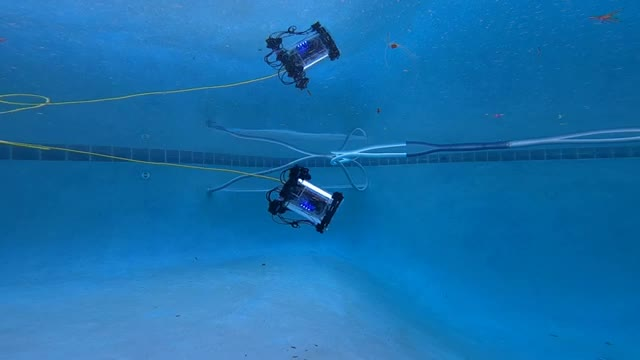
\includegraphics[width=\maxwidth{\textwidth}]{img/pool-test.jpeg}
    \caption{uDrone in the pool during a propulsion test}
    \legend{\emph{Source}: \cite{jd-pool}}
    \label{pool-test}
\end{figure}

\subsection{Diver-Following}

The testbed has allowed for proof of concept tests of vision based navigation. The first of these tests is being run by a DREAMS Lab member and uDrone contributor, A.L.G. Prasad. Using the same PID controller developed as part of this thesis, he was able to write code to enable the uDrone to follow a scuba diver in simulation. This is only the first step in the Vision Based Navigation track, but it is a meaningful step towards autonomy. 

\section{Future Work}\label{future-work}

Despite the achievements laid out here, there is still substantial work that need to be performed for the uDrone to operate in a fully autonomous mode. The two most pressing areas of immediate future work are water tests and vision based navigation.

\subsection{Vision Based Navigation}

The end goal of the uDrone project is for it to be able to navigate unknown environments using vision. This will include aspects of visual-inertial odometry (VIO) and simultaneous localization and mapping (SLAM). Both of these fields are well developed on land but are still emerging in the underwater realm. For example, \cite{mono-vio} developed a method for visual odometer in turbid water using an inexpensive camera. Or, as previously mentioned, \cite{manderson2020visionbased} shows a working application of underwater visual based navigation. Tools and datasets, like AQUALOC, are being created which can aid in the training of vision-based machine-learning algorithms for navigation \parencite{aqualoc}. Underwater visual based navigation is a prime area of research right now and with the uDrone, DREAMS Lab and ASU are well positioned to become contributors and leaders in this area. 

\subsection{Real-World Water Testing}
The next set of pool tests will verify that the uDrone can be autonomously controlled via ROS. Then, once it has been thoroughly tested in a controlled and confined environment, the uDrone will be taken to Hawaii where it will be tested in a real coral environment. The first few tests will include divers following the vehicle to watch for any issues. Eventually, it can complete its first solo autonomous missions.

\subsection{Reinforcement Learning}

With enough trails and data from the real world and an improved simulation it will be possible to create a controller for the uDrone based on reinforcement learning. This has the potential to be both more efficient and more robust than a PID or MPC. This new controller would be trained in simulation using collected data from real world experiments. It may employ other, pre-trained, vision algorithms or be trained as a full end-to-end algorithm. 

\subsection{Hardware Configuration}

Several improvements can already be suggested for the uDrone hardware based on insights yielded from this thesis. Primarily, it was determined that switching the flat front plate of the enclosure to a domed plate would reduce the hydrodynamic drag on the uDrone and allow for the camera to be positioned at different angles. Additionally, more cameras can be added to the body at different angles in order to improve the vision based navigation that will come in the next phase.

In order to continue improving the vehicle configuration, several hardware experiments can be run. The first and most straightforward of these experiments is to test the impact of adjusting the vehicle's ballast. This would allow for different behaviors of the vehicle, which may be desirable for different types of missions. Furthermore, alternative thruster configurations can be tested. For example, if all the thrusters are pitched outward, then the uDrone would have some minimal control authority to move in the Y or Z directions independently of rotating. This would have the drawbacks of being less efficient for motion in the X direction and greatly complicating any models or model based controllers that have been developed. 

%\subsection{Alternative Configurations}
% - Domed front: More hydrodynamics, variable angles of camera
% - Multicamera: Up, Down
% - Thruster Configuration: Tilt out: allow for movement in different directions, move to CB/CG, more hydrobatics


                                        % Heading commands (in descending order):
                                        % \chapter
                                        % \section
                                        % \subsection
                                        % \subsubsection
                                        % \paragraph
                                        % \subparagraph
%%%%%%%%%%%%%%%%%%%%%%%%%%%%%%%%%%%%%%%
% Back matter
%%%%%%%%%%%%%%%%%%%%%%%%%%%%%%%%%%%%%%%
\SingleSpacing                          % Back matter should be single spaced
\AfterEndEnvironment{table}{\SingleSpacing} % Reset these environments
\AfterEndEnvironment{figure}{\SingleSpacing}
\AfterEndEnvironment{quote}{\SingleSpacing}
\AfterEndEnvironment{quotation}{\SingleSpacing}


\edef\defaulttolerance{\the\tolerance}
\tolerance 500                          % Increase tolerance to prevent material extending into margins
\hbadness 500

\iftoggle{useendnotes}{%                % If you're using endnotes, output them here
  \setsecnumdepth{none}                 % No section numbering in end notes
  \bookmarksetup{startatroot}           % Make Notes appear at root level of PDF bookmarks
  \phantomsection%                      % Need for hyperref
  \addcontentsline{toc}{chapter}{%      % Add a chapter-level heading for
    \hspace{-\cftchapterindent}%        %  Notes to the ToC
    \notesname%
  }%
  \renewcommand*{\notedivision}{%
    \chapter*{\notesname}%
  }
  \printpagenotes                       % Output the notes
  \setsecnumdepth{all}%                 % Turn section numbering back on after printing
}{}

\bookmarksetup{startatroot}
\chapter*{\bibheading}                  % In the running text, use a chapter-level heading
                                        % for the bibliography section
\phantomsection
\addcontentsline{toc}{chapter}{%        % In the TOC, add a custom chapter-level heading
  \hspace{-\cftchapterindent}%          % that will be flush against the left margin
  \bibheading%
}
%\phantomsection
%\addtocontents{toc}%                    % Add this 'mark' to TOC so subsequent pages use
%  {\protect\markboth{\bibheading}{Page}}%   the bibliography heading (unlikely since
%                                        %   the appendices follow quickly)
\iftoggle{usebiblatex}{%                % Output the bibliography
  \printbibliography[heading=none]      % Using a 'biblatex' package; do not let
                                        %   'biblatex' output a heading
}{%
  \renewcommand\bibsection{}            % Do not let 'natbib' output a heading
  \bibliographystyle{\natbibstyle}      % Using 'natbib' to print bibliography
  \bibliography{\bibfilename}
}

% \appendix                               % Indicate start of appendices
%                                         % Appendices are considered 'mainmatter' in this
%                                         %   documentclass
% \tolerance \defaulttolerance            % Set tolerance back to default
% \hbadness \defaulttolerance

% \addtocontents{toc}{\protect%           % Only include appendix title in table of contents
%   \setcounter{tocdepth}{0}}%            %   and omit sub-headings
% \renewcommand*{\chapnamefont}%          % Reset font for 'Appendix' in chapter titles
%     {\normalfont\MakeTextUppercase}
% \makeatletter                           % Clear page after printing appendix title
%   \renewcommand{\memendofchapterhook}%
%   {%
%     \clearpage
%     \m@mindentafterchapter
%     \@afterheading
%   }
% \makeatother

% \phantomsection                         % Need '\phantomsection' to place hyperref
%                                         %   bookmark more accurately
% \addcontentsline{toc}{part}{Appendix}   %~Add "Appendix" to TOC here; comment out this
%                                         %   line if you're not including appendices

%\phantomsection                        %!This is the one part of the template that I
%\addtocontents{toc}%                   %   could not get to work properly. After you
%  {\protect\markboth{APPENDIX}{Page}}  %   start listing appendices in the TOC,
                                        %   subsequent TOC pages should use "APPENDIX in
                                        %   the header instead of "CHAPTER"; however,
                                        %   this code will make "APPENDIX" appear on the
                                        %   the same page that the *first* appendix
                                        %   appears on. This problem won't affect most
                                        %   people, but if it affects you, uncomment
                                        %   these lines and move them below where
                                        %   the appendices are listed. Keep moving these
                                        %   lines down and checking the output until
                                        %   the TOC headers appear correctly

%\include{appendix1}                     %~Insert your appendices here; I recommend to use
%\include{appendix2}                     %   \include rather than \input for appendices.
%\include{appendix3}% etc.               %   All heading commands are the same as above,
                                         %   e.g., \chapter, \section, etc.

\backmatter                             % Start back matter according to documentclass
\makeatletter                           % Do not clear page after printing title for
\renewcommand{\memendofchapterhook}%  %   biographical sketch
  {%
    \m@mindentafterchapter
    \@afterheading
    \hspace{-\cftchapterindent}
  }
\makeatother

\biographicalsketch{%                  %~Biographical Sketch is optional
 % \chapter*{Biographical Sketch}

Alex Goldman is a Master's of Science student in the Robotics and Autonomous Systems program with a concentration in Artificial Intelligence at Arizona State University and a member of the Distributed Robotic Exploration and Mapping Systems Laboratory. Before attending ASU for his Master's, Alex started several entrepreneurial ventures and worked as a project lead on large projects involving both hardware and software. This led Alex to be an ideal candidate to take on the uDrone project, which leveraged his leadership experience while furthering his engineering education. Alex has had a lifelong interest in the aquatic environment and reef conservation. He started scuba diving at the age of 11 and at 19 he became a certified Scuba instructor. During his undergrad at the University of Michigan, he was one of the leaders of the Human Powered Submarine Team. After school, he volunteered as a scuba diver at the Shedd Aquarium in Chicago. He even proposed to his wife underwater. This is all to say: Alex has been personally interested in scuba diving and reef conservation for a very long time.%                   %<Enter the name of the .tex file containing your
}%                                     %   biography or omit this line and type in
                                        %   your biography here (1 paragraph)
\end{document}
